\chapter{Results} \label{chapter:resutls}

\section{Exploring model architecture}
\subsection{Introduction}
\paragraph{}
During this study we explored different way to build an efficient architecture for our task. This process required a lot of trial and measurement. The goal of this section is to illustrate and explain the different choice made during the choice of the final architecture. In this optic we will cover different topic, starting with the choice of the input size, followed by the position of the detection layers, and we will then explore the details of the feature extraction part of the network.

\subsection{Input size} \label{sec:inputSize}
\paragraph{}
During this study we explored different input resolution to run our model. This point is the most critical point in our study, as we mainly focus on speed. It is expected that the number of computation needed by a fully convolutional architecture such as the one we use here is linearly correlated to the input size. This linearity can be observed on Figure \ref{fig:latencysize}. But at the same time, the lower the resolution of the image, the less information are available to allow detection. This is particularly true for small sign that may become invisible. However, our study use case allow such sign not to be very accurately detected as they will get bigger as the car move closer to them.

We choose to keep the original image aspect ratio recorded by smartphone camera to maintain the semantic as the one human are used to, reducing also the deformation created by small rotation of the objects and keeping the symmetry of the information loss on both axis. From that we explored different size to see if they are good enough for a human to use. Figure \ref{resizeExample} show clear example of this. As you can see, the scaling induce a lot of information loss, but the information remaining is still enough for a human being to spot the sign on the image, leading to believe that a convolutionnal neural network can perform the same operation.

\begin{figure}
  \begin{center}
    \begin{subfigure}[t]{.49\linewidth}
      \centering
      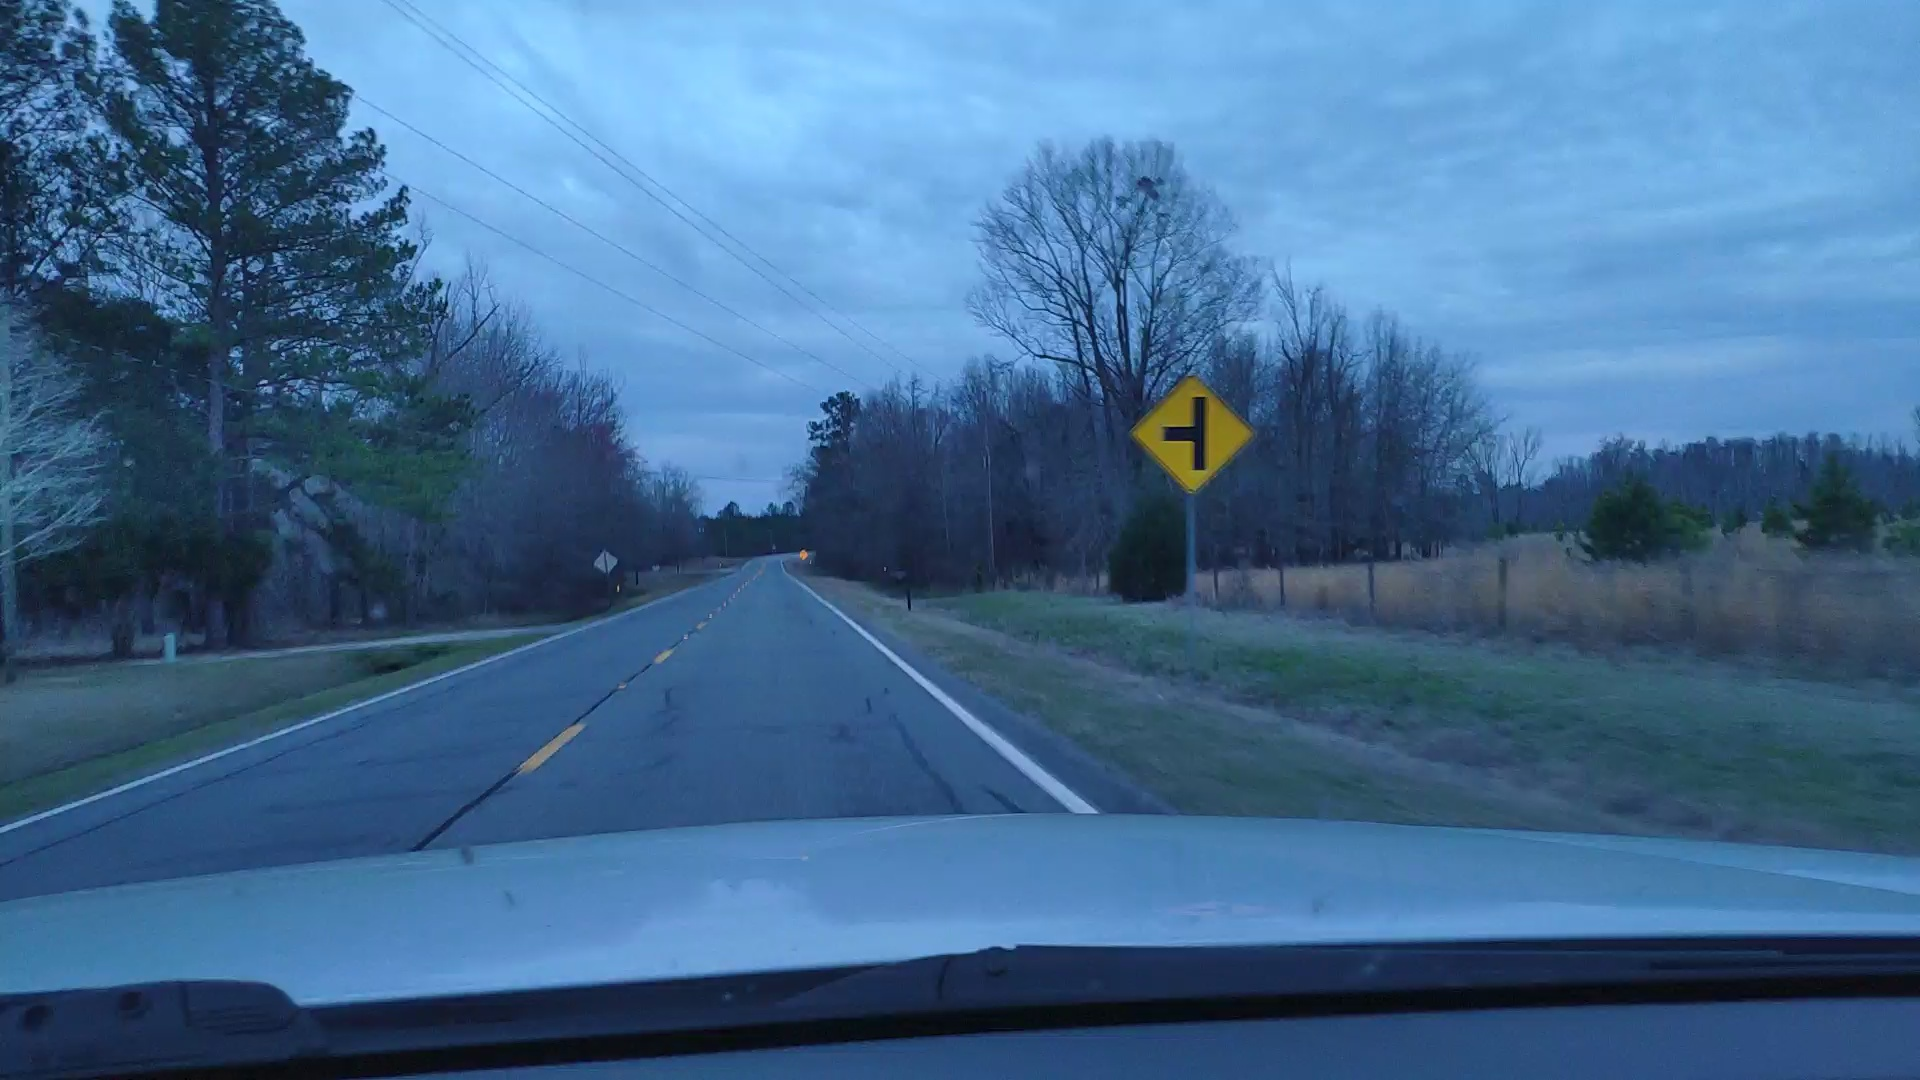
\includegraphics[width=0.99\linewidth]{figures/im_example_full.jpg}
      \caption{Full resolution image, $1080\times1920$}
    \end{subfigure}
    \begin{subfigure}[t]{.49\linewidth}
      \centering
      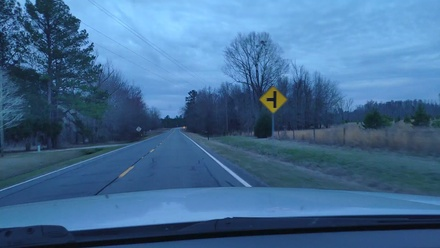
\includegraphics[width=0.99\linewidth]{figures/im_example_440x800.jpg}
      \caption{Image resized at $440\times800$}
    \end{subfigure}
    \begin{subfigure}[t]{.49\linewidth}
      \centering
      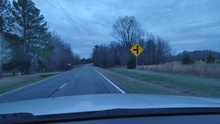
\includegraphics[width=0.99\linewidth]{figures/im_example_220x400.jpg}
      \caption{Image resized at $220\times400$}
    \end{subfigure}
    \begin{subfigure}[t]{.49\linewidth}
      \centering
      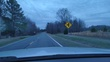
\includegraphics[width=0.99\linewidth]{figures/im_example_110x200.jpg}
      \caption{Image resized at $110\times200$}
    \end{subfigure}
    \caption{Example of an image resized at different size and displayed at same size. This image contains two signs, one on the foreground, clearly visible, and another one at the level of the forest in the background. This second one is clearly visible on a full screen image at full resolution, but quickly disappear as resolution drop, while the bigger one stay clear.}
    \label{resizeExample}
  \end{center}
\end{figure}

\begin{figure}
  \begin{center}
    \begin{subfigure}[t]{.49\linewidth}
      \centering
      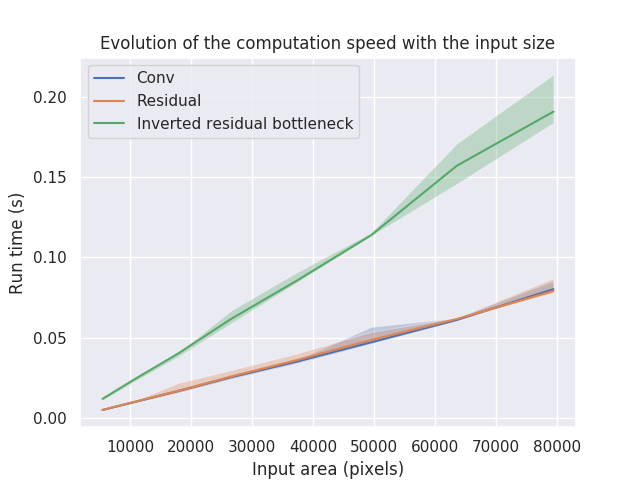
\includegraphics[width=0.99\linewidth]{figures/speed_by_nn_size_and.png}
      \caption{Latency evolution with input size}
      \label{fig:latencysize}
    \end{subfigure}
    \begin{subfigure}[t]{.49\linewidth}
      \centering
      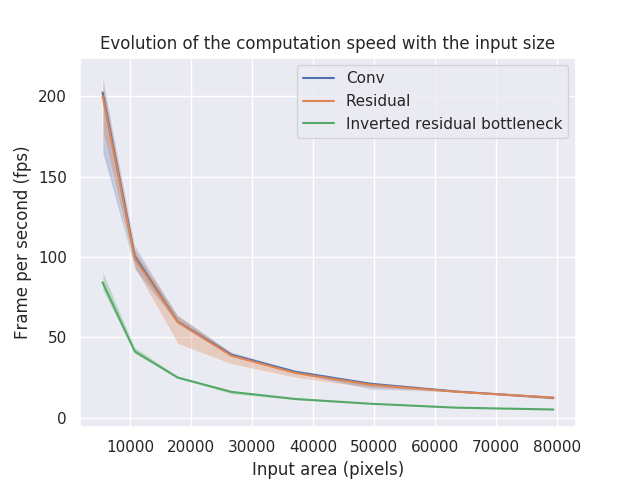
\includegraphics[width=0.99\linewidth]{figures/speed_by_nn_size_fps_and.png}
      \caption{FPS evolution with input size}
      \label{fig:fpssize}
    \end{subfigure}
    \caption{Evolution of the prediction speed for different block type. The input area represent the number of pixel in the input image. These results were obtained by running a TensorFlow Lite version of the model on Samsung S6 (SM-920T) on one thread. The hard line represent the average value, while the area go from the minimum to the maximum value over all runs.}
    \label{resizeExample}
  \end{center}
\end{figure}

% add experiment about the size / accuracy ?
We first experimented with image at $220\times400$ resolution, however, as the accuracy was good we decided to step down to $110\times200$. This smaller resolution also gave us a good accuracy while reducing the number of computation by a factor $4$.

\subsection{Detection layers position} \label{sec:detectionLayerPos}
\paragraph{}
The layers doing the detection of the signs are located at two different position of the network. This to allow more local features to be taken into account for small object while larger object have a larger activation area.

A statistical analysis of our dataset performed following the same idea as in \cite{yolov3}. We chose to use five different anchors. These anchors are given in Table \ref{tab:anchors}. This set of anchors give us an average IoU over our dataset of $75.28\%$, showing the drawback of the assumption chosen previously, but also showing that they are valid if you do not want perfect boxes. This anchors boxes are completely compatible with the activation area there corresponding layers as displayed on Table \ref{tab:activationArea}.

Because of the assumption we chose in Chapter \ref{chapter:technicalApproach}, Section \ref{Assumptions}, the number of bounding boxes our model can predict is limited and have given position. These boxes depend on multiple factor, the anchor size, but also the general architecture of the backbone network as well as the input size. Figure \ref{fig:anchors} represent all the different box our model can predict, displaying clearly the limit of our assumptions in term of accuracy, but giving enough coverage of the space to provide good results.

\begin{figure}
  \begin{center}
    \begin{subfigure}[t]{.49\linewidth}
      \centering
      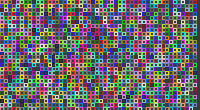
\includegraphics[width=0.99\linewidth]{figures/anchors/boxes_layers_0.png}
      \caption{Every possible boxes for anchor $3\times3$}
    \end{subfigure}
    \begin{subfigure}[t]{.49\linewidth}
      \centering
      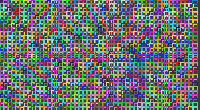
\includegraphics[width=0.99\linewidth]{figures/anchors/boxes_layers_1.png}
      \caption{Every possible boxes for anchor $5\times5$}
    \end{subfigure}
    \begin{subfigure}[t]{.49\linewidth}
      \centering
      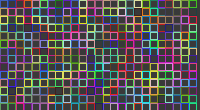
\includegraphics[width=0.99\linewidth]{figures/anchors/boxes_layers_2.png}
      \caption{Every possible boxes for anchor $7\times7$}
    \end{subfigure}
    \begin{subfigure}[t]{.49\linewidth}
      \centering
      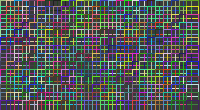
\includegraphics[width=0.99\linewidth]{figures/anchors/boxes_layers_3.png}
      \caption{Every possible boxes for anchor $12\times12$}
    \end{subfigure}
    \begin{subfigure}[t]{.49\linewidth}
      \centering
      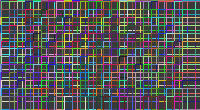
\includegraphics[width=0.99\linewidth]{figures/anchors/boxes_layers_4.png}
      \caption{Every possible boxes for anchor $21\times21$}
    \end{subfigure}
    \caption{Graphical representation of all the possible boxes that the network can predict, displayed per anchor. This illustration considers an input shape of $110\times200$ pixels, and the model architecture described in Table \ref{tab:nnstruct}.}
    \label{fig:anchors}
  \end{center}
\end{figure}


\subsection{Feature Extraction}
\paragraph{}

As we already discussed during Section \ref{Assumptions}, the traffic signs are made to be detected and are so very easy to capture. As you can see on Table \ref{tab:nnstruct} and Figure \ref{fig:nnstruct}, the features extraction layers is very limited compared to other lightweight models such as MobileNet \cite{sandler2018mobilenetv2}. With only five layers as a first feature extraction followed by three layers of higher order feature detection. This architecture allows reducing drastically the number of floating-point operation needed. Our model requires $39$ Millions floating-point operation (FLOP), while common architecture like tiny Yolo v3 \cite{yolov3} use $5,600$ Millions FLOP.

\begin{table}[]
    \centering
    \caption{Description of the neural network structure, block by block, giving the link between the blocks and some information such as the use Batch Normalization (BN) or residual connections (Res).}
    \begin{tabular}{|c|c|c|c|c|c|c|c|c|}
    \hline
    Name & Filter & Kernel & Stride & Activation & BN & Res & Input size & Input \\ \hline
    Conv1 & $8$ & $(3, 3)$ & $(2, 2)$ & ReLu6 & \checkmark &  & $(111, 201, 3)$ &  \\
    block\_0 & $8$ & $(3, 3)$ & $(1, 1)$ & ReLu6 & \checkmark & \checkmark & $(55, 100, 8)$ & Conv1 \\
    block\_1 & $16$ & $(3, 3)$ & $(2, 2)$ & ReLu6 & \checkmark &  & $(55, 100, 8)$ & block\_0 \\
    block\_2 & $16$ & $(3, 3)$ & $(1, 1)$ & ReLu6 & \checkmark & \checkmark & $(28, 50, 16)$ & block\_1 \\
    block\_3 & $16$ & $(3, 3)$ & $(1, 1)$ & ReLu6 & \checkmark & \checkmark & $(28, 50, 16)$ & block\_2 \\
    block\_4 & $16$ & $(3, 3)$ & $(2, 2)$ & ReLu6 & \checkmark &  & $(28, 50, 16)$ & block\_3 \\
    block\_5 & $16$ & $(3, 3)$ & $(1, 1)$ & ReLu6 & \checkmark & \checkmark & $(14, 25, 16)$ & block\_4 \\
    block\_6 & $16$ & $(3, 3)$ & $(1, 1)$ & ReLu6 & \checkmark & \checkmark & $(14, 25, 16)$ & block\_5 \\
    output\_1 & $2$ & $(3, 3)$ & $(1, 1)$ & Linear &  &  & $(28, 50, 16)$ & block\_3 \\
    output\_2 & $2$ & $(3, 3)$ & $(1, 1)$ & Linear &  &  & $(28, 50, 16)$ & block\_3 \\
    output\_3 & $2$ & $(3, 3)$ & $(1, 1)$ & Linear &  &  & $(14, 25, 16)$ & block\_6 \\
    output\_4 & $2$ & $(3, 3)$ & $(1, 1)$ & Linear &  &  & $(14, 25, 16)$ & block\_6 \\
    output\_5 & $2$ & $(3, 3)$ & $(1, 1)$ & Softmax &  &  & $(14, 25, 16)$ & block\_6 \\
    \hline
    \end{tabular}
    \label{tab:nnstruct}
\end{table}{}


\begin{table}[]
    \centering
    \caption{Activation area and associated anchors of each output layers}
    \begin{tabular}{|c|c|c|}
        \hline
        Layer & Anchors size & Activation area \\ \hline
        output\_1 & 3 & $24\times24$ \\
        output\_2 & 5 & $24\times24$ \\
        output\_3 & 7 & $56\times56$ \\
        output\_4 & 12 & $56\times56$ \\
        output\_5 & 21 & $56\times56$ \\
        \hline
    \end{tabular}
    \label{tab:activationArea}
\end{table}{}

\begin{figure}
    \centering
    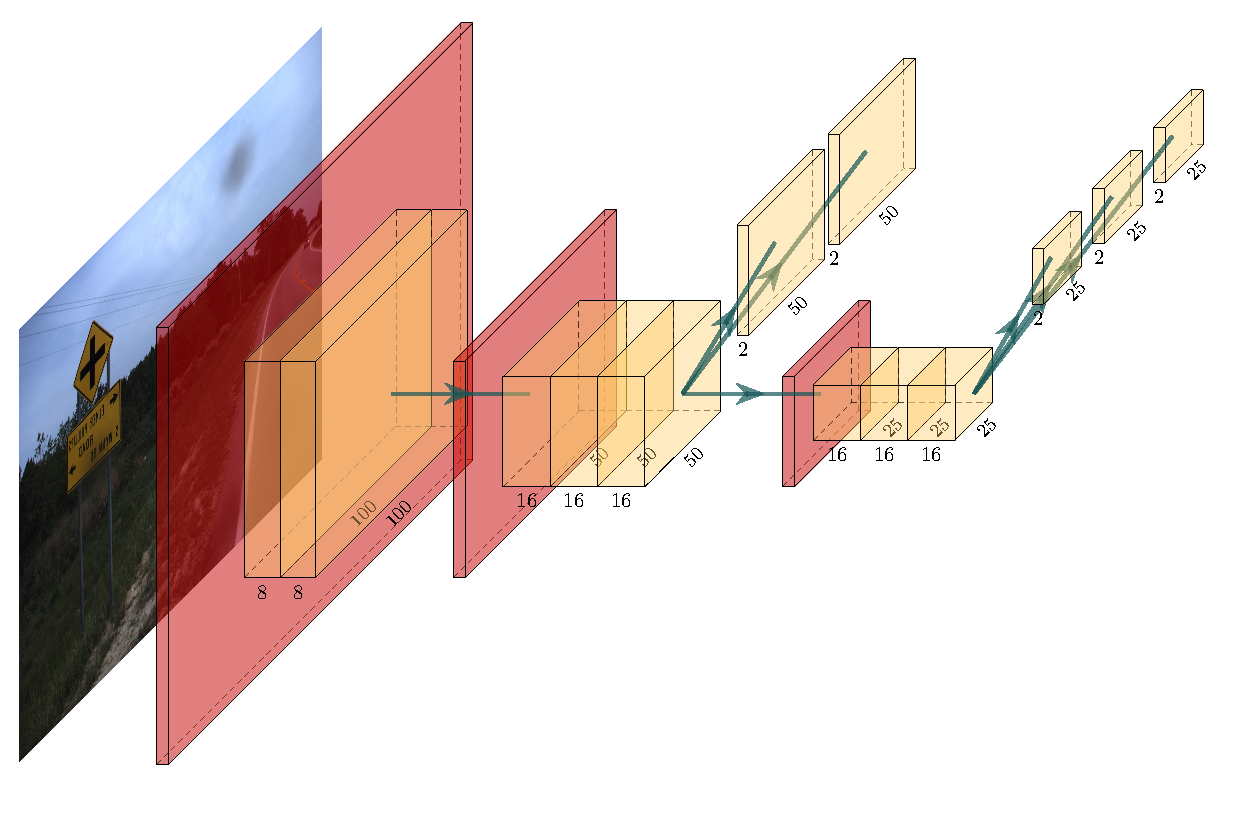
\includegraphics[width=\linewidth]{figures/my_arch}
    \caption{Structure of the neural network, orange boxes are convolution, red boxes indicate a stride 2 on the following layer}
    \label{fig:nnstruct}
\end{figure}{}

\section{Overfitting study} \label{sec:overfit}
\paragraph{}
A first basic check to verify if the model can learn something usefully is to try to overfit it on the data you have. If the model is not capable of overfitting them, then your model is not complex enough to understand the complexity of the data. The idea is that if the network is not able to give correct prediction on the training set, how can we expect it to give correct prediction on unseen data.

We performed this kind of study for the three different kind of block we consider here: inverted residual bottleneck, residual and convolution, as well as for three different set of filters size: $(32,64)$, $(16,24)$ and $(8,16)$. The first number representing the number of filters for Conv1 and Block 0, while the second number being the number of filters for block 1 to 6. Please refer to Table \ref{tab:nnstruct} for more information about those layers. All the block considered here are supposed to have similar expression potential, however, using different number of filters as a big impact on how much information the network can carry. On a general basis, the more filters the network has, the easier it will be to overfit the data.

To perform this analysis, we set the experiment in the following way. Aside from the parameters given previously, all the other meta parameters are set to same values across all test. The data augmentation is disabled, and the dropout is set to $0$. No early stopping strategy is used, and all network are trained for $200$ epochs on the full training split of the dataset, with a batch size of $128$.

\begin{figure}
  \begin{center}
    \begin{subfigure}[t]{.49\linewidth}
      \centering
      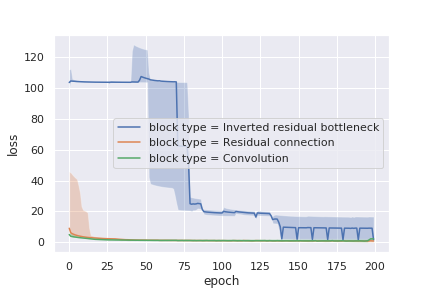
\includegraphics[width=0.99\linewidth]{figures/all_epoch_loss_block_type.png}
      \caption{Evolution of the training loss with epoch, for different block type}
      \label{fig:overfitloss}
    \end{subfigure}
    \begin{subfigure}[t]{.49\linewidth}
      \centering
      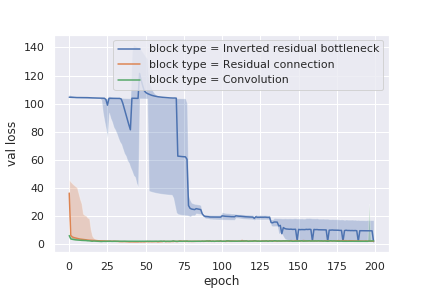
\includegraphics[width=0.99\linewidth]{figures/all_epoch_val_loss_block_type.png}
      \caption{Evolution of the validation loss with epoch, for different block type}
      \label{fig:overfitvalloss}
    \end{subfigure}
    \begin{subfigure}[t]{.49\linewidth}
      \centering
      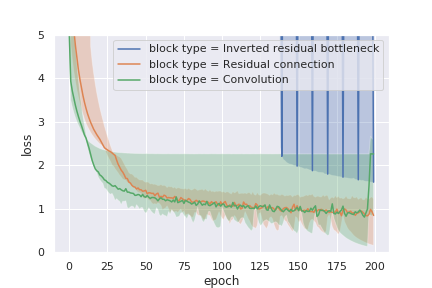
\includegraphics[width=0.99\linewidth]{figures/all_epoch_loss_block_type_zoomed_0_5.png}
      \caption{Evolution of the training loss with epoch, for different block type, zoomed on loss between 0 and 5}
      \label{fig:overfitloss_zoom}
    \end{subfigure}
    \begin{subfigure}[t]{.49\linewidth}
      \centering
      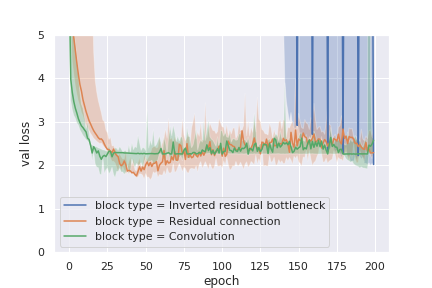
\includegraphics[width=0.99\linewidth]{figures/all_epoch_val_loss_block_type_zoomed_0_5.png}
      \caption{Evolution of the validation loss with epoch, for different block type, zoomed on loss between 0 and 5}
      \label{fig:overfitvalloss_zoom}
    \end{subfigure}
    \caption{Evolution of the validation and training loss for different block type, the hard line represent the median value, while the highlighted area go from the min to the max, for the different filters count.}
    \label{fig:overfit}
  \end{center}
\end{figure}

The training curve we get from this experiment are displayed on Figure \ref{fig:overfit}. You can see on Figure \ref{fig:overfitloss} and \ref{fig:overfitvalloss} that one block have lot of trouble learning anything. The inverted residual bottleneck block show very chaotic loss evolution, and never manage to overfit the data. As displayed on Figure \ref{fig:overfitloss_zoom}, the training loss of this block never reach $1.5$ in the given $200$ epochs. In the worst case, this block never get train loss better than $5$, while mAP@0.5 for loss over $3$ in this setup never crossing the bar of the $0.03$. On the other hand, Figure \ref{fig:overfitvalloss_zoom}, show that in this region of the graph the validation loss of the inverted residual bottleneck block in very consistent with the training loss, we are going to come back to that point latter.

The two other kinds of blocks, convolution and residual, behave in a similar manner. In both case their loss quickly drop to values around $2$ and overfitting start to appear. Overfitting is clearly visible for the residual block around epoch $40$ on Figure \ref{fig:overfitvalloss_zoom}. Both show that they successfully overfit the dataset, expect the case of the convolution block with the smaller filters, which did not manage to overfit the data, resulting in a steady loss at $2.3$, visible on Figure \ref{fig:overfitloss_zoom}.

\paragraph{}
The case of the inverted residual bottleneck block catch our attention, for multiple reason. First, the case getting the best results is not the one with the higher number of filters as one could expect, but the one with the smallest number of filters. In addition, even with all the trick supposed to prevent overfitting disabled, the network still did not overfit and get consistently decreasing training and validation loss. We decided to train it further, running for $600$ with some data augmentation and dropout to prevent overfitting. The evolution of the loss can be seen on Figure \ref{fig:mn600}. You can see that as previously, in Figure \ref{fig:overfit}, this model as a strange behavior during the first epochs, until a point where the loss start dropping in a more usual fashion. Training could have been performed for a longer time as the loss was still decreasing, but that first exploration showed encouraging results with an mAP@50 reaching $0.4$. However, as you can see on figure \ref{fig:overfitmAP}, this mAP level on the validation set is reached by all the different block even when trying to overfit them on the training data.

\begin{figure}
  \begin{center}
    \begin{subfigure}[t]{.49\linewidth}
      \centering
      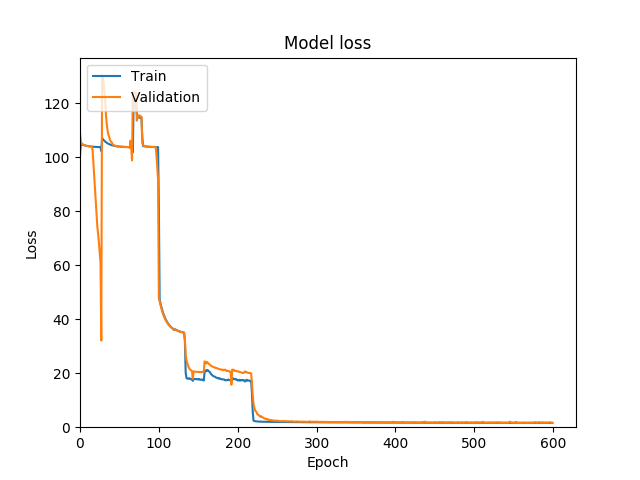
\includegraphics[width=0.99\linewidth]{figures/nNetloss_mn_816_600.png}
      \caption{Evolution of the loss with epochs}
      \label{fig:mn600loss}
    \end{subfigure}
    \begin{subfigure}[t]{.49\linewidth}
      \centering
      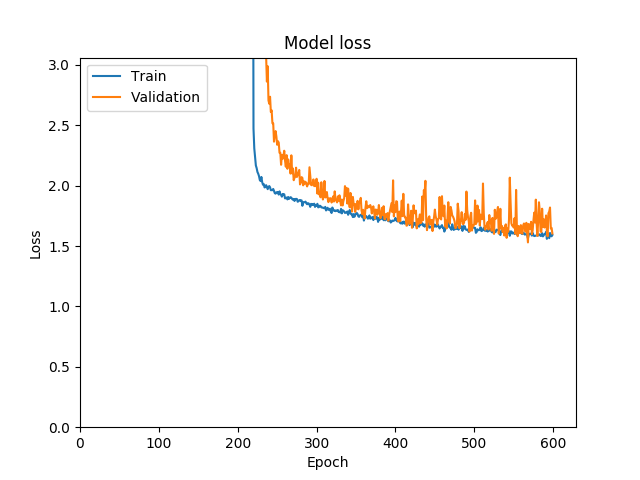
\includegraphics[width=0.99\linewidth]{figures/nNetloss_mn_816_600_zoomed.png}
      \caption{Evolution of the loss with epochs, zoomed on y axis}
      \label{fig:mn600lossZoomed}
    \end{subfigure}
    \caption{Evolution of the validation and training loss during training for an inverted residual bottleneck block type model, trained over $600$ epochs.}
    \label{fig:mn600}
  \end{center}
\end{figure}

\begin{figure}
    \centering
    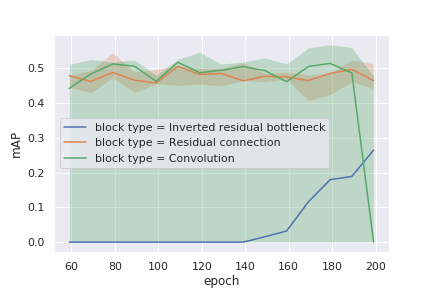
\includegraphics[width=.5\linewidth]{figures/all_epoch_mAP_block_type.png}
    \caption{Evolution of the mAP@50 on validation set for the different blocks type during the overfiting study.}
    \label{fig:overfitmAP}
\end{figure}{}

\paragraph{}
From this study we concluded that the inverted residual bottleneck can be difficult to train and does not provide better accuracy than what the other block propose. In the other hand as expected convolution and residual convolution perform in a quite similar way as expected, with the residual version looking more stable even if slower to train. From these results we chose to focus our efforts toward the residual block, discard any more exploration on the convolutions block, and keep the inverted residual bottleneck as a comparison for the rest of the study.

\section{Pretraining}
\paragraph{}
Study of the weights trained during Section \ref{sec:overfit} showed that the trained network were still performing in a sub-optimal fashion. Weights of the first layer filters were still very noisy and no matter the training strategy used remained so. If they still have interest on yellow objects, most of them were still random and very far from the edge detector filters one would expect from a properly trained network.

The most common way to solve that issue is to have more data for training. When having more training samples is not an option, the usual way is to pretrain the model on one of the public dataset, such as ImageNet \cite{deng2009imagenet} or Cifar \cite{krizhevsky2009cifar10}. But if such a strategy have been proven to be successful to get good generic first filters and if this method would probably have been successful in this study too, the filters would have been generic and so not as efficient as possible for this task, resulting in more filters than necessary. Our main goal being to target efficiency we chose another approach to that problem. As already described in Section \ref{sec:dataGen}, we chose to generate new artificial data to train the network on a similar task.

For this new task, being easier and virtually having unlimited data available, it was easy to achieve over $0.8$ mAP@50 on this set of data with all the different models. Using this trained weights for fine-tuning on real world data, successfully boosted the accuracy of our model, adding from $0.1$ to $0.2$ to the final mAP, as you can see on Table \ref{tab:mapFineTuning}. This Table compare different models, with different filters, each described by a tuple of two numbers. The first representing the number of
filters for Conv1 and Block 0, while the second being the number of filters for block 1 to 6. The Table compare the models for two different intersection over union thresholds, $25\%$ and $50\%$, to give a better idea of there localization accuracy, and give the relative improvement obtained by training first on the artificial data before fine-tuning on the real cases. For each model the same meta parameters were used during training. In the direct training case, the models were trained for $600$ epochs on the real data starting with random weights with an initial learning rate of $0.01$. In the fine-tuning case, the models were first trained for $200$ epochs on the artificial data, with an initial learning rate of $0.01$, and these weights were then used for training for $600$ epochs on the real world data with a smaller initial learning rate of $0.001$. Table \ref{tab:mapFineTuning} clearly show that using the artificially generated data provide a large improvement in accuracy as well as allowed to stabilize the training process preventing case like the residual model with filters $(16,24)$ not being able to learn anything over the training. As previously experienced during this study, the inverted residual bottleneck also behave here strangely. If once again we cannot say that this layer is not working, initializing the weights on the artificial data did not bring any improvements and even make results worst.

\begin{table}[]
    \centering
    \caption{Summary of the evolution of the mAP with and without fine turning. Direct training values are get after training random weights on the real word annotation, while Fine tuning are get by first training the weights on artificial data.}
    \begin{tabular}{|c|c|c|c|c|c|c|c|}
        \hline
        \multirow{3}{*}{Block type} & \multirow{3}{*}{Filters} & \multicolumn{4}{|c|}{mAP} & \multicolumn{2}{|c|}{\multirow{2}{*}{Improvement}} \\
        & & \multicolumn{2}{|c|}{Direct Training} & \multicolumn{2}{|c|}{Fine tuning} & \multicolumn{2}{|c|}{}\\ 
        & & @25 & @50 & @25 & @50 & @25 & @50 \\ \hline
        \multirow{3}{*}{Residual} & $(8,16)$   & $0.58$ & $0.45$ & $0.68$ & $0.55$ & $+17.2\%$ &                               $+22.2\%$ \\
                                  & $(16,24)$ & $0.00$ & $0.00$ & $0.73$ & $0.61$ & $+\infty$ & $+\infty$ \\
                                  & $(32,64)$ & $0.62$ & $0.52$ & $0.82$ & $0.67$ & $+32.3\%$ & $+28.8\%$ \\ \hline
        Inverted Residual         & $(8,16)$   & $0.49$ & $0.38$ & $0.43$ & $0.30$ & $-12.24\%$ &                               $-21.05\%$\\ \hline
    \end{tabular}
    \label{tab:mapFineTuning}
\end{table}


As you can see the accuracy vary a lot from one model to the other, but as always in this study, it is always a matter of trade of. More filters mean more computation done which, on mobile device, automatically results in higher latency. With a previous demonstration of that showed on Figure \ref{fig:latencysize}, where you can see that the latency is directly linked to the input size, showing the importance of the meta parameters in the final detection speed.

\section{Latency study}
\paragraph{}
Speed is the ultimate target of this study, it has been under all the assumption and decision we took, but so far we barely discussed or gave results to asses these choices. The goal of this section is to expose the parameters having the more importance for over detection speed in our model and how they also affect accuracy. We are going here to cover the more important one, such as filter size and block type, input size being already discussed in Section \ref{sec:inputSize}.

\begin{figure}
  \begin{center}
    \begin{subfigure}[t]{.49\linewidth}
      \centering
      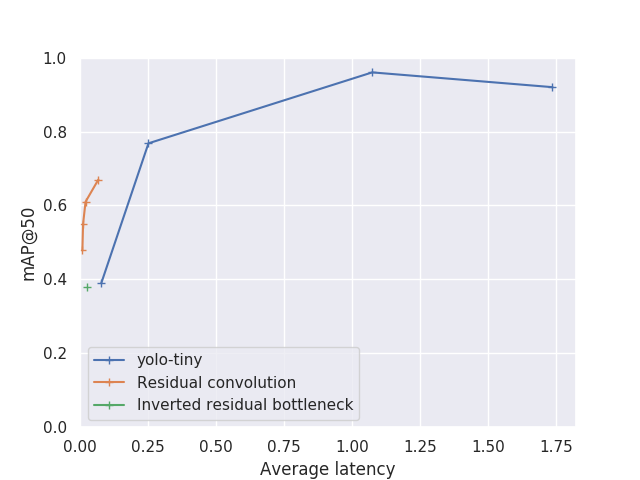
\includegraphics[width=0.99\linewidth]{figures/map_at_50_latency_models.png}
      \caption{Evolution of the mAP@50 with the latency}
    \end{subfigure}
    \begin{subfigure}[t]{.49\linewidth}
      \centering
      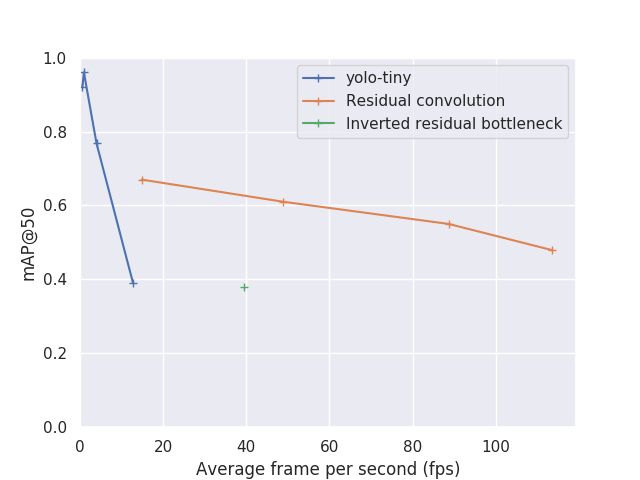
\includegraphics[width=0.99\linewidth]{figures/map_at_50_fps_models.png}
      \caption{Evolution of the mAP@50 with the frame per second}
    \end{subfigure}
    \begin{subfigure}[t]{.49\linewidth}
      \centering
      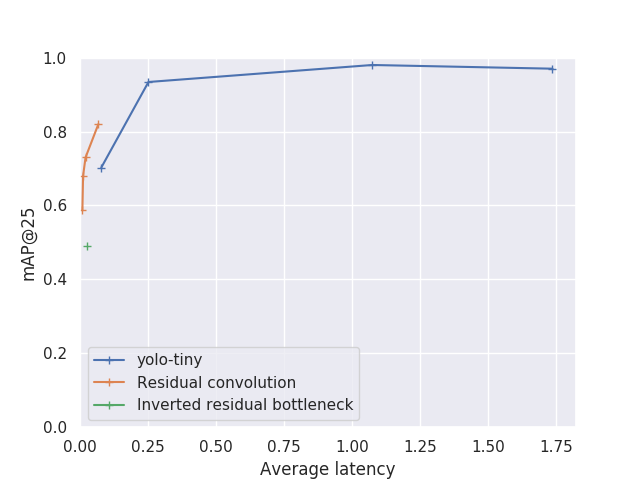
\includegraphics[width=0.99\linewidth]{figures/map_at_25_latency_models.png}
      \caption{Evolution of the mAP@25 with the latency}
    \end{subfigure}
    \begin{subfigure}[t]{.49\linewidth}
      \centering
      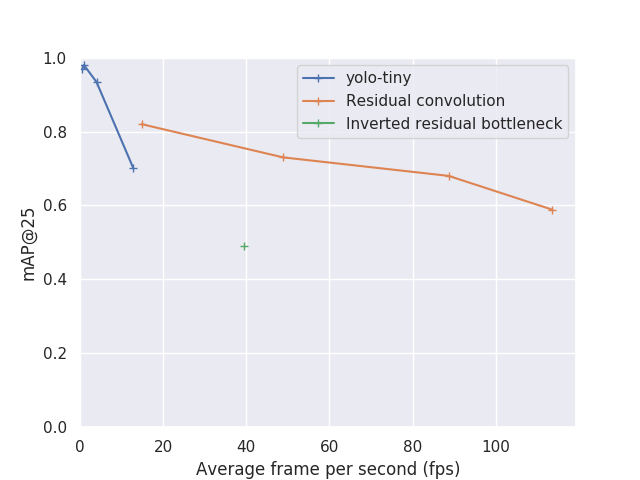
\includegraphics[width=0.99\linewidth]{figures/map_at_25_fps_models.png}
      \caption{Evolution of the mAP@25 with the frame per second}
    \end{subfigure}
    \caption{Plots of the ratio computation speed vs accuracy for different architectures, the residual block studied here and Yolov3-tiny, converted to TensorFlow lite with the code from \cite{benjamintanweihao2018Oct}. Speed are computed for a run on a Samsung S6 (SM-920T) using one thread.}
    \label{fig:map_to_speed}
  \end{center}
\end{figure}

\begin{table}[]
    \centering
    \caption{Value of the mAP, latency and frame per second for different configuration and different models. Numerical values used for the graphical representation of Figure \ref{fig:map_to_speed}}
    \begin{tabular}{|c|c|c|c|c|c|d{1}|}
        \hline
        Architecture & Input size & Filters & mAP@50 & mAP@25 & Latency (s) & \mathrm{FPS} \\ \hline
        \multirow{ 4 }{*}{ Yolov3-tiny } & 704x416 & - & 0.92 & 0.97 & 1.738 & 0.6 \\
    	  & 576x320 & - & 0.96 & 0.98 & 1.075 & 0.9 \\
    	  & 160x288 & - & 0.77 & 0.93 & 0.252 & 4.0 \\
    	  & 96x160  & - & 0.39 & 0.70 & 0.078 & 12.8 \\
    	\hline
    	\multirow{ 4 }{*}{ \shortstack{Residual\\convolution} } & 110x200 & (6,10) & 0.48 & 0.59 & 0.009 & 113.7 \\
    	  & 110x200 & (8,16) & 0.55 & 0.68 & 0.011 & 88.7 \\
    	  & 110x200 & (16,24) & 0.61 & 0.73 & 0.020 & 48.9 \\
    	  & 110x200 & (32,64) & 0.67 & 0.82 & 0.068 & 14.8 \\
    	\hline
    	Inverted & & & & & & \\
    	residual & 110x200 & (8,16) & 0.38 & 0.49 & 0.025 & 39.4 \\
    	bottleneck & & & & & & \\
    	\hline
    \end{tabular}
    \label{tab:map_to_speed}
\end{table}{}

Figure \ref{fig:map_to_speed} and Table \ref{tab:map_to_speed} show the evolution of the prediction speed on a mobile device and how the accuracy evolve with it. We also added values for Yolo v3 in its tiny version, as a comparison. The mAP value used in these graphs are the one get from the best training over all the combination we tried. The first thing to notice from this Figure, is the behavior of the inverted residual bottleneck. Speed is not even on the side of this block structure, that in addition to perform poorly is slower than is counterpart with the same amount of filters. Yolo, on another hand perform quite well on this task even on low resolutions. With an input size of $160\times288$ it reach a speed of $4fps$ while maintaining an mAP@50 of $77\%$. This speed is still too slow to be considered real time on a smartphone, but considering the accuracy it is still quite a good performance. But Yolo fail to reach higher speed as it is limited by its deep architecture. As you can see on Figure \ref{fig:map_to_speed}, its accuracy drop when trying to reach speed of $13fps$, with an input resolution of $96\times160$. Our architecture, with the residual convolution block and different filter size never manage to do better than $70\%$ of mAP@50 and has trouble to reach $80\%$ of mAP@25. However, as you will see on section \ref{sec:test}, this lower mAP is not really significant in real live use case. On the other side, our architecture, is able to maintain a good accuracy while decreasing the latency to extremely low level, allowing to run image object detection on a single thread of a smartphone faster than most camera are able to collect the images, leaving plenty of resource available to run other task simultaneously or simply saving energy and allowing longer battery live. Our fastest accurate model achieve $55\%$ mAP@50 and $68\%$ mAP@25 while running at $88fps$ on our test smartphone, a four years old model. The gap between mAP@50 and mAP@25 show that our model is however not very accurate in the localization of the object, but that was one of our core starting assumptions in Chapter \ref{chapter:technicalApproach} Section \ref{Assumptions}.

If our model manage to get good results, these results are evaluated according to a single metric, even if this metric is the reference in object detection filed, it is not perfect. In addition, if the validation data used to compute these values are never seen during training by the model, they came from the same set of data and so may have the same diversity, missing the same complex cases. It is so very important to conduce a more complete set of testing, in order to get a validation of the results we get previously.

\section{Testing results} \label{sec:test}
\subsection{Introduction}
\paragraph{}
In this section we are going to present the results of test we conduced on different set of data. This data were not annotated, preventing us to produce numbering such as mAP or any other metric. Our goal here is so more to represent how our model is performing in the wild, on real use cases. We are so going to present example of detection on different kind of road, with different traffic sign quality.

In this section we are going to review the results of one model. We chose here to evaluate the model based on residual convolution and with filters $(8,16)$, as it provide a very high processing speed, reaching $88fps$, while maintaining a good accuracy as you can see on Table \ref{tab:map_to_speed}. Our goal here is to illustrate what a low mAP mean on this model.

Because this section is a test, it is important to stress that our training data does not have any images took on these roads, and so they appear completely new to our algorithm. Also, as it is a final test, we did not to tune our model to improve the results, this is the final results after defining our model on the training and validation set. Some tuning will definitely improve the results, but will make it less close to a real use case we are simulating here.

\subsection{State Road 2} \label{sec:sr2}
\subsubsection{Presentation}
\paragraph{}
State road 2, in Georgia is one of the main testing site of our team. Figure \ref{fig:map_sr2} show the map of the section used for testing. This section of 21km (13 miles), have been chosen for it is high density of curve, resulting in a high density of warning sign in the area.

\begin{figure}
    \centering
    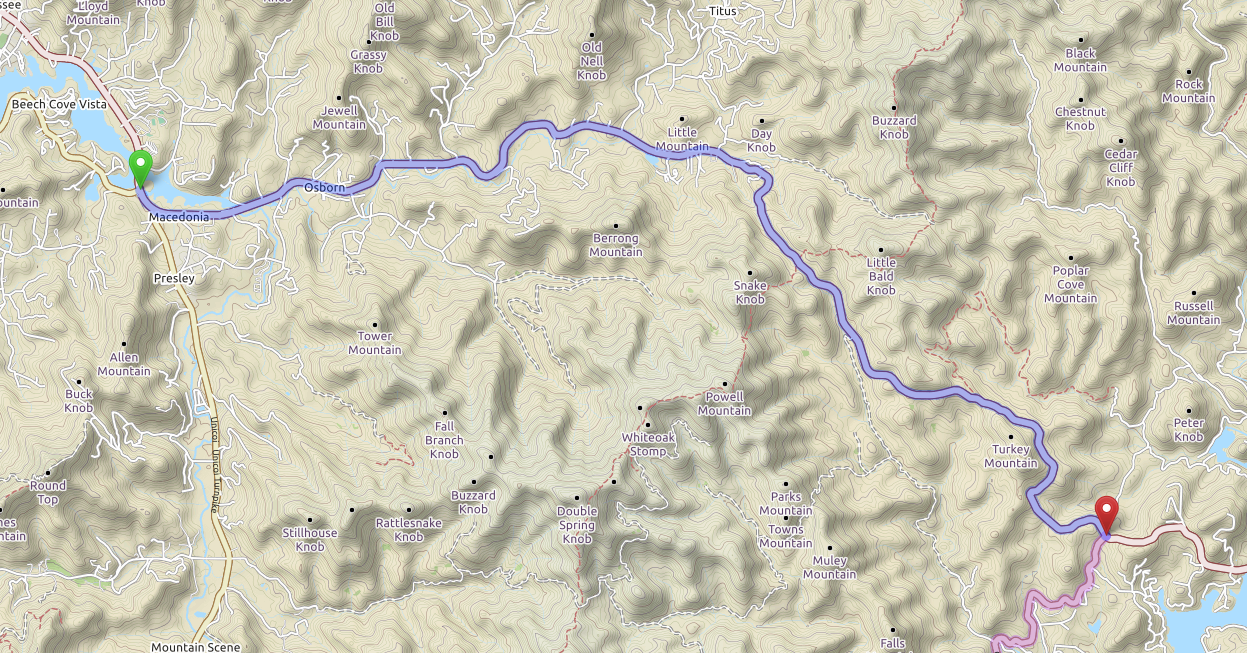
\includegraphics[width=0.8\linewidth]{figures/map_sr2.png}
    \caption{Map representing the test section we used on State Road 2}
    \label{fig:map_sr2}
\end{figure}{}

Being a state road, this area receive more care from the Department Of Transportation (DOT) than other areas, resulting on signs that are in better condition and are generally not obstructed by trees. In total there is more than one hundred signs on this section. From all the $70,438$ on which the model was run, and we reviewed we collected some interesting examples for each category that we are going to display bellow.

\subsubsection{False Positive cases}

\begin{figure}
  \begin{center}
    \begin{subfigure}[t]{.49\linewidth}
      \centering
      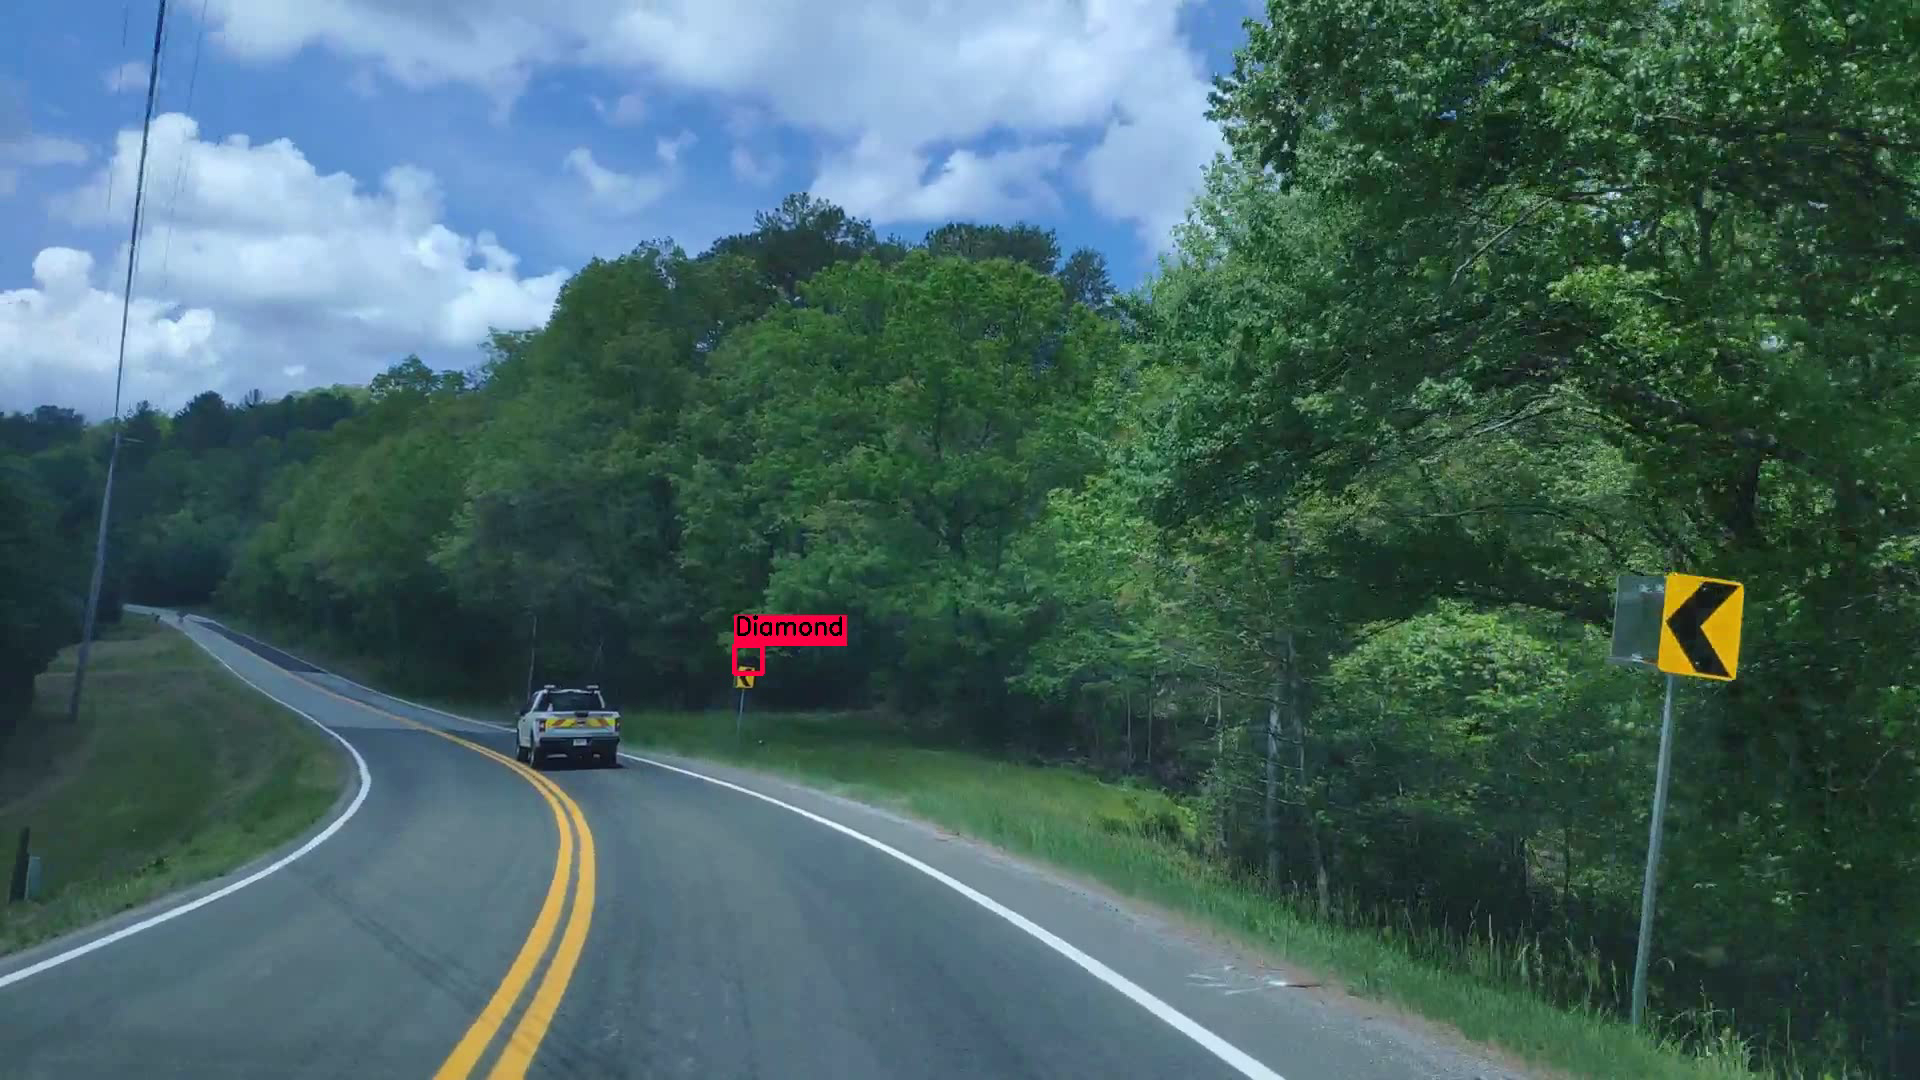
\includegraphics[width=0.99\linewidth]{figures/examples/sr2/FP/FP_13.png}
      \caption{Chevron Sign}
      \label{fig:chevronFP}
    \end{subfigure}
    \begin{subfigure}[t]{.49\linewidth}
      \centering
      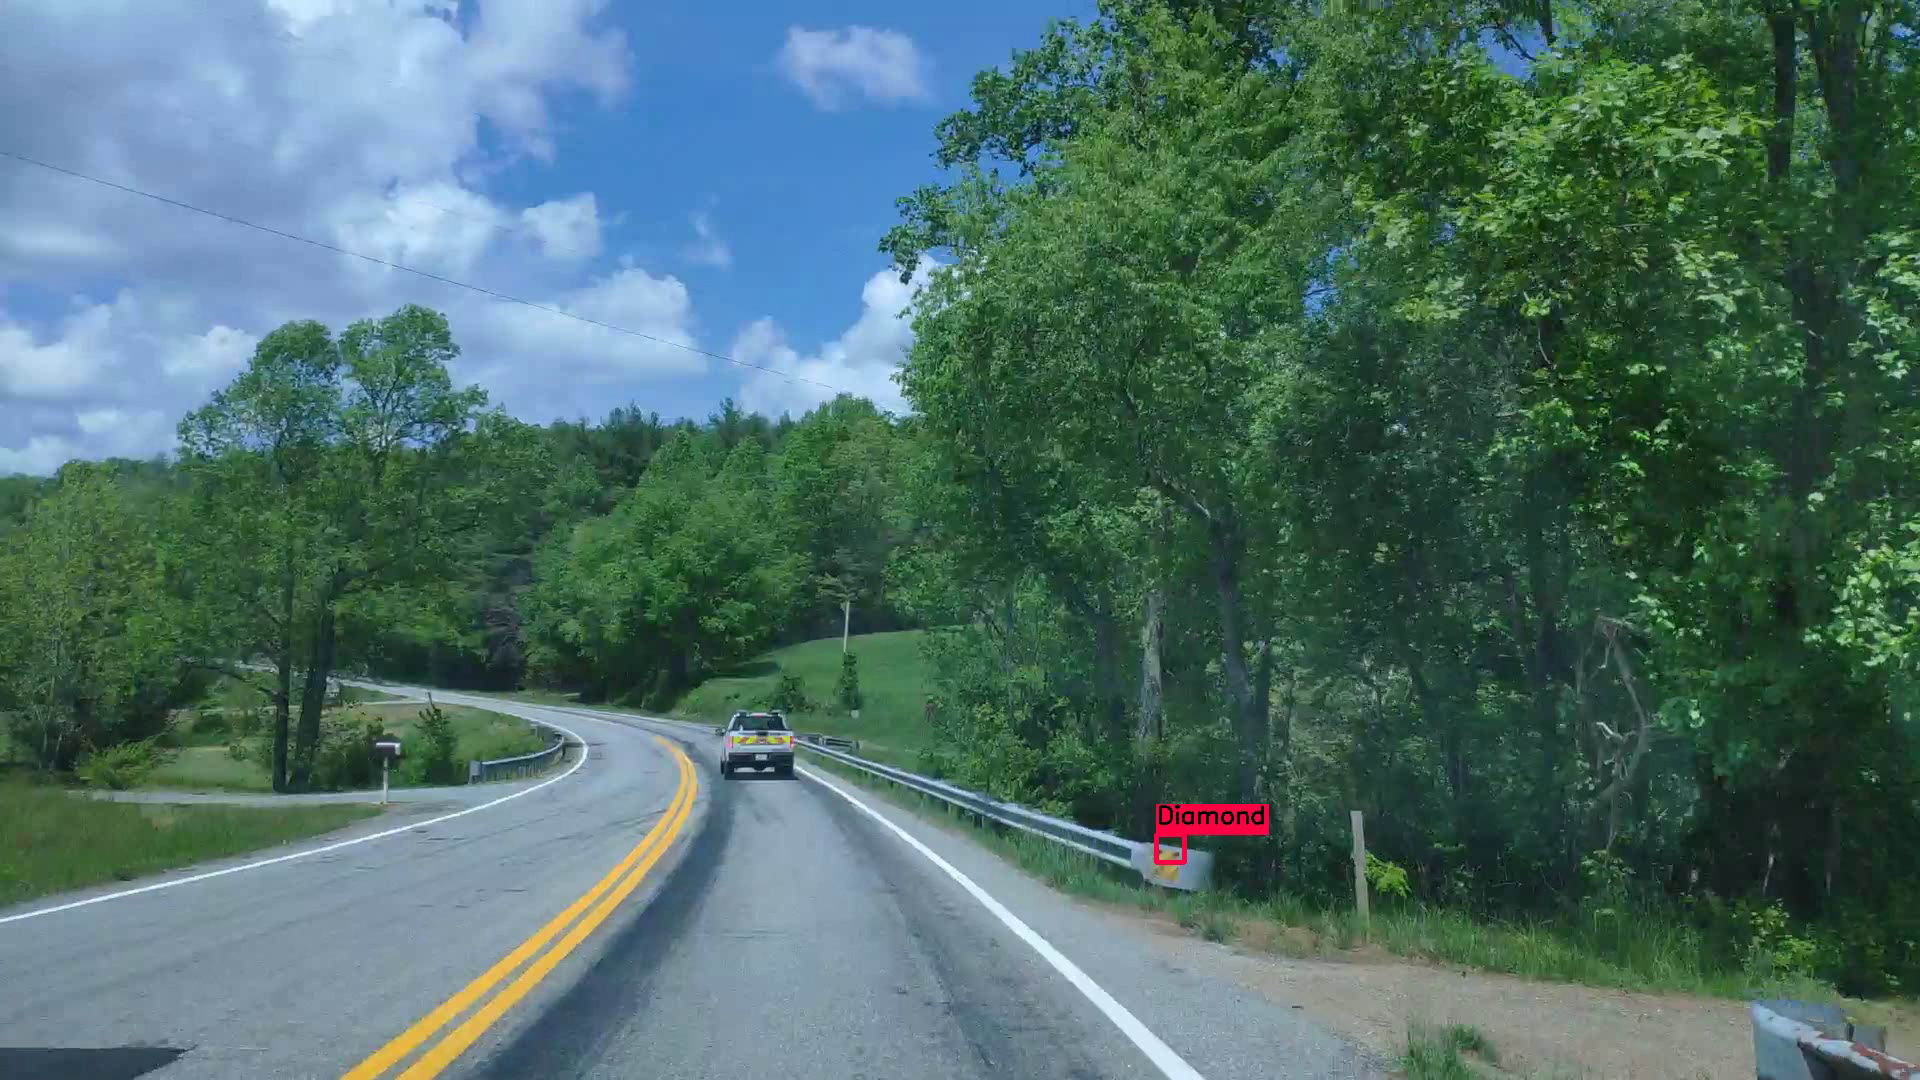
\includegraphics[width=0.99\linewidth]{figures/examples/sr2/FP/FP_09.png}
      \caption{Guard rail signalization}
      \label{fig:guardRailFP}
    \end{subfigure}
    \begin{subfigure}[t]{.49\linewidth}
      \centering
      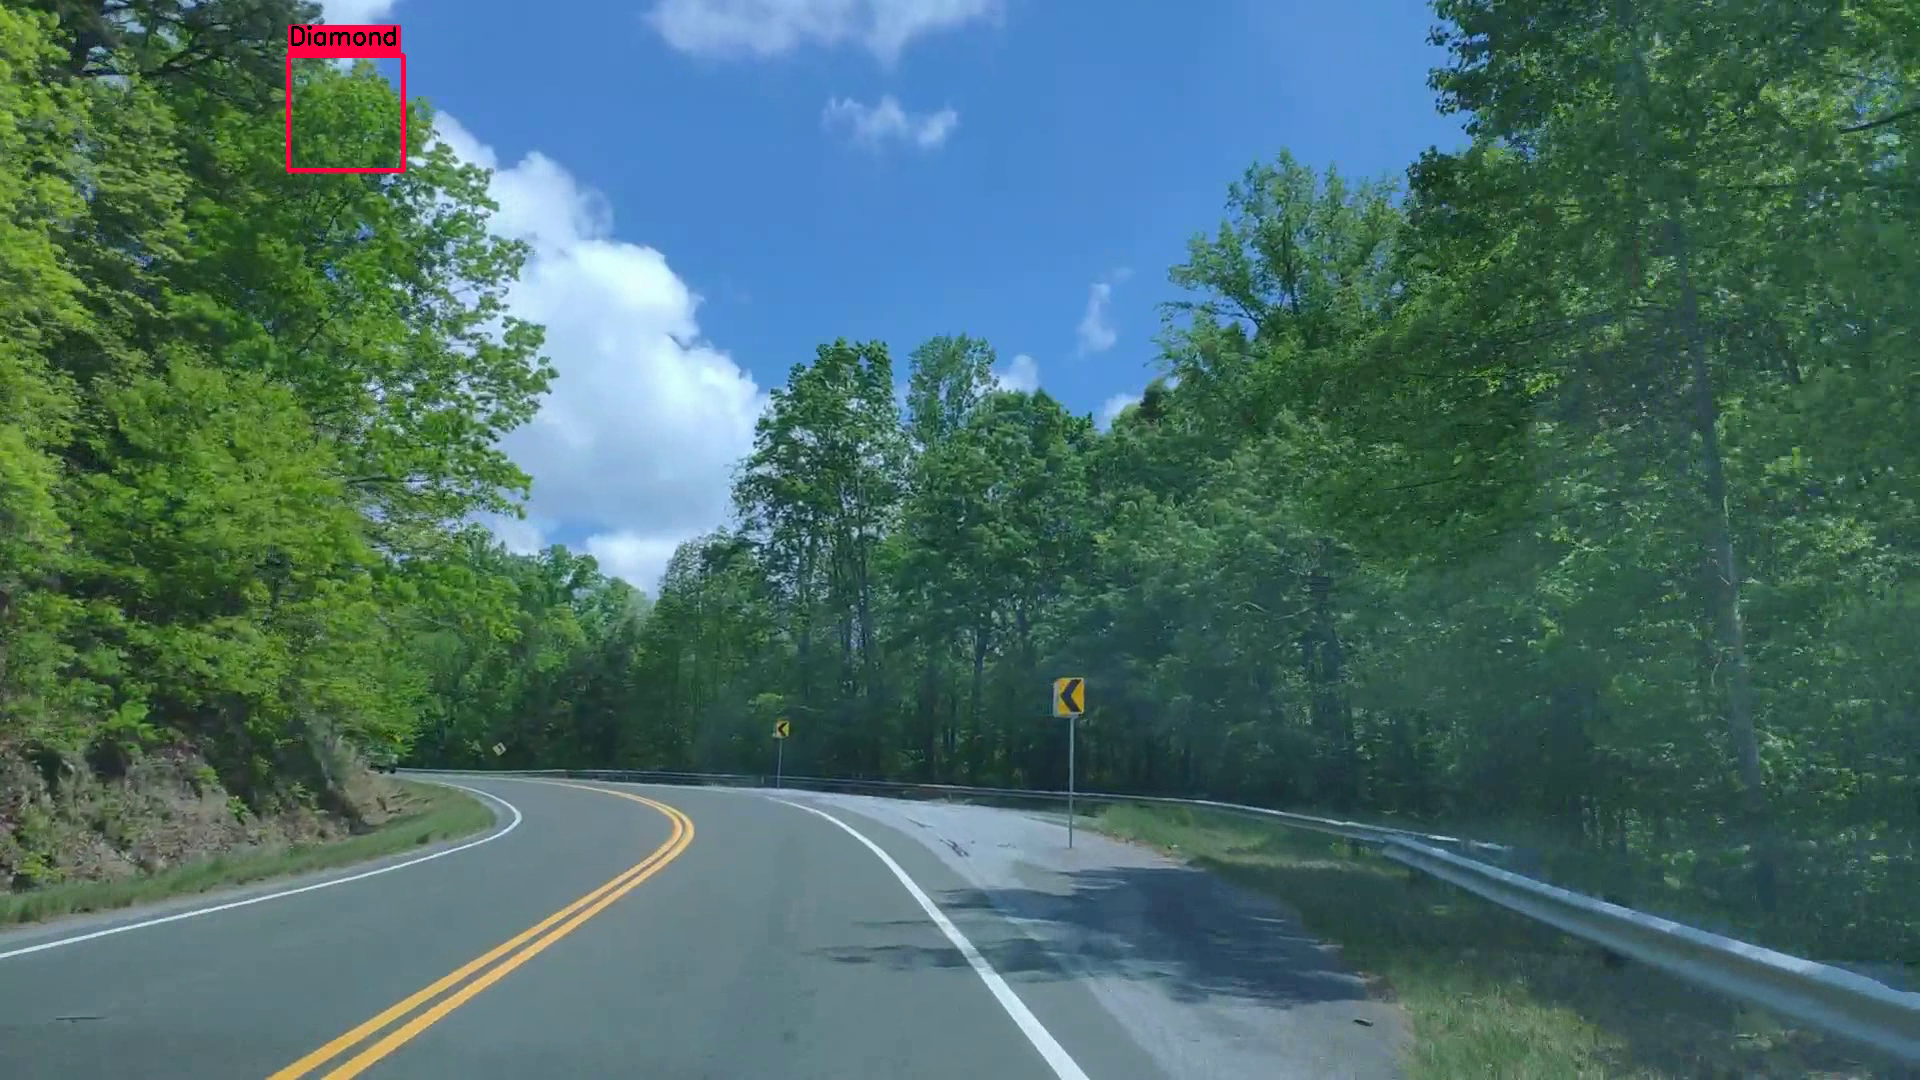
\includegraphics[width=0.99\linewidth]{figures/examples/sr2/FP/FP_04.png}
      \caption{Plants}
      \label{fig:plantFP}
    \end{subfigure}
    \begin{subfigure}[t]{.49\linewidth}
      \centering
      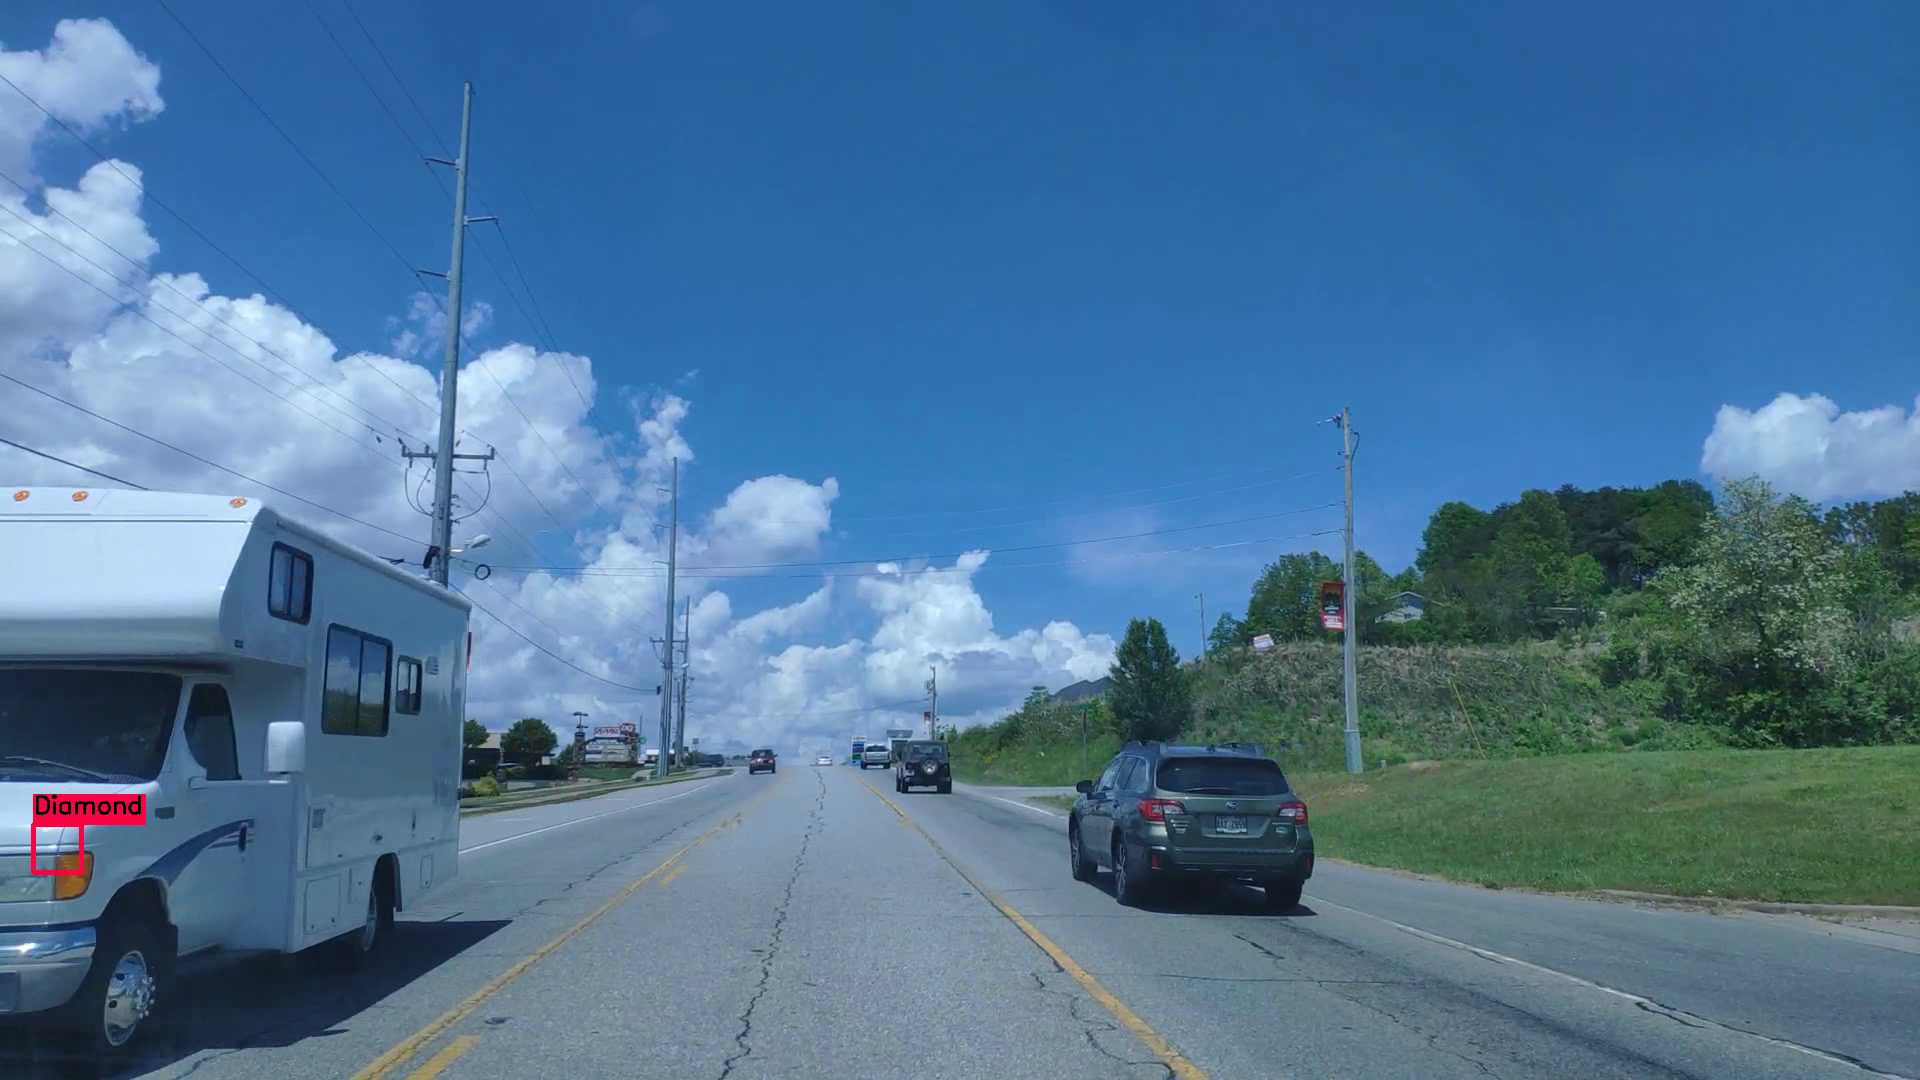
\includegraphics[width=0.99\linewidth]{figures/examples/sr2/FP/FP_19.png}
      \caption{Car Light}
      \label{fig:carLightFP}
    \end{subfigure}
    \begin{subfigure}[t]{.49\linewidth}
      \centering
      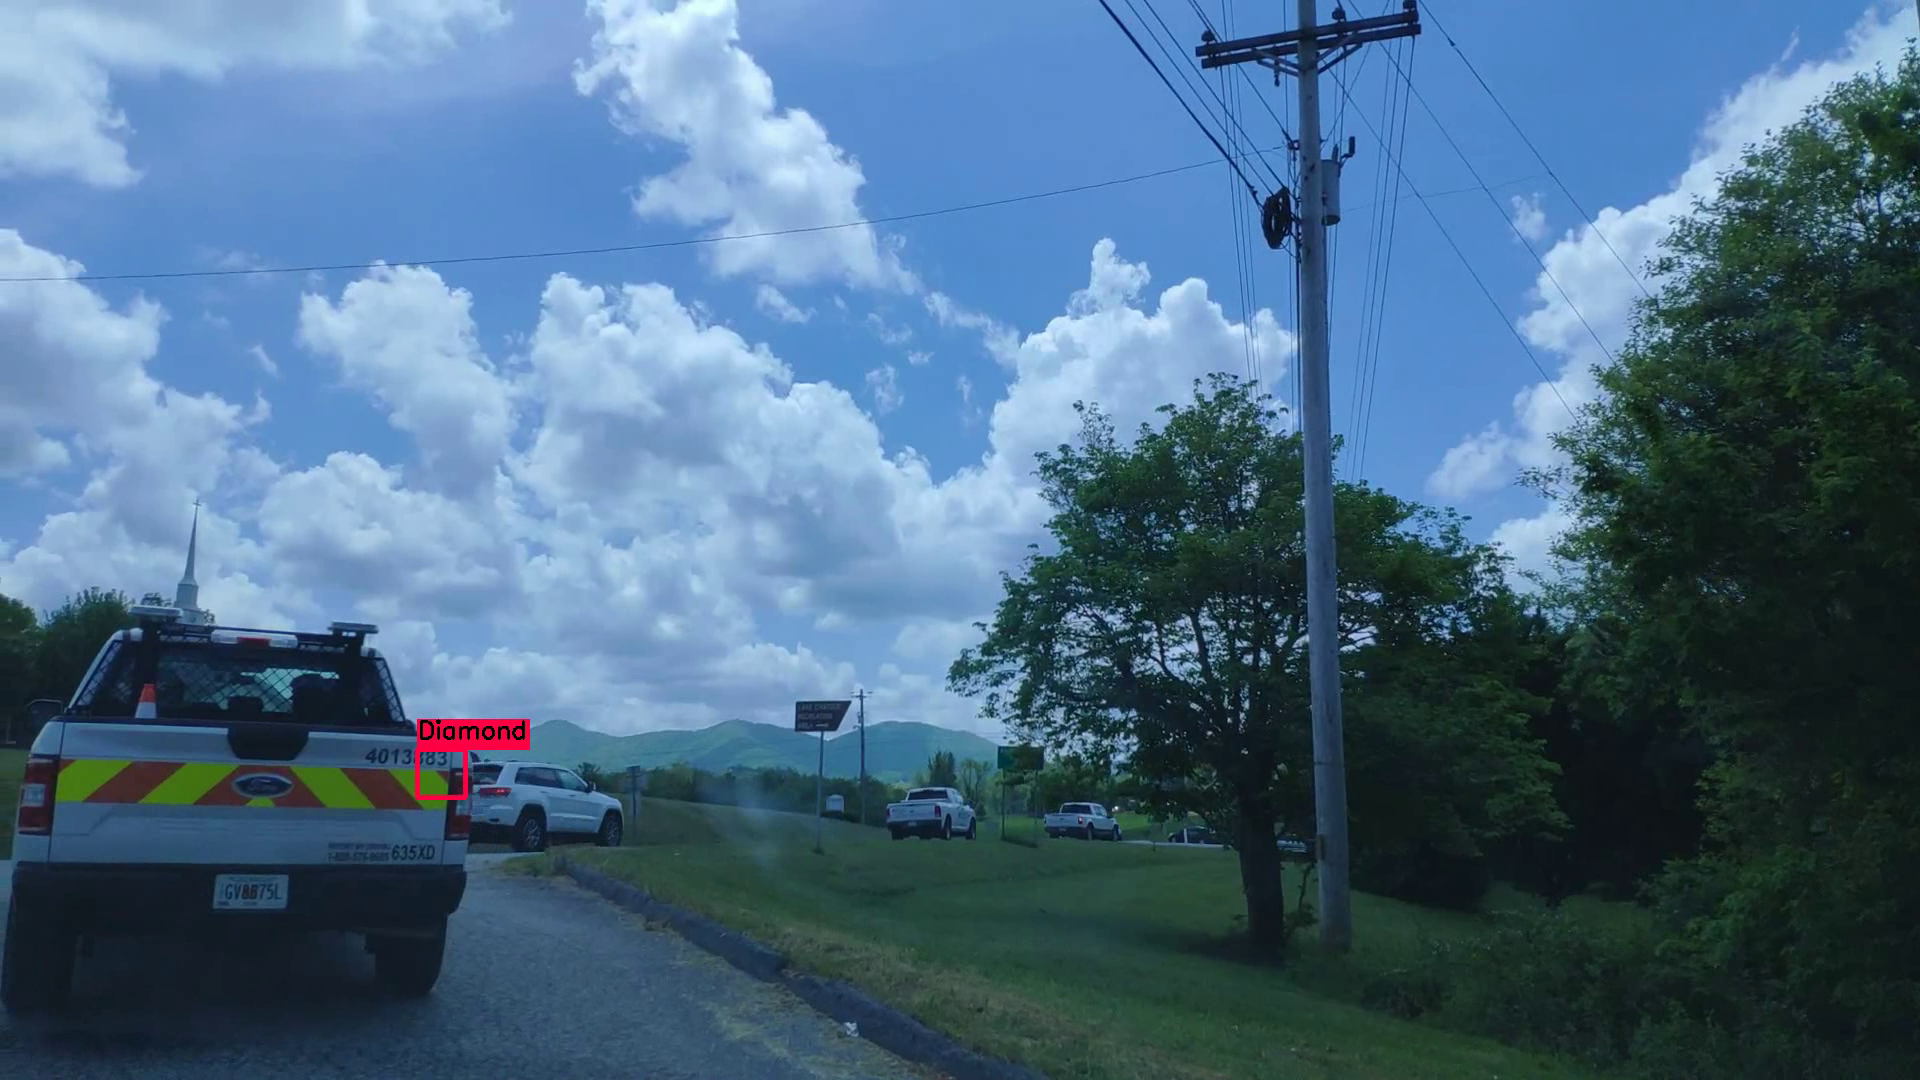
\includegraphics[width=0.99\linewidth]{figures/examples/sr2/FP/FP_01.png}
      \caption{Yellow signalization}
      \label{fig:GDOTtruckFP}
    \end{subfigure}
    \begin{subfigure}[t]{.49\linewidth}
      \centering
      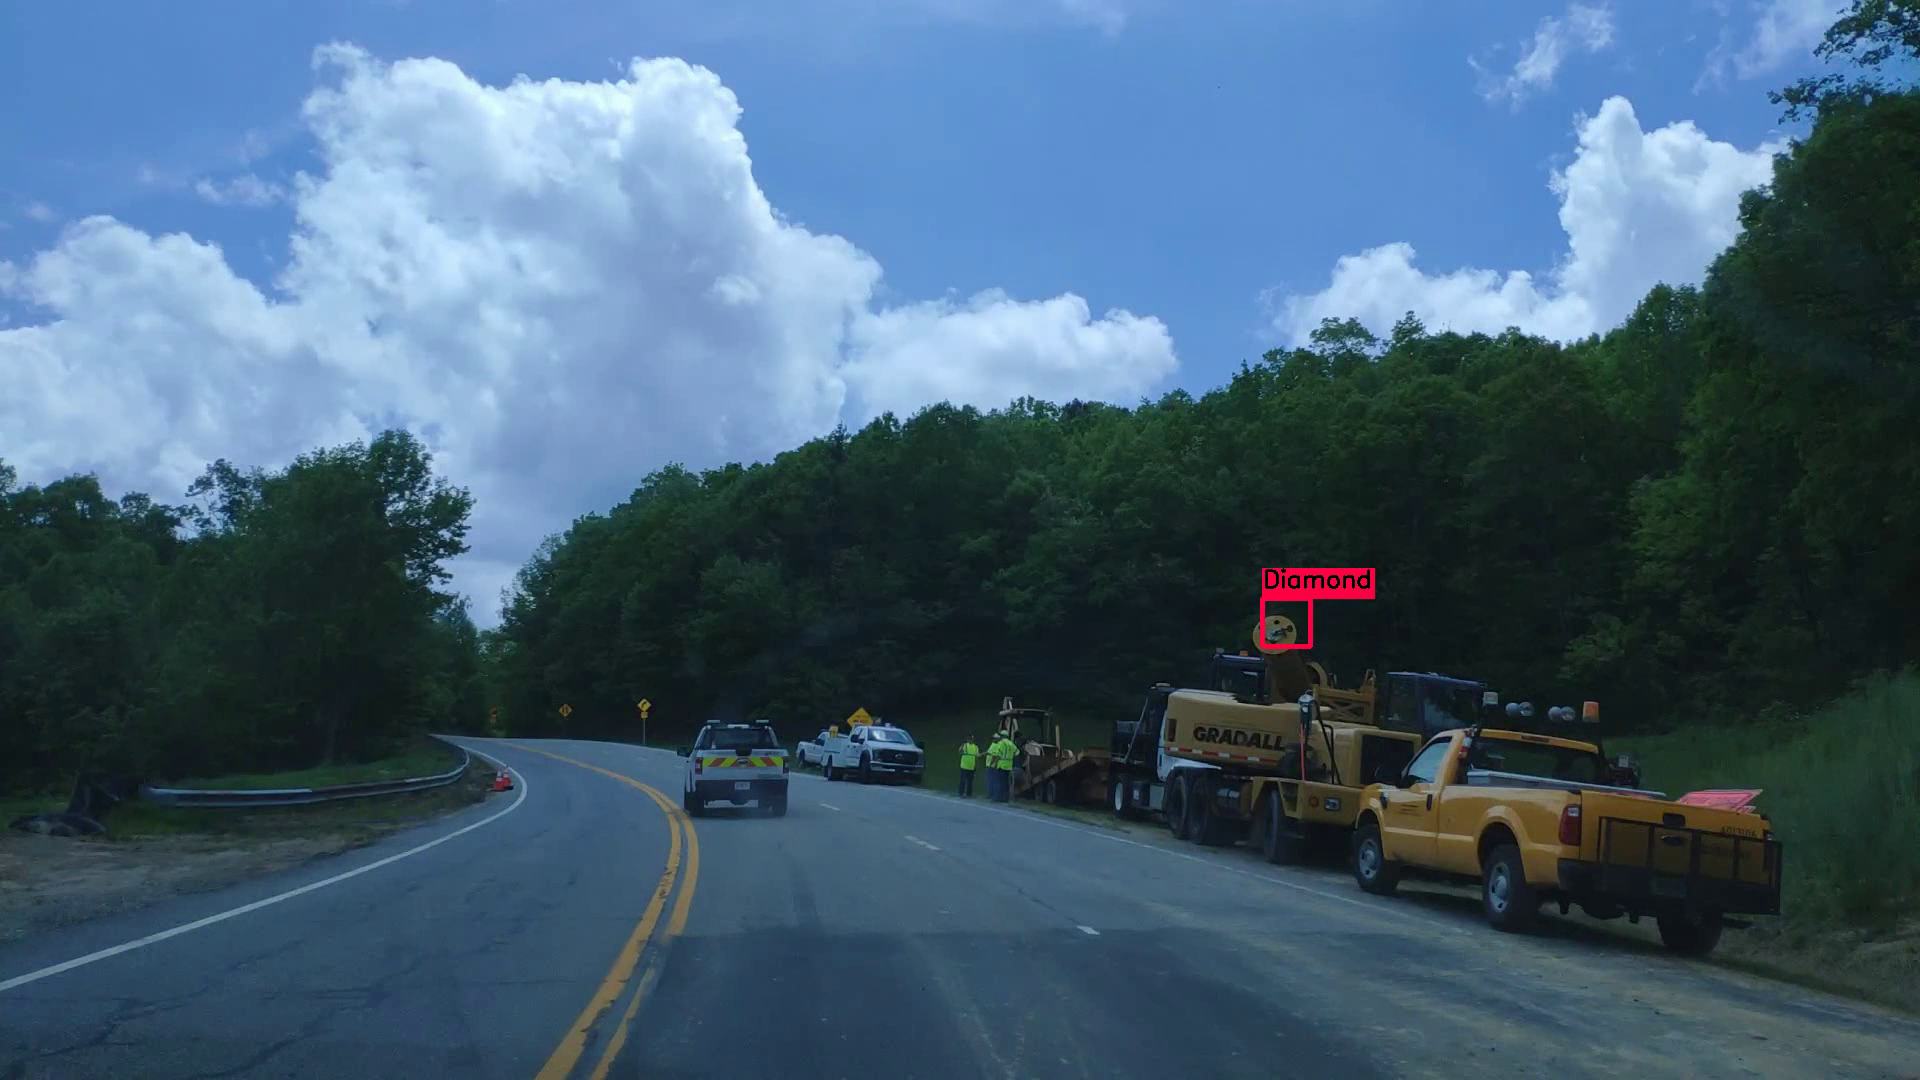
\includegraphics[width=0.99\linewidth]{figures/examples/sr2/FP/FP_03.png}
      \caption{Yellow digger}
      \label{fig:diggerFP}
    \end{subfigure}
    \begin{subfigure}[t]{.49\linewidth}
      \centering
      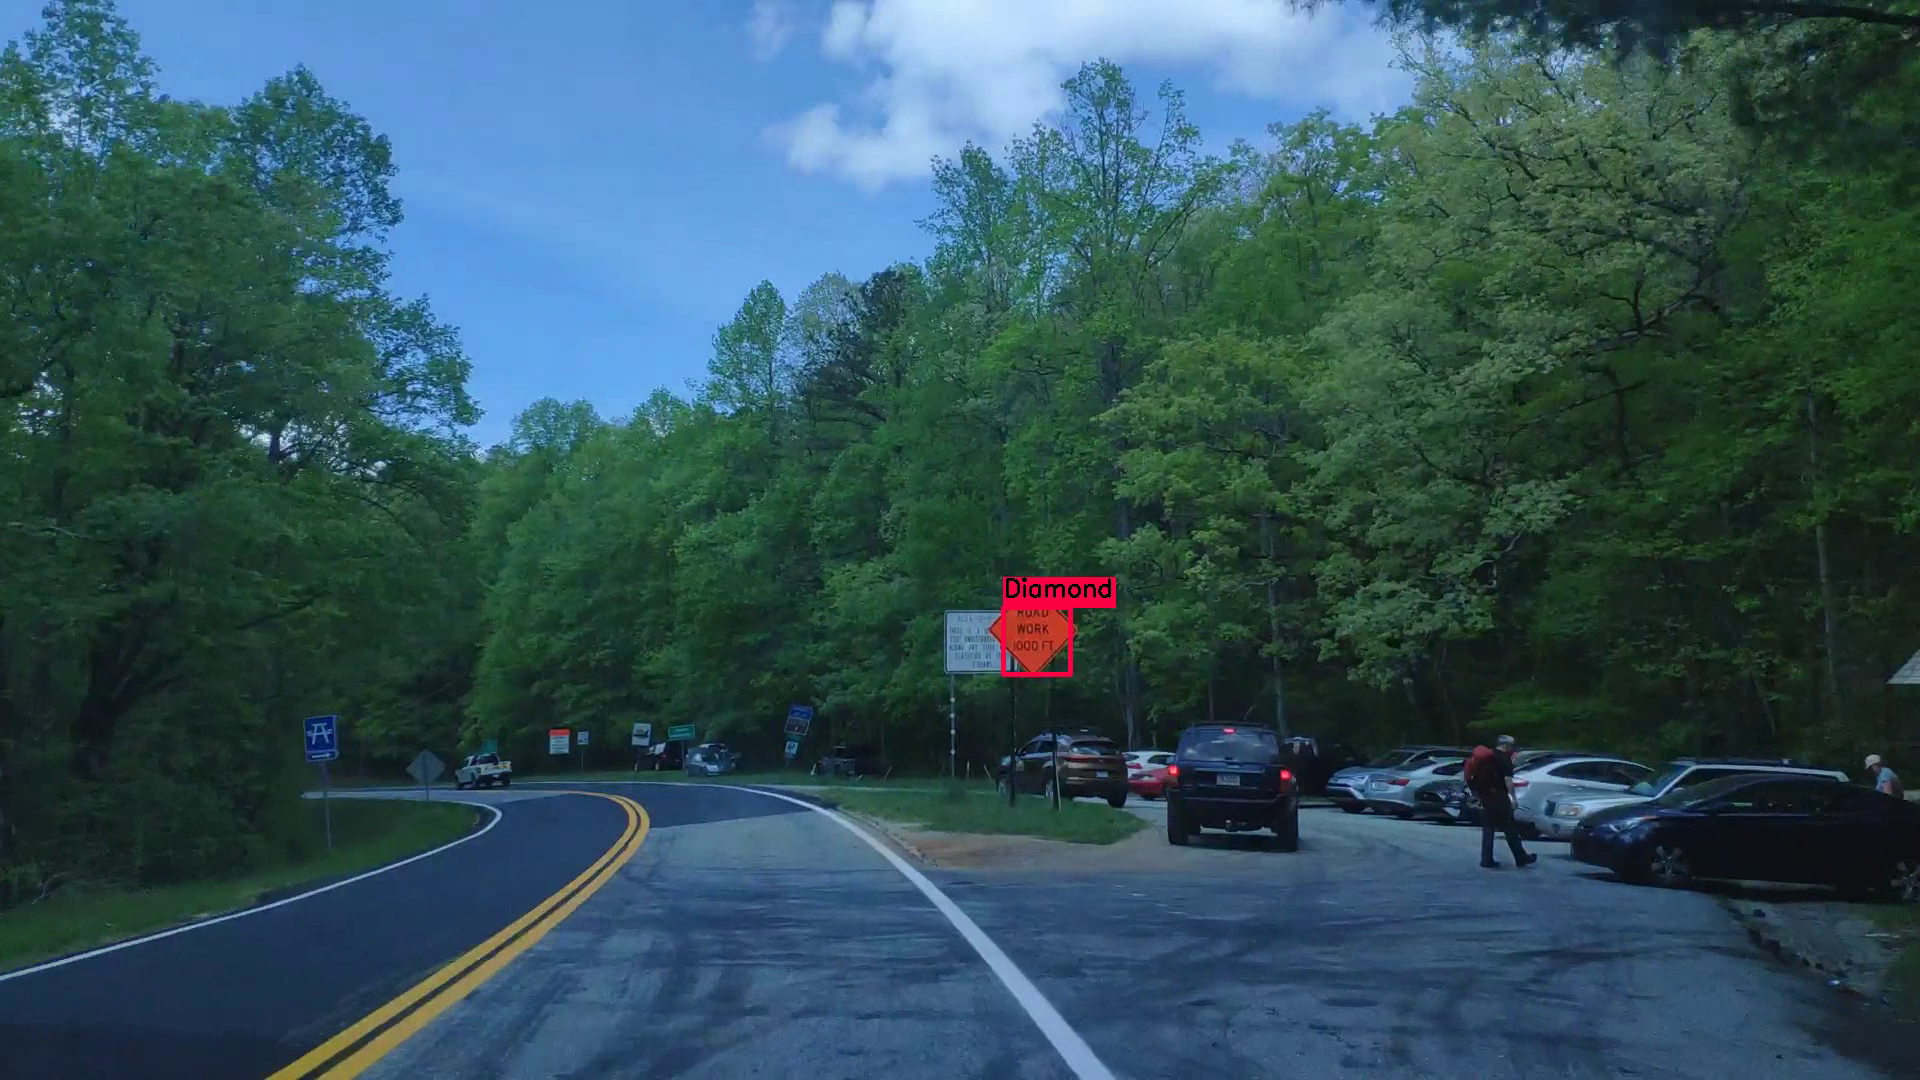
\includegraphics[width=0.99\linewidth]{figures/examples/sr2/FP/FP_07.png}
      \caption{Work zone diamond sign}
      \label{fig:workzoneFP}
    \end{subfigure}
    \begin{subfigure}[t]{.49\linewidth}
      \centering
      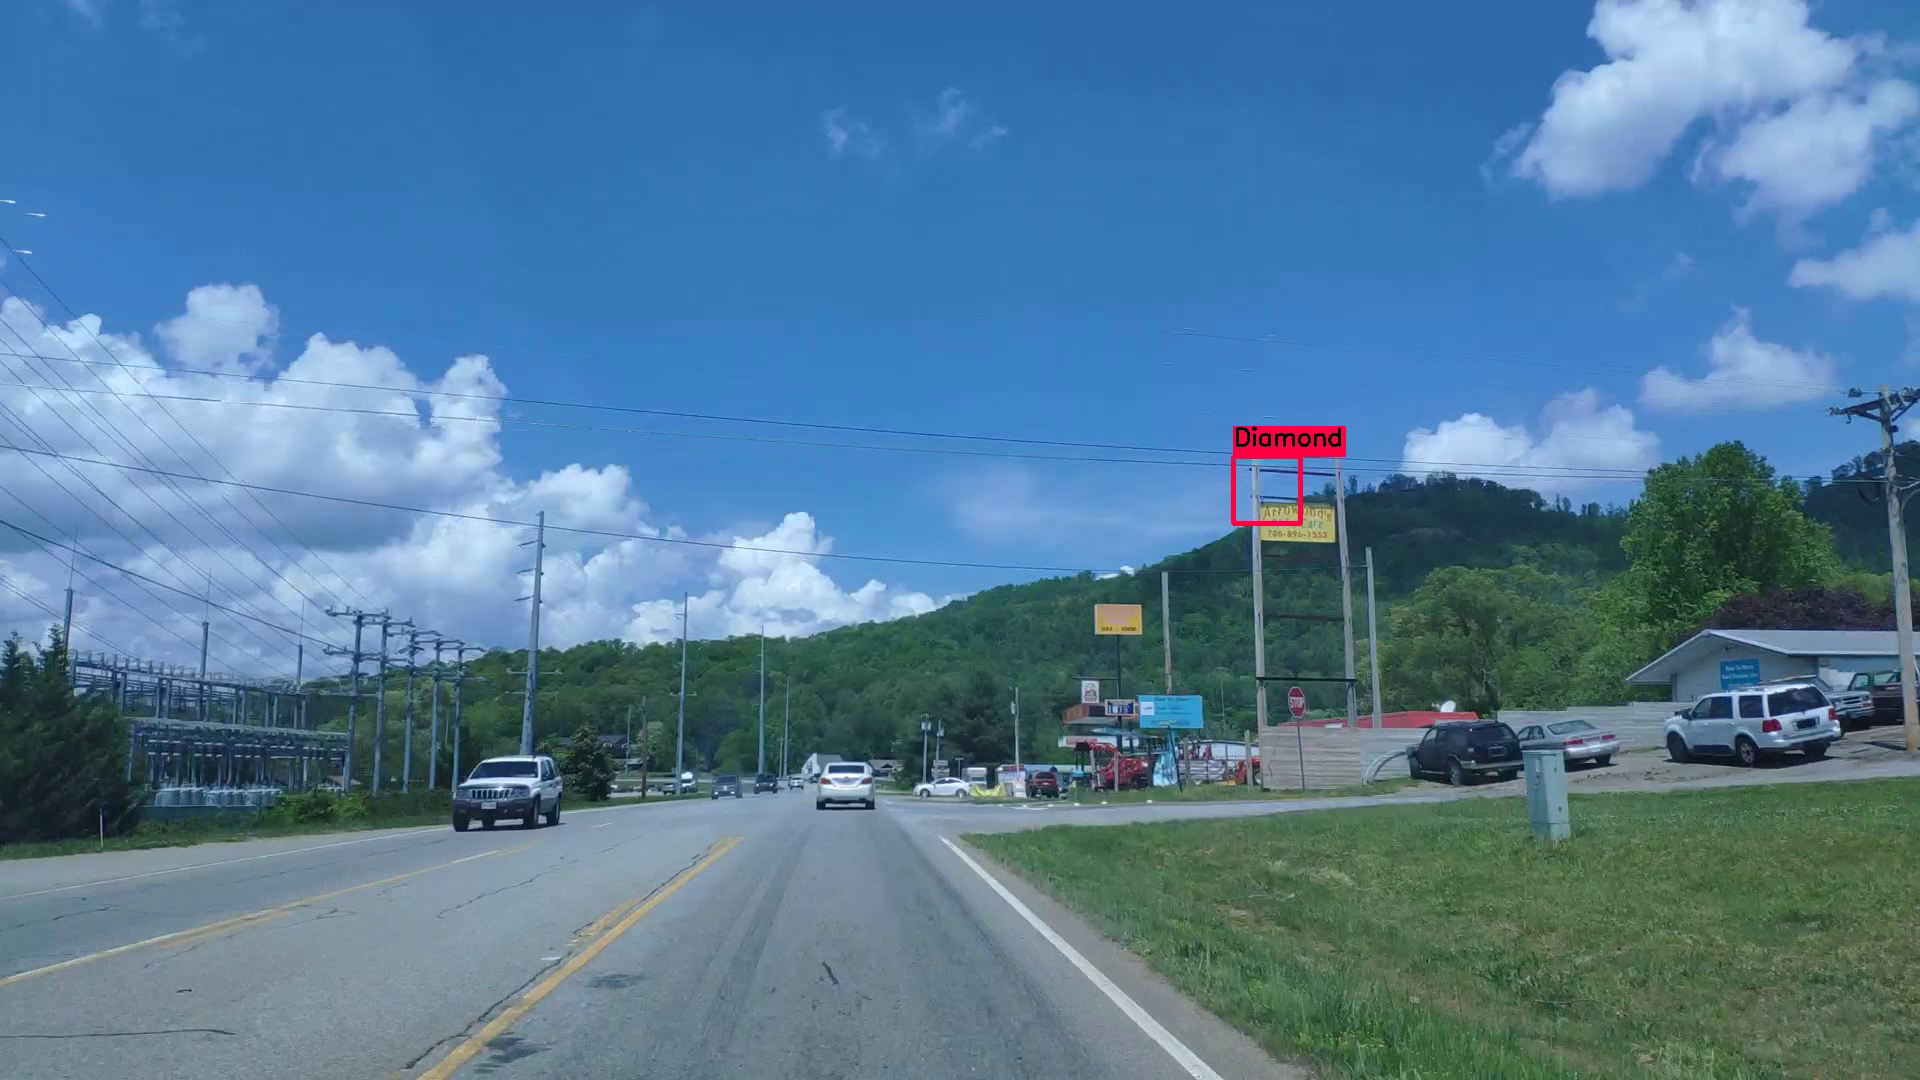
\includegraphics[width=0.99\linewidth]{figures/examples/sr2/FP/FP_17.png}
      \caption{Advertisement sign}
      \label{fig:advertisementFP}
    \end{subfigure}
    \caption{Example of False Positive case collected on State Road 2.}
    \label{fig:FPcases}
  \end{center}
\end{figure}

\paragraph{}
Our model as tendency to detect some yellow object as diamond traffic signs. In most of the cases, this false positive (FP) detection happen on other warning signs that are not supposed to be detected by this model and so were not part of the training data. This is the case illustrated by Figure \ref{fig:chevronFP}, this case is by far the most important case of FP, with more than twenty of them. However, this case is not really problematic because it is a sign, the best approach to fix this is to include it into the training as a new class. Another case of sign that are miss detected is the work zone sign, as illustrated by figure \ref{fig:workzoneFP}, we encountered six different signs like that in our testing, here the best solution to counter that is to wait a classification step to correct it. It is important to notice that most of the work zone signs are not detected as expected.

Another category of false positive we observed, is the yellow signalization. A first example is the signalization at the beginning of a guard rail. This case is illustrated on Figure \ref{fig:guardRailFP}, we observed three such case on the entire run. The second one is the signalization on the back of the Georgia DOT truck we were following the whole time. We get two FP out of this warning bend as illustrated on Figure \ref{fig:GDOTtruckFP}.

The remaining FP were yellow object present around the road. This kind of objects include, a car light from Figure \ref{fig:carLightFP}, a part of a yellow digger, on Figure \ref{fig:diggerFP}, yellow advertisement signs as in Figure \ref{fig:advertisementFP} or plants like displayed on Figure \ref{fig:plantFP}. Of all those case, only the last two appeared three times while the other only once on all the frames, and they all appear only in one frame, making them easy to filter out.

All this example show more a weakness of the dataset we use for training than a real failure our architecture, although, the final number of false positive we get were is still small regarding the number of true positive.

\subsubsection{False Negative cases}

\begin{figure}
  \begin{center}
    \begin{subfigure}[t]{.49\linewidth}
      \centering
      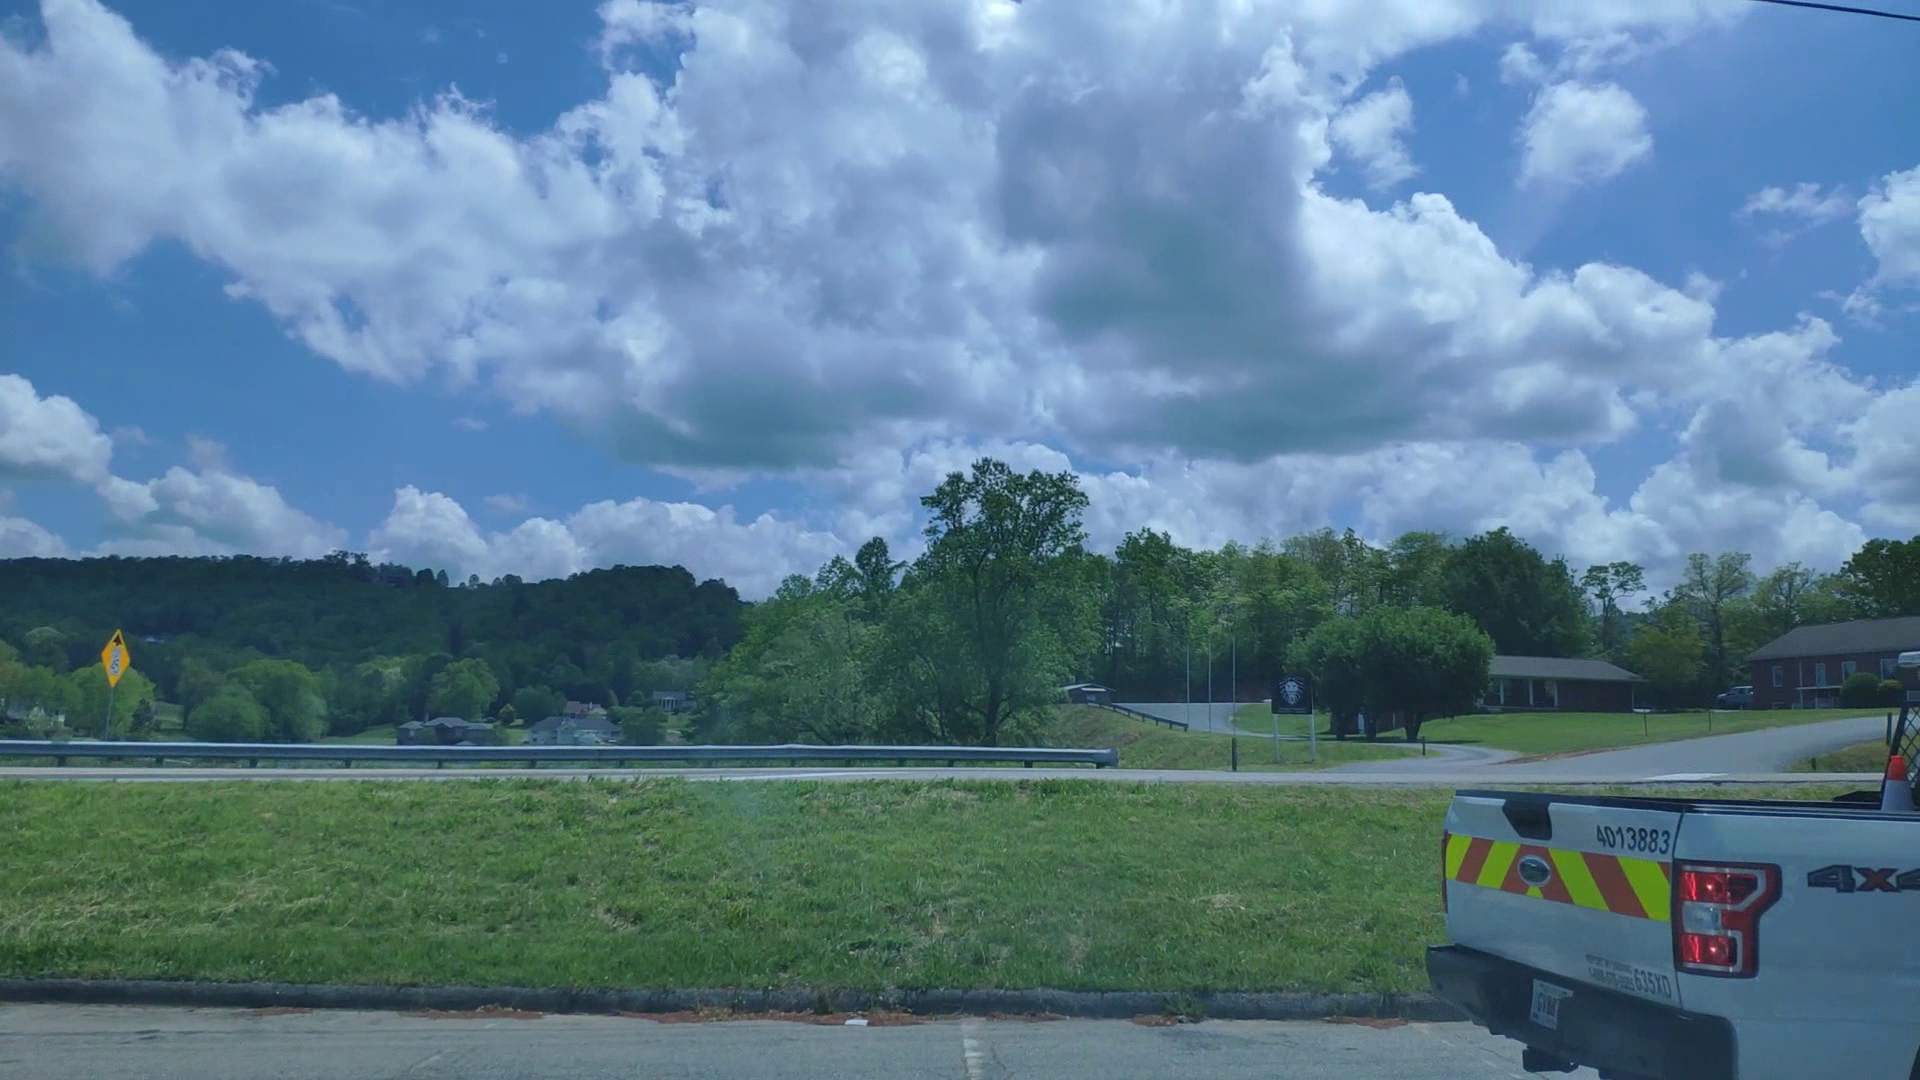
\includegraphics[width=0.99\linewidth]{figures/examples/sr2/FN/FN_01.png}
      \caption{Perspective transformation}
      \label{fig:perspecFN}
    \end{subfigure}
    \begin{subfigure}[t]{.49\linewidth}
      \centering
      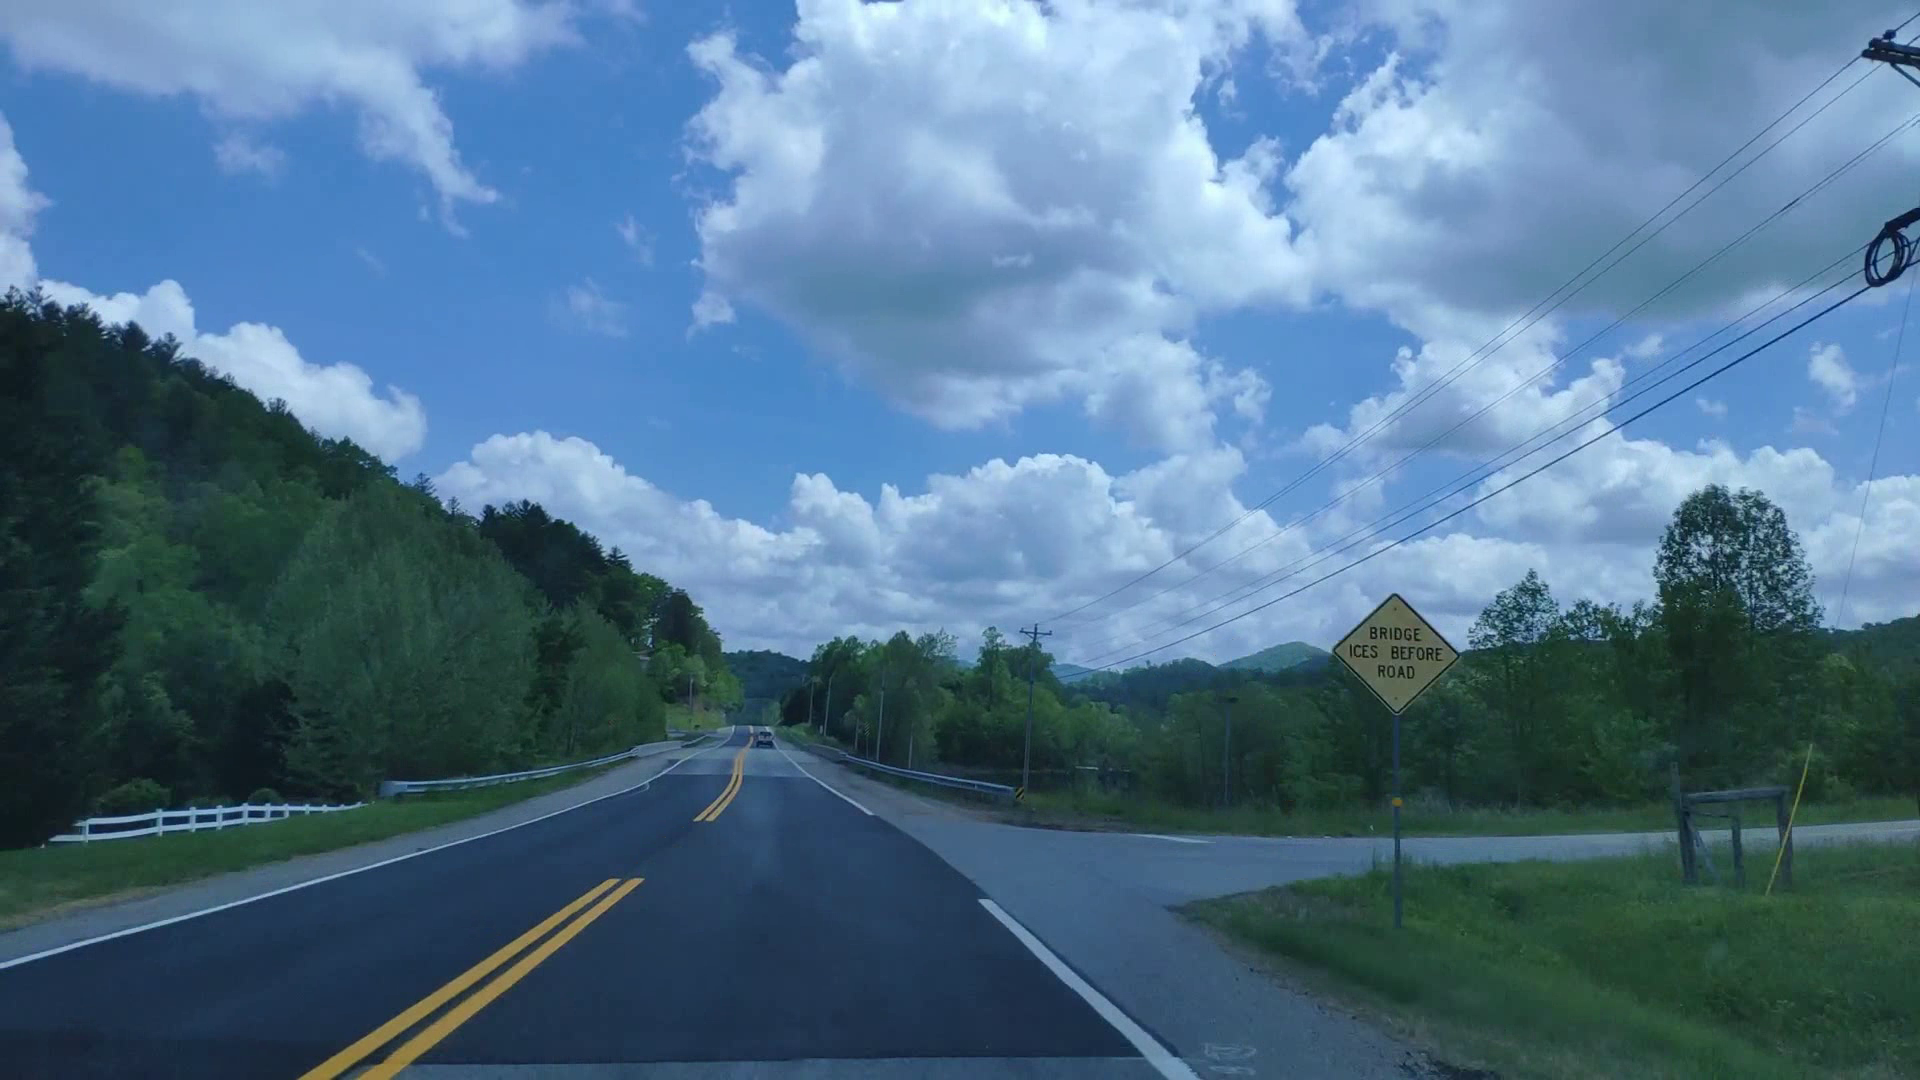
\includegraphics[width=0.99\linewidth]{figures/examples/sr2/FN/FN_02.png}
      \caption{Light, faded sign}
    \end{subfigure}
    \begin{subfigure}[t]{.49\linewidth}
      \centering
      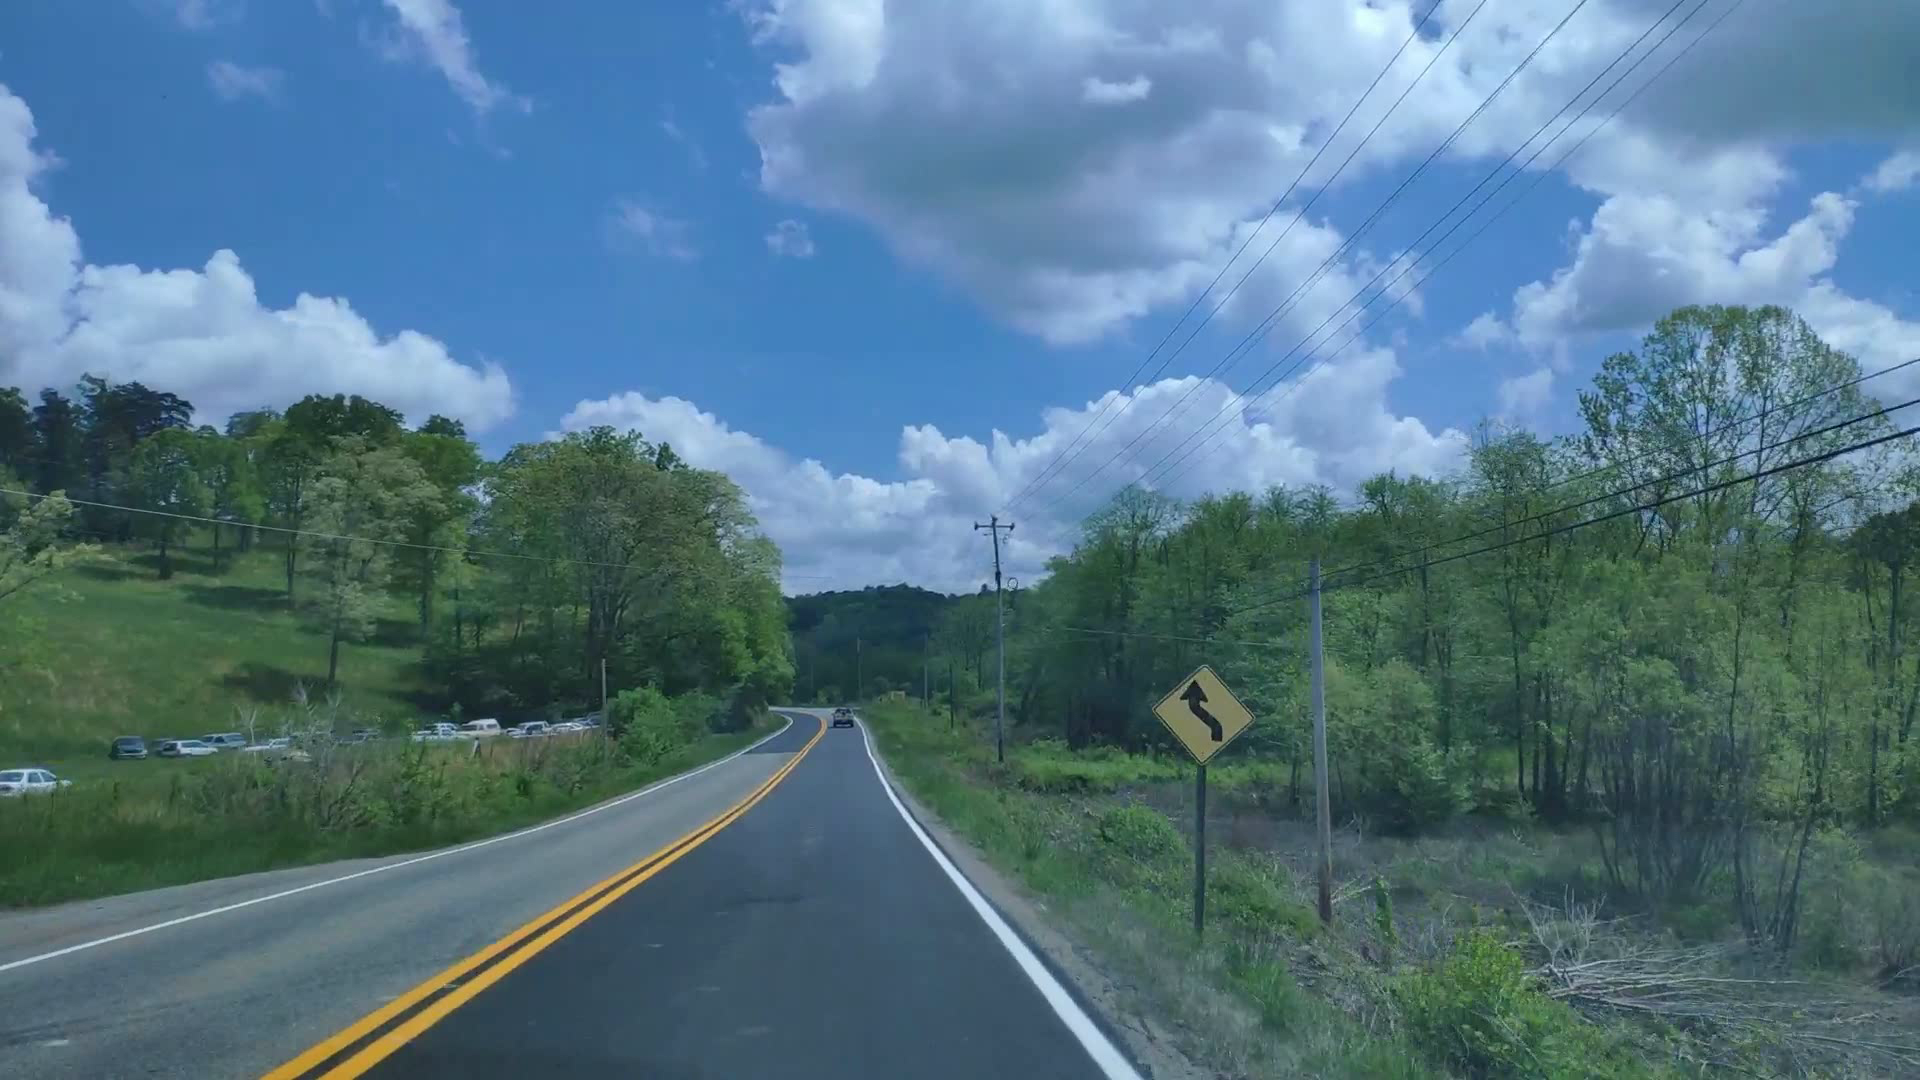
\includegraphics[width=0.99\linewidth]{figures/examples/sr2/FN/FN_03.png}
      \caption{Light, faded sign}
    \end{subfigure}
    \begin{subfigure}[t]{.49\linewidth}
      \centering
      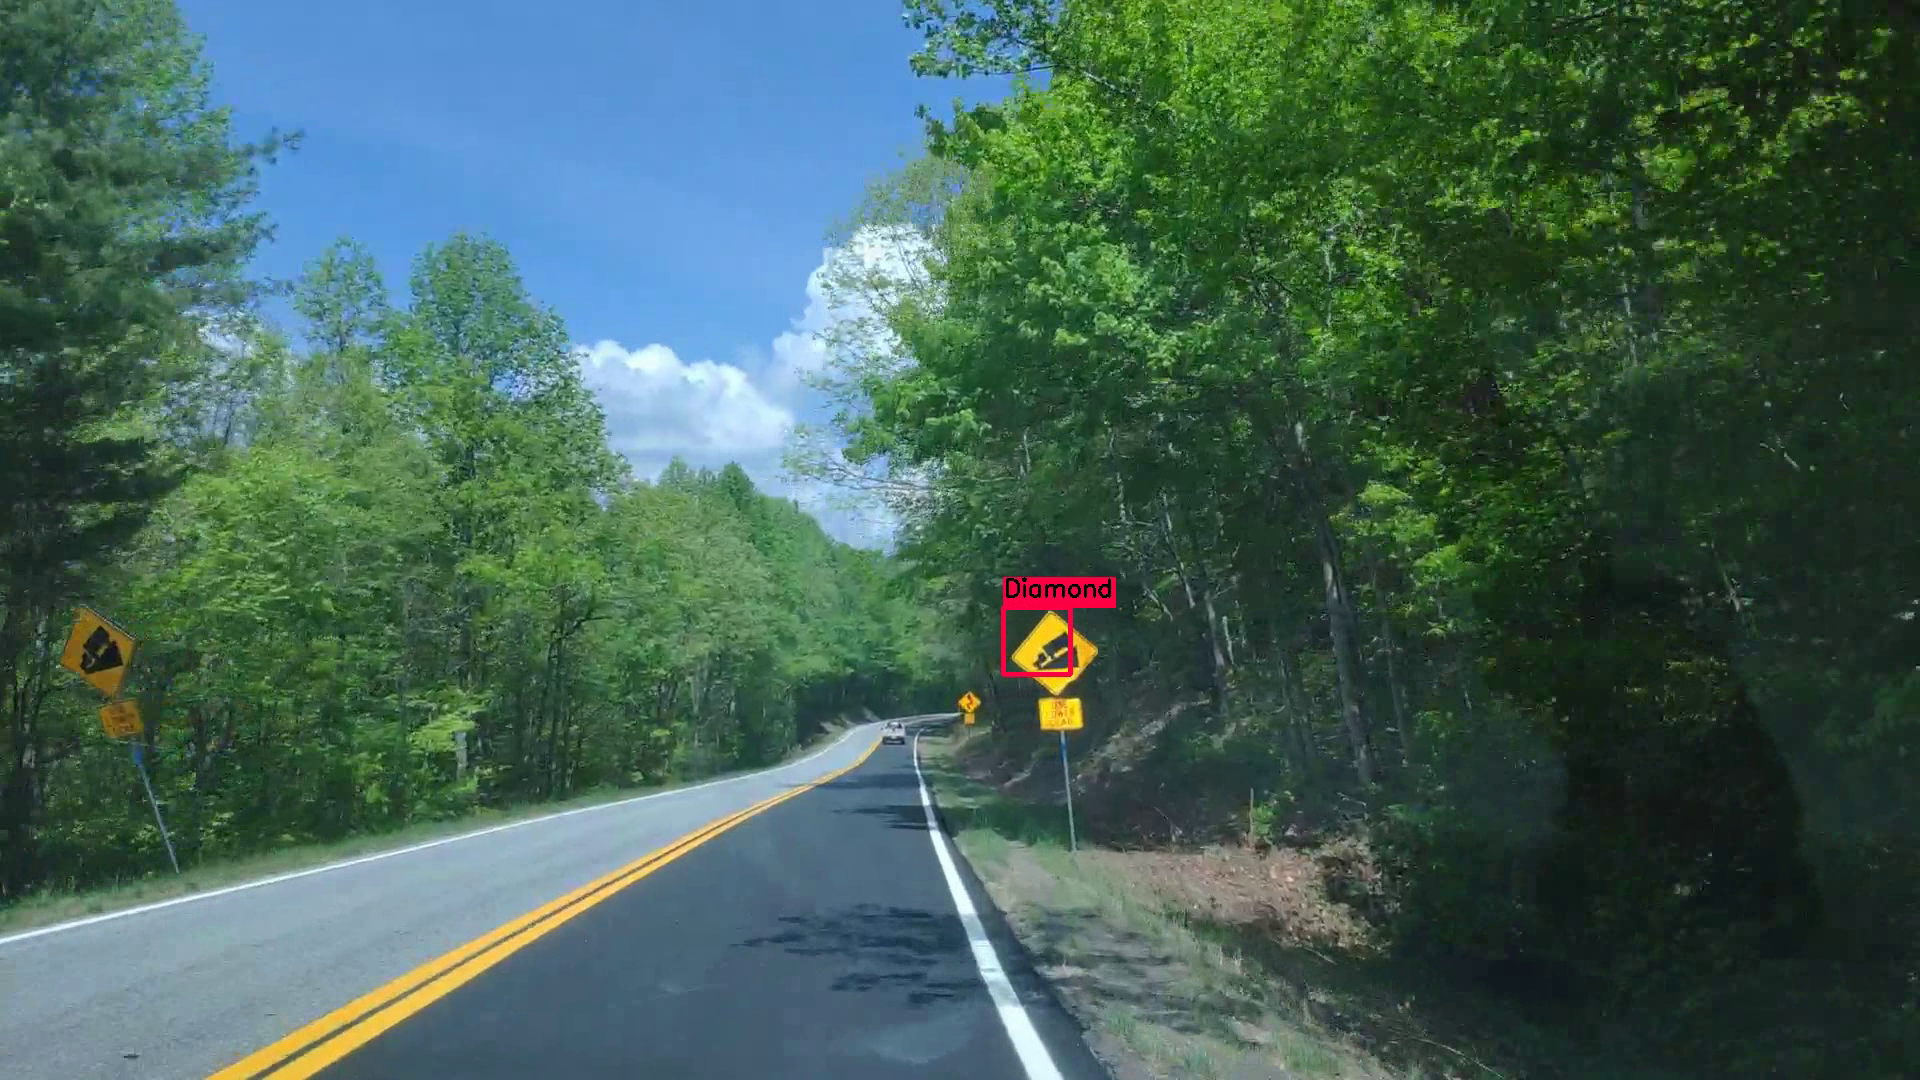
\includegraphics[width=0.99\linewidth]{figures/examples/sr2/FN/FN_09.png}
      \caption{Sign on the other side of the road}
      \label{fig:othersideFN}
    \end{subfigure}
    \begin{subfigure}[t]{.49\linewidth}
      \centering
      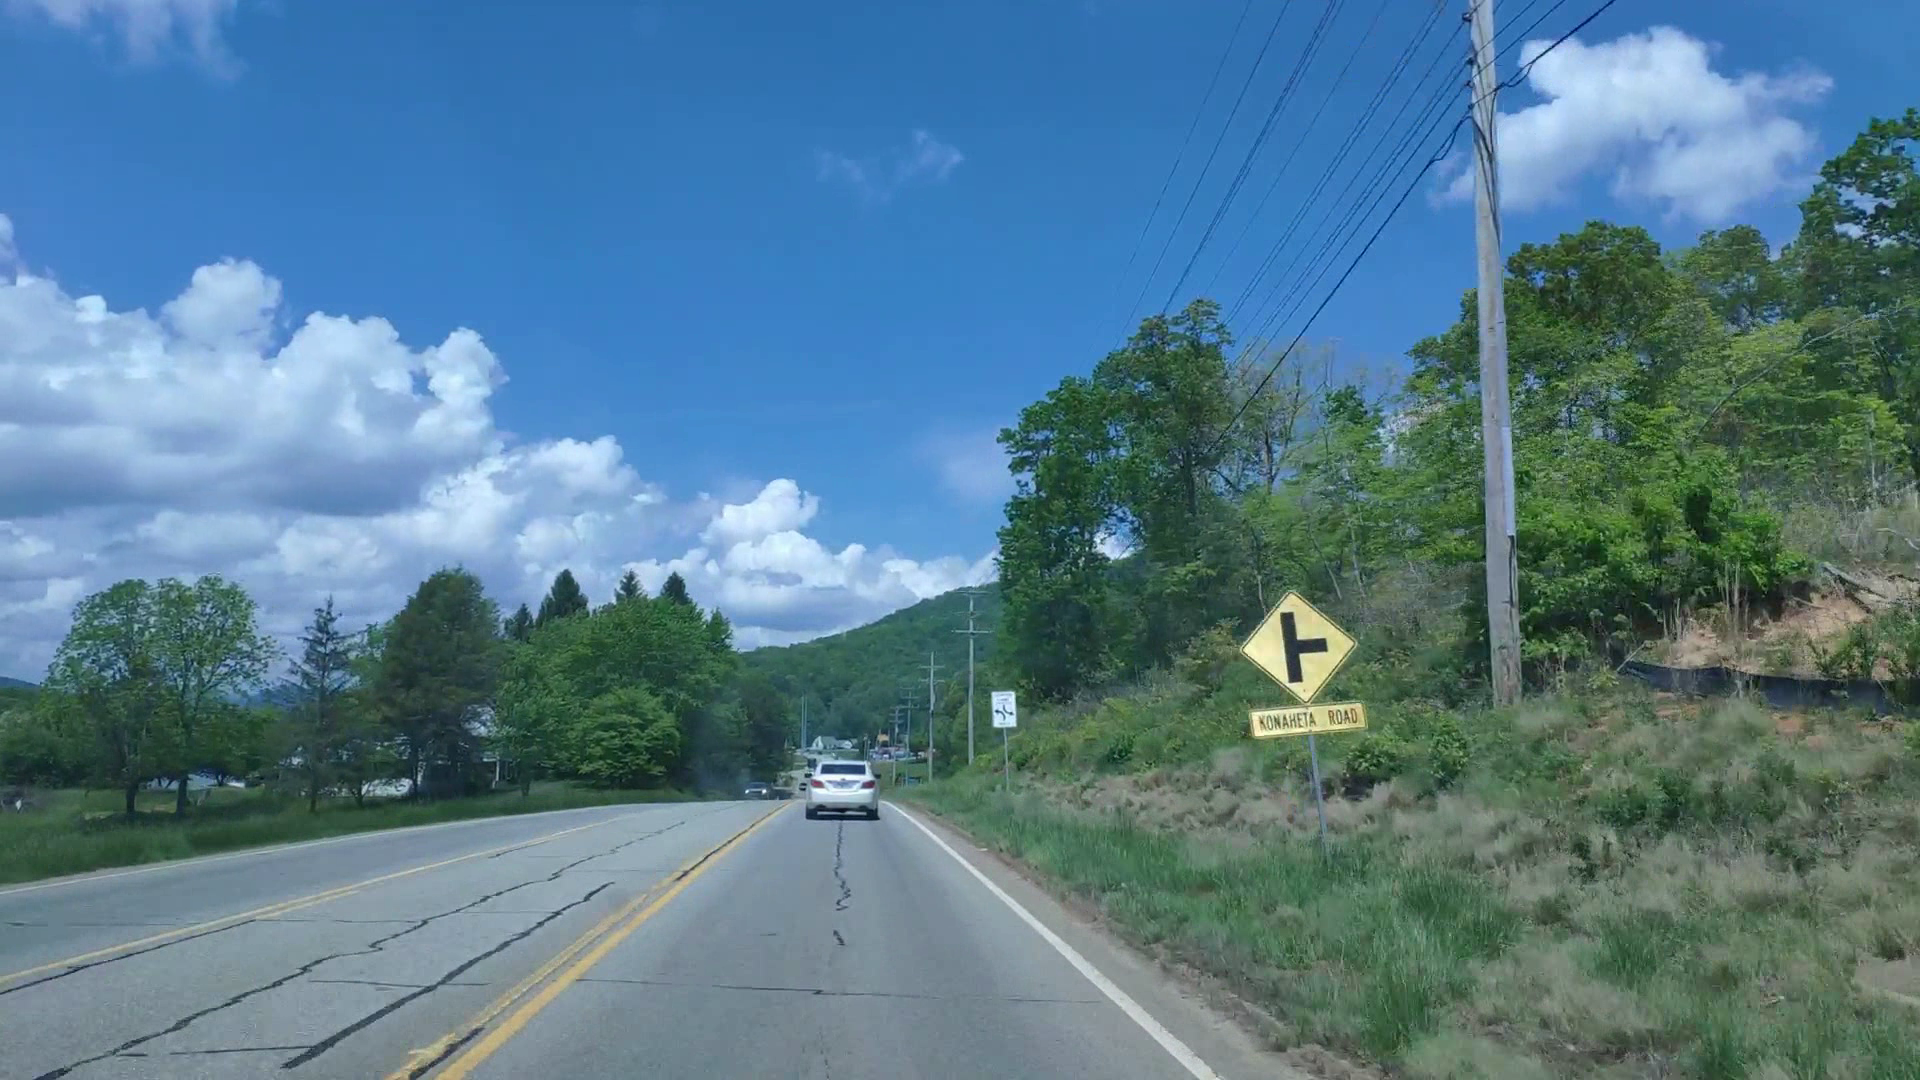
\includegraphics[width=0.99\linewidth]{figures/examples/sr2/FN/FN_10.png}
      \caption{Light, faded sign}
    \end{subfigure}
    \begin{subfigure}[t]{.49\linewidth}
      \centering
      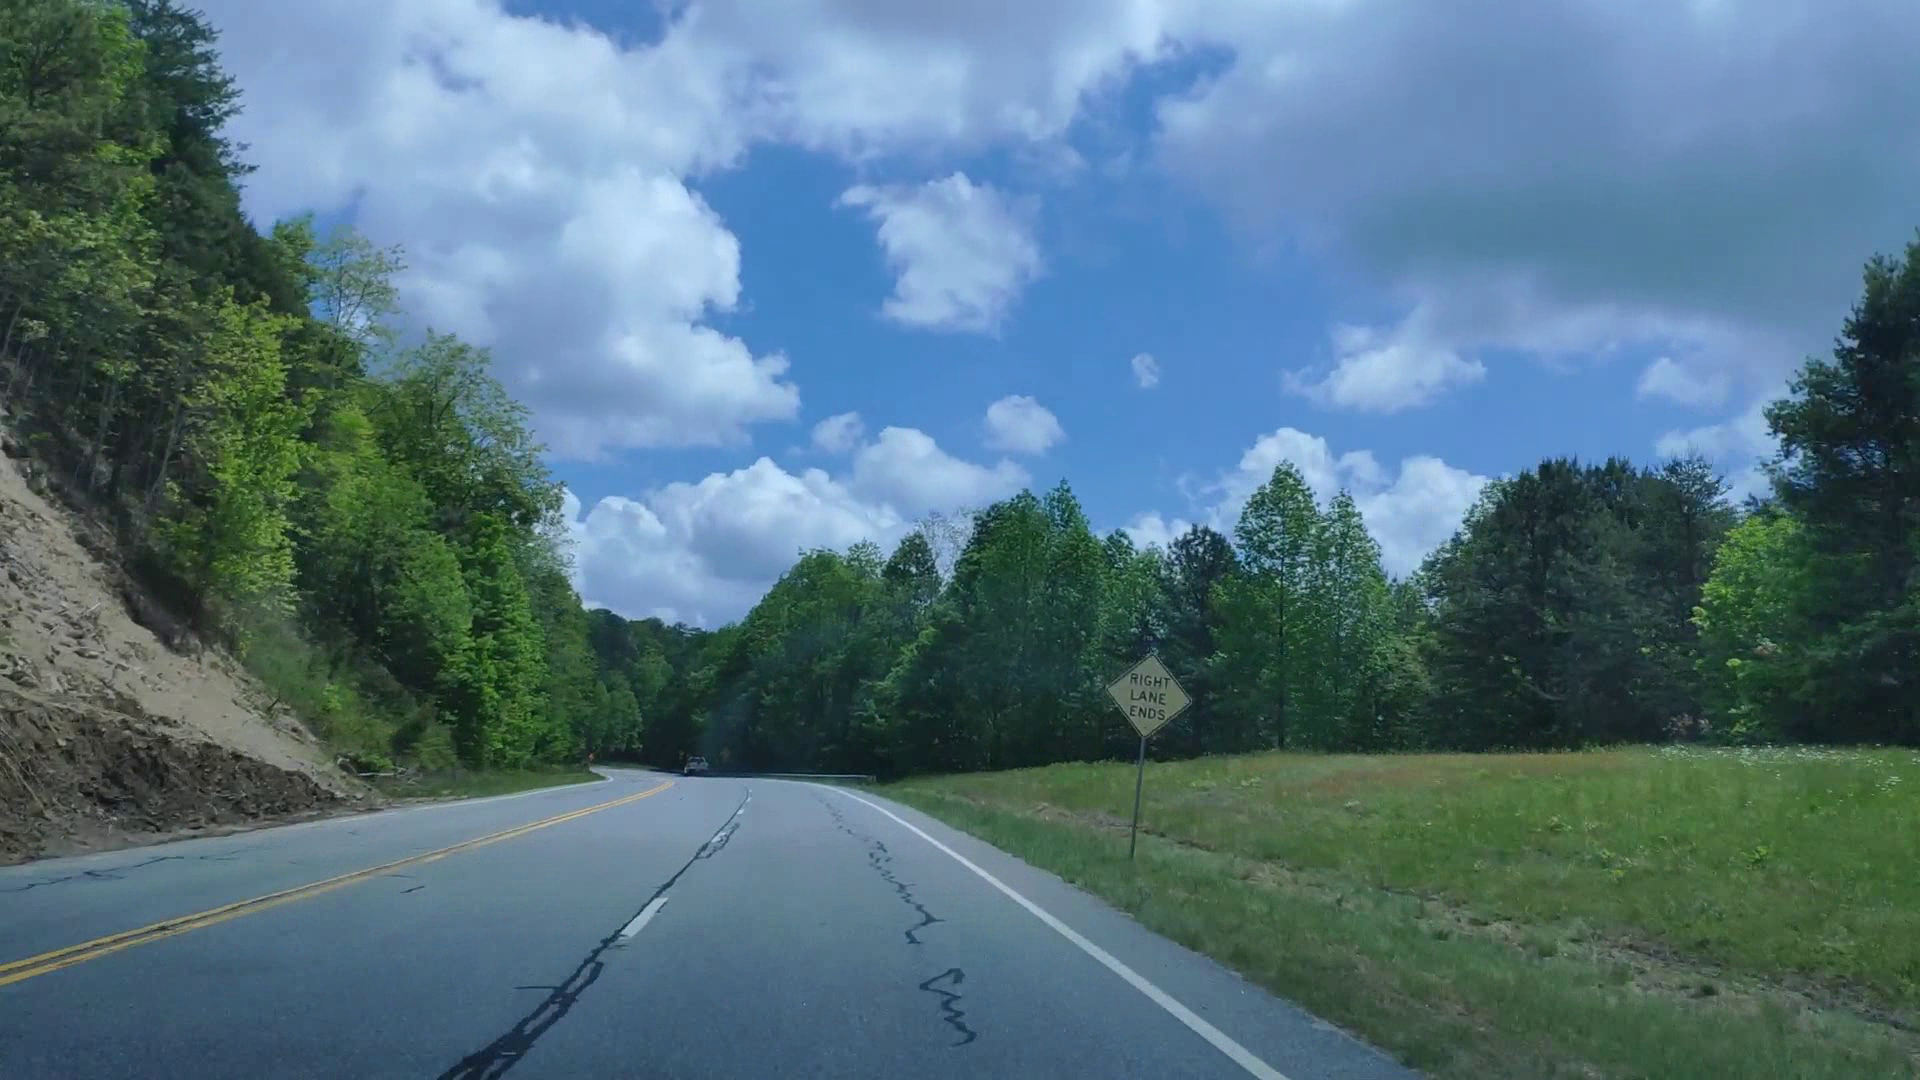
\includegraphics[width=0.99\linewidth]{figures/examples/sr2/FN/FN_06.png}
      \caption{Light, faded sign}
    \end{subfigure}
    \begin{subfigure}[t]{.49\linewidth}
      \centering
      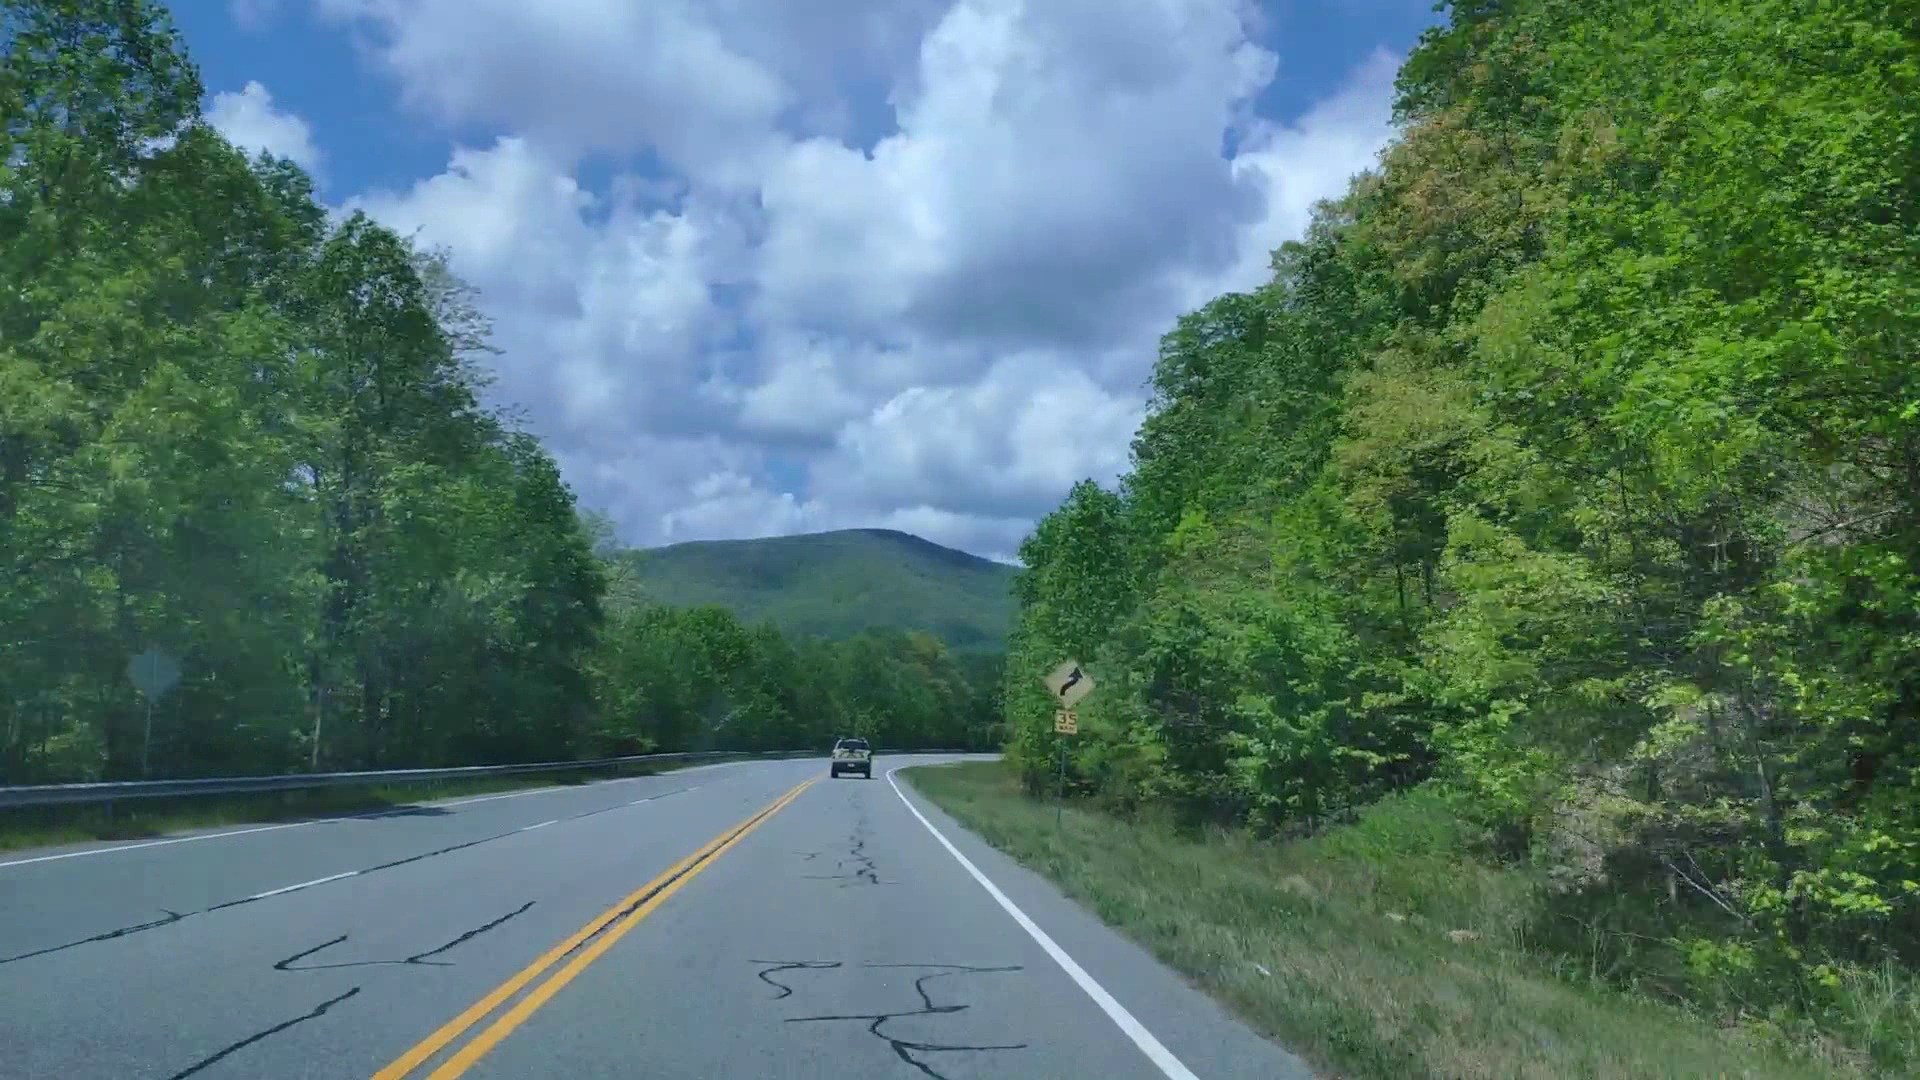
\includegraphics[width=0.99\linewidth]{figures/examples/sr2/FN/FN_07.png}
      \caption{Light, faded sign}
    \end{subfigure}
    \begin{subfigure}[t]{.49\linewidth}
      \centering
      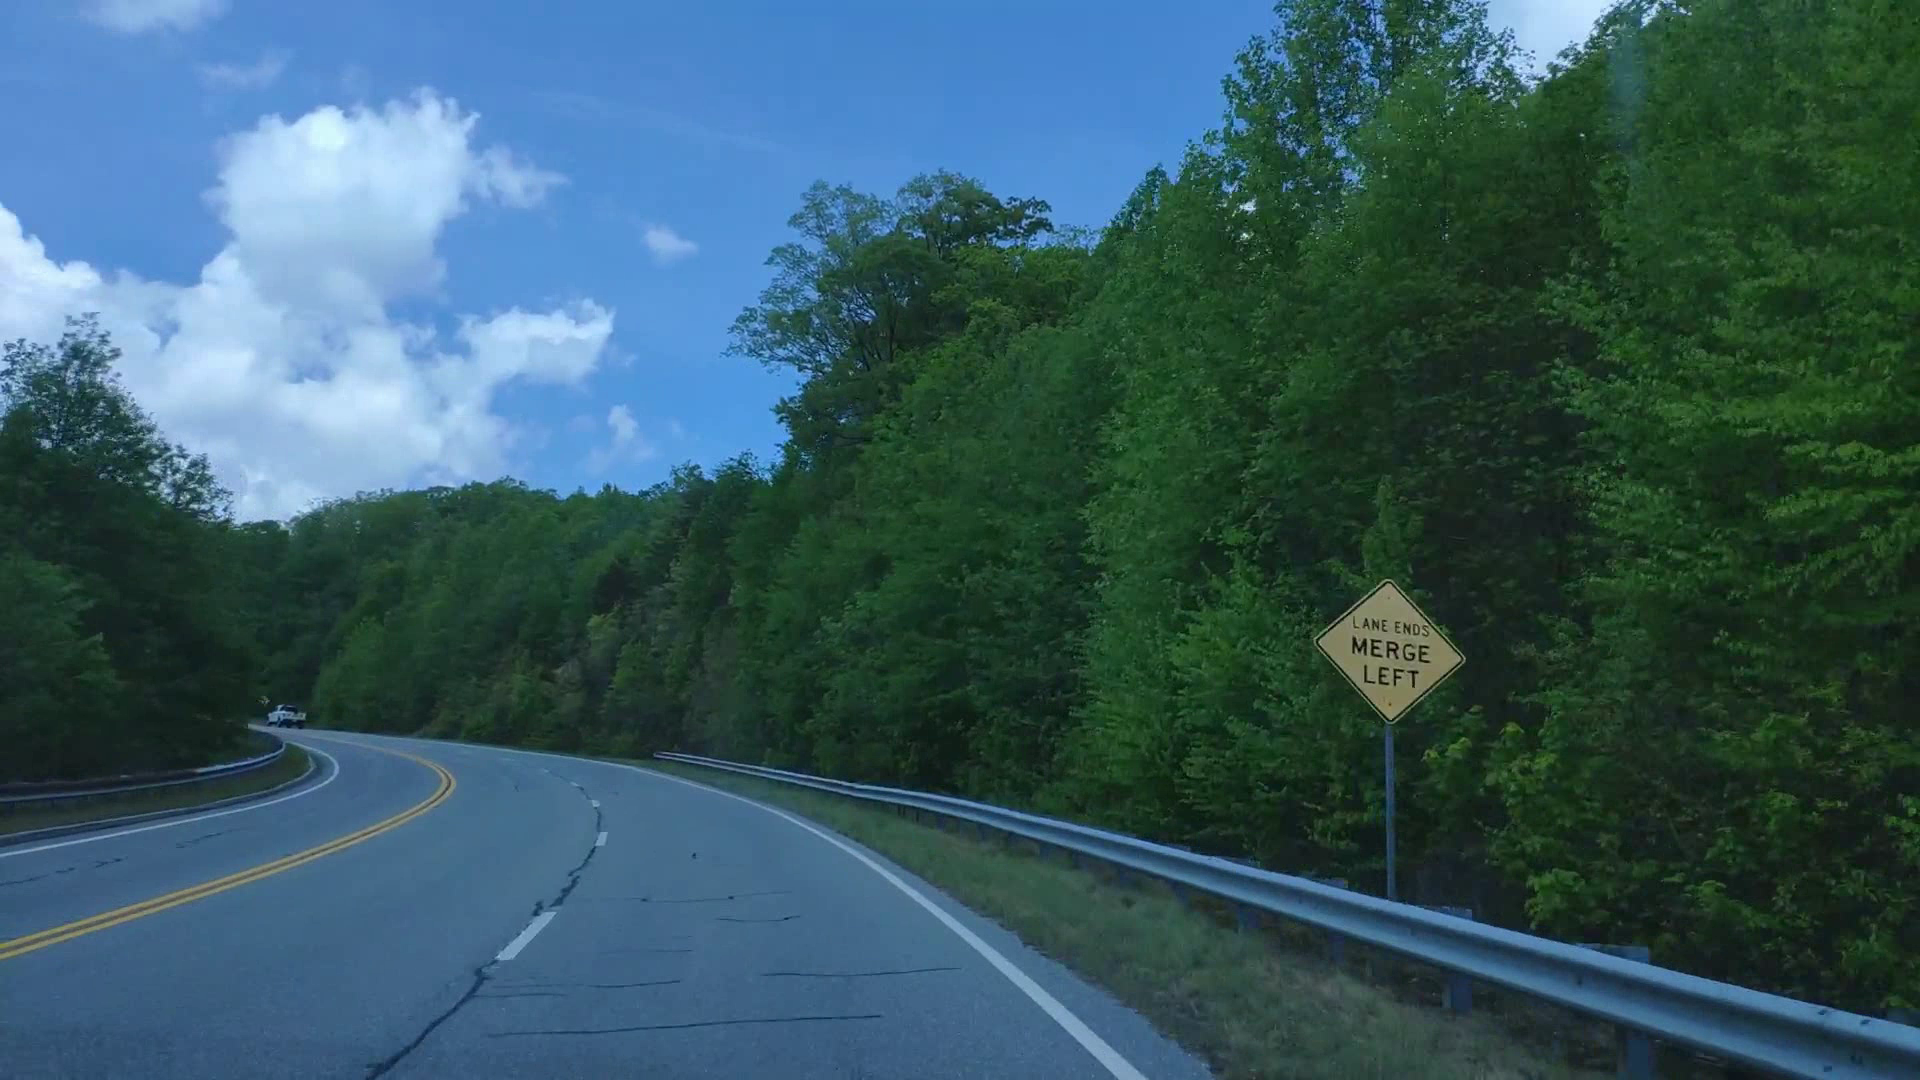
\includegraphics[width=0.99\linewidth]{figures/examples/sr2/FN/FN_08.png}
      \caption{Light, faded sign}
    \end{subfigure}
    \caption{Example of False Negative cases collected on State Road 2.}
    \label{fig:FNcases}
  \end{center}
\end{figure}

\paragraph{}
In total, we counted 10 FN on this set of frames. One in Figure \ref{fig:perspecFN}, is due to a large perspective transformation and a small size. We can note that this sign is latter detected when driving on the road. Another case, representing two false positive, is sign on the left side of the road, one of these cases is illustrated by Figure \ref{fig:othersideFN}, such cases are more difficult to detect because of the orientation of the camera and in both of these cases poor lighting condition and sign condition. However, the most common case is light, faded sign that are not properly detected, as you can see on Figure \ref{fig:FNcases}. This number of similar case, let us believe that it is a result of the lack of diversity in our training data. One way to fix that would be to set up a more aggressive data augmentation on the color point of view. More experiments are needed to rule about the responsibility of the model.

\subsubsection{Interesting True positive cases}

\begin{figure}
  \begin{center}
    \begin{subfigure}[t]{.49\linewidth}
      \centering
      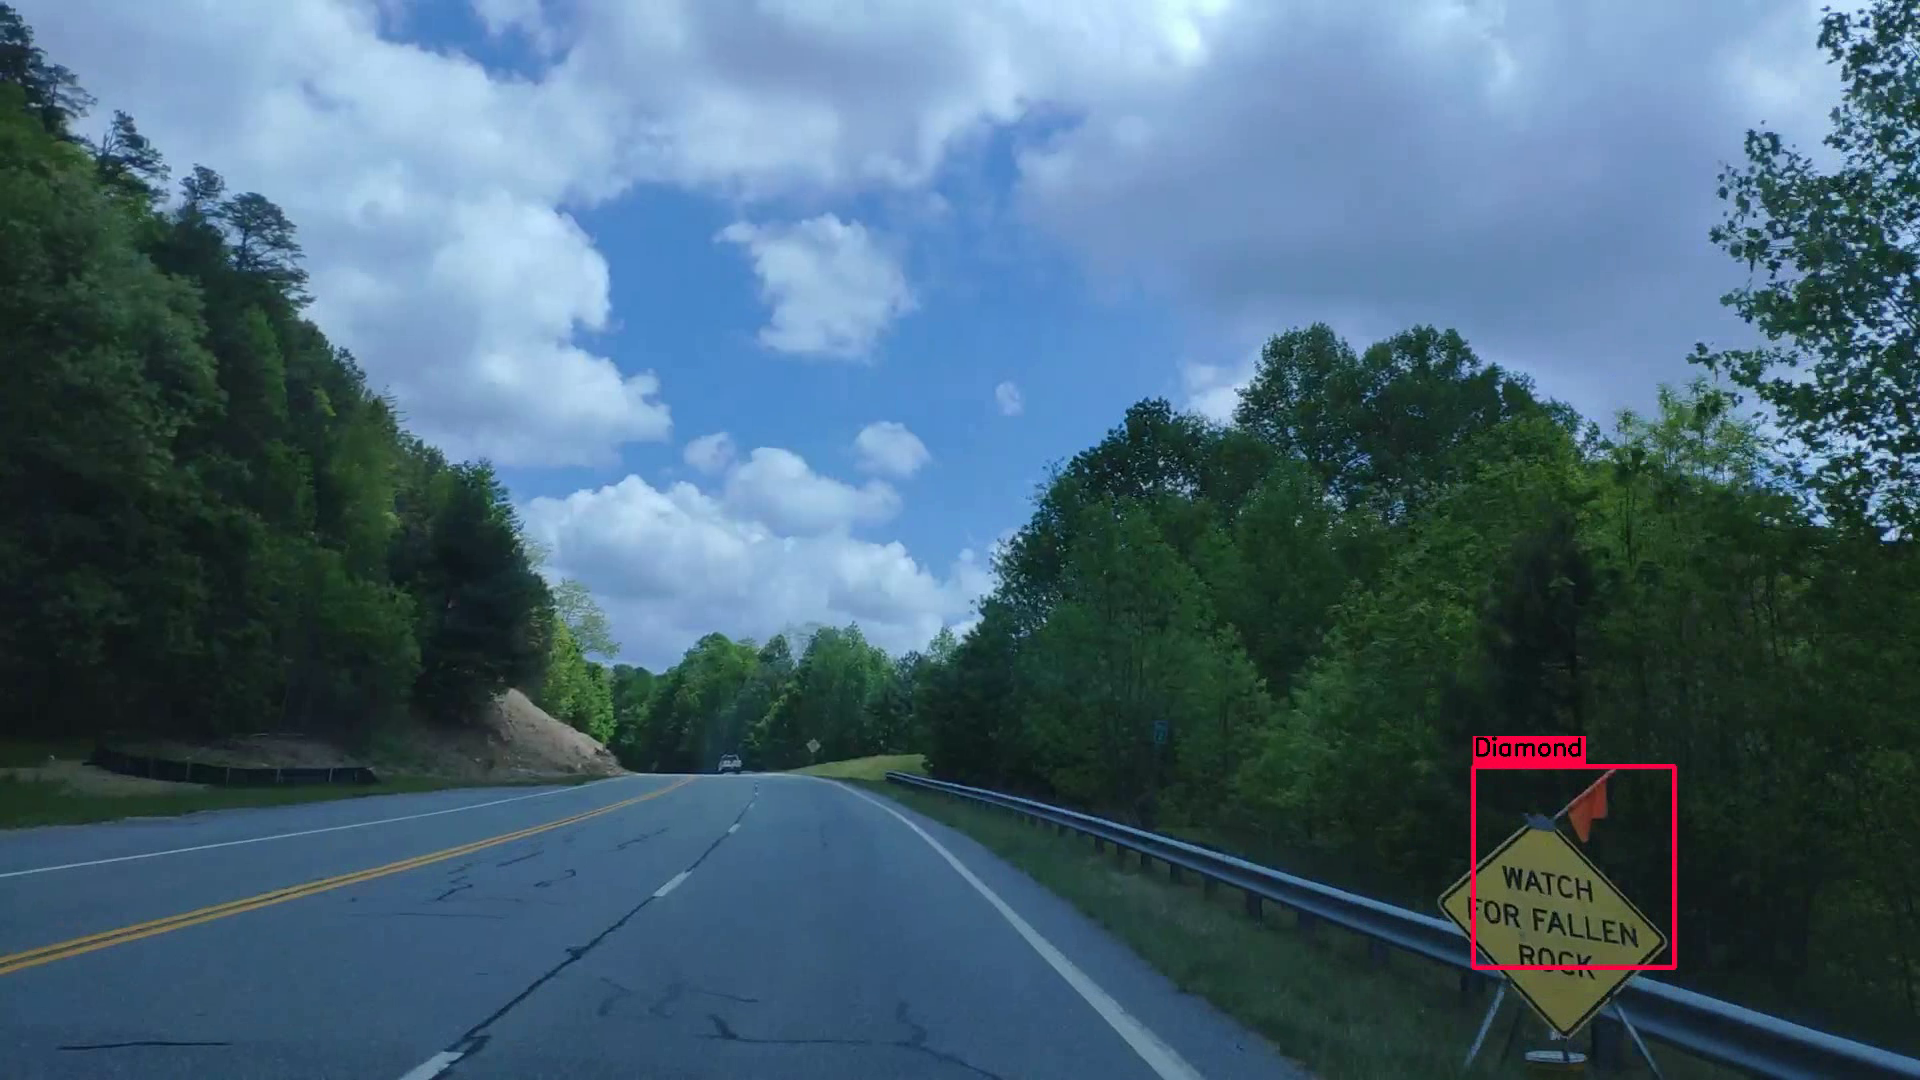
\includegraphics[width=0.99\linewidth]{figures/examples/sr2/TP/TP_01.png}
      \caption{Temporary sign}
      \label{fig:temporaryTP}
    \end{subfigure}
    \begin{subfigure}[t]{.49\linewidth}
      \centering
      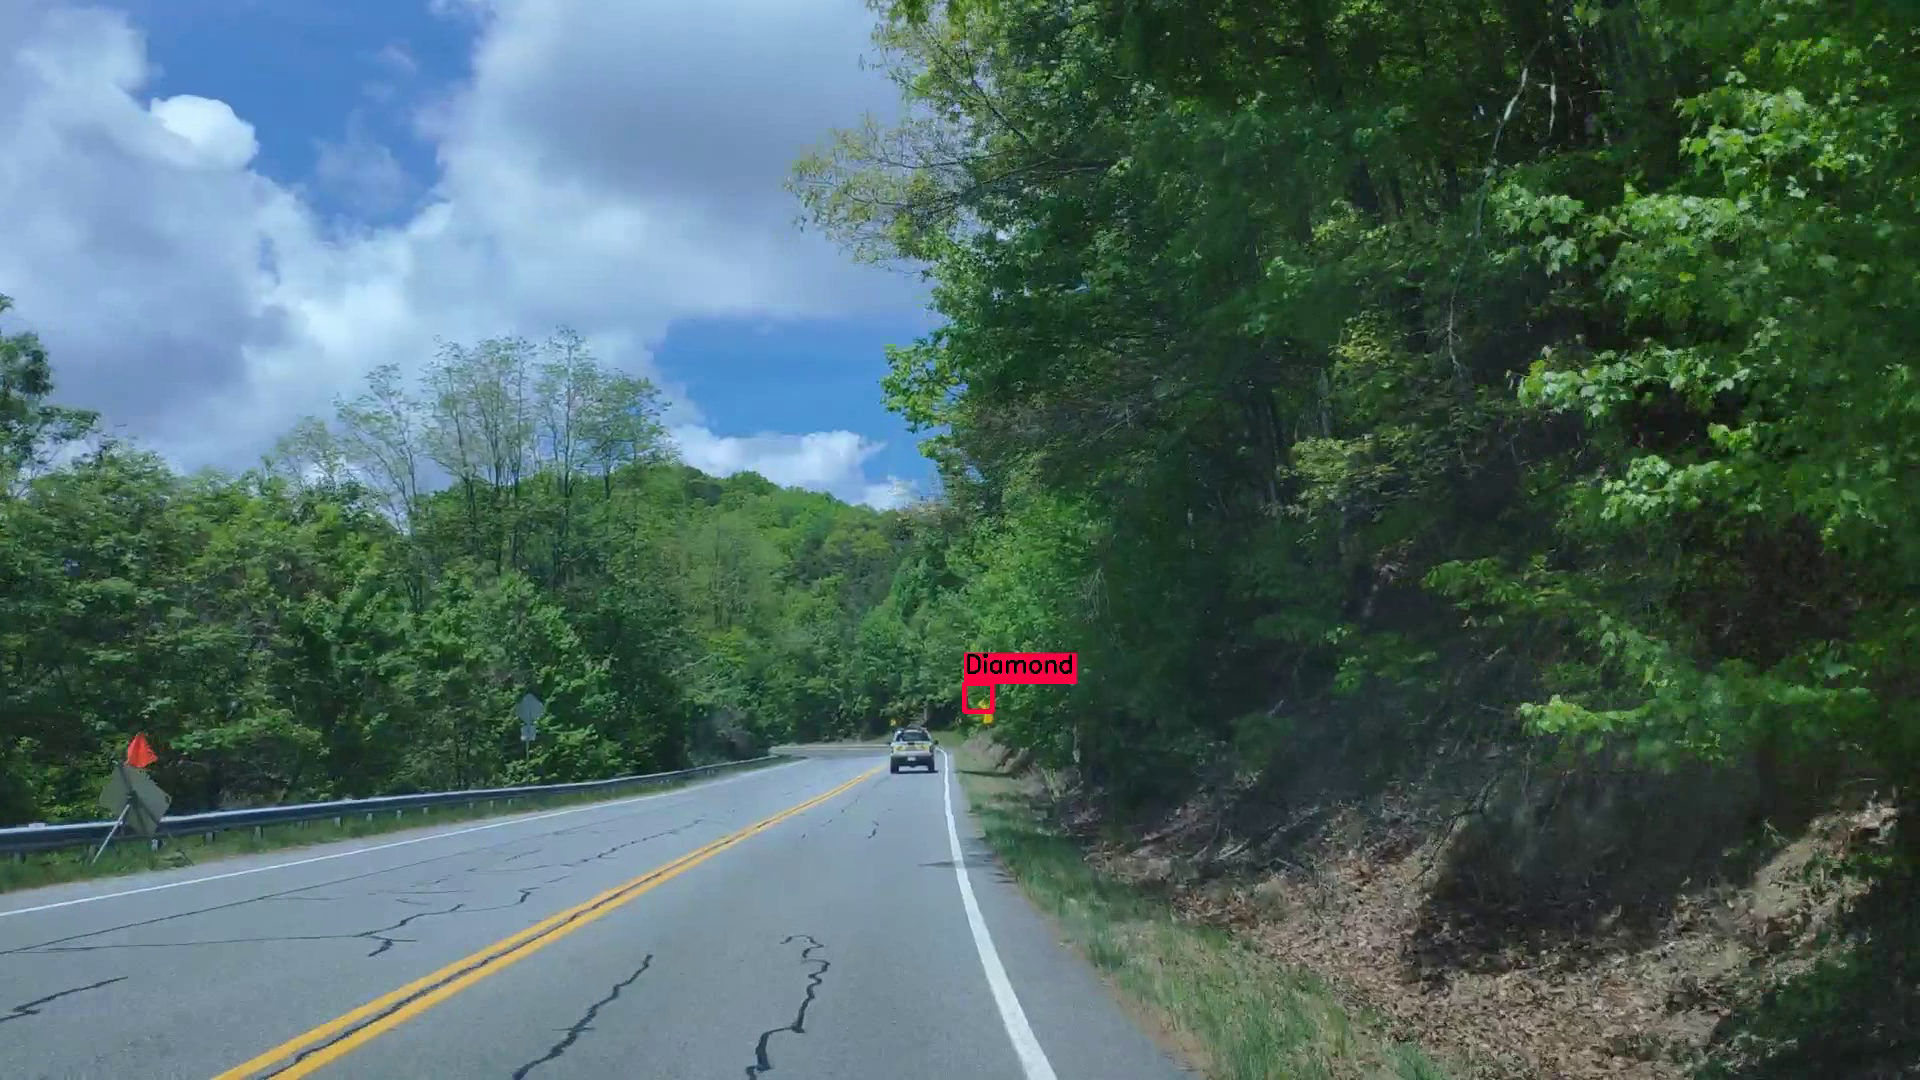
\includegraphics[width=0.99\linewidth]{figures/examples/sr2/TP/TP_09.png}
      \caption{Small and partially obstructed sign}
      \label{fig:farobstTP}
    \end{subfigure}
    \begin{subfigure}[t]{.49\linewidth}
      \centering
      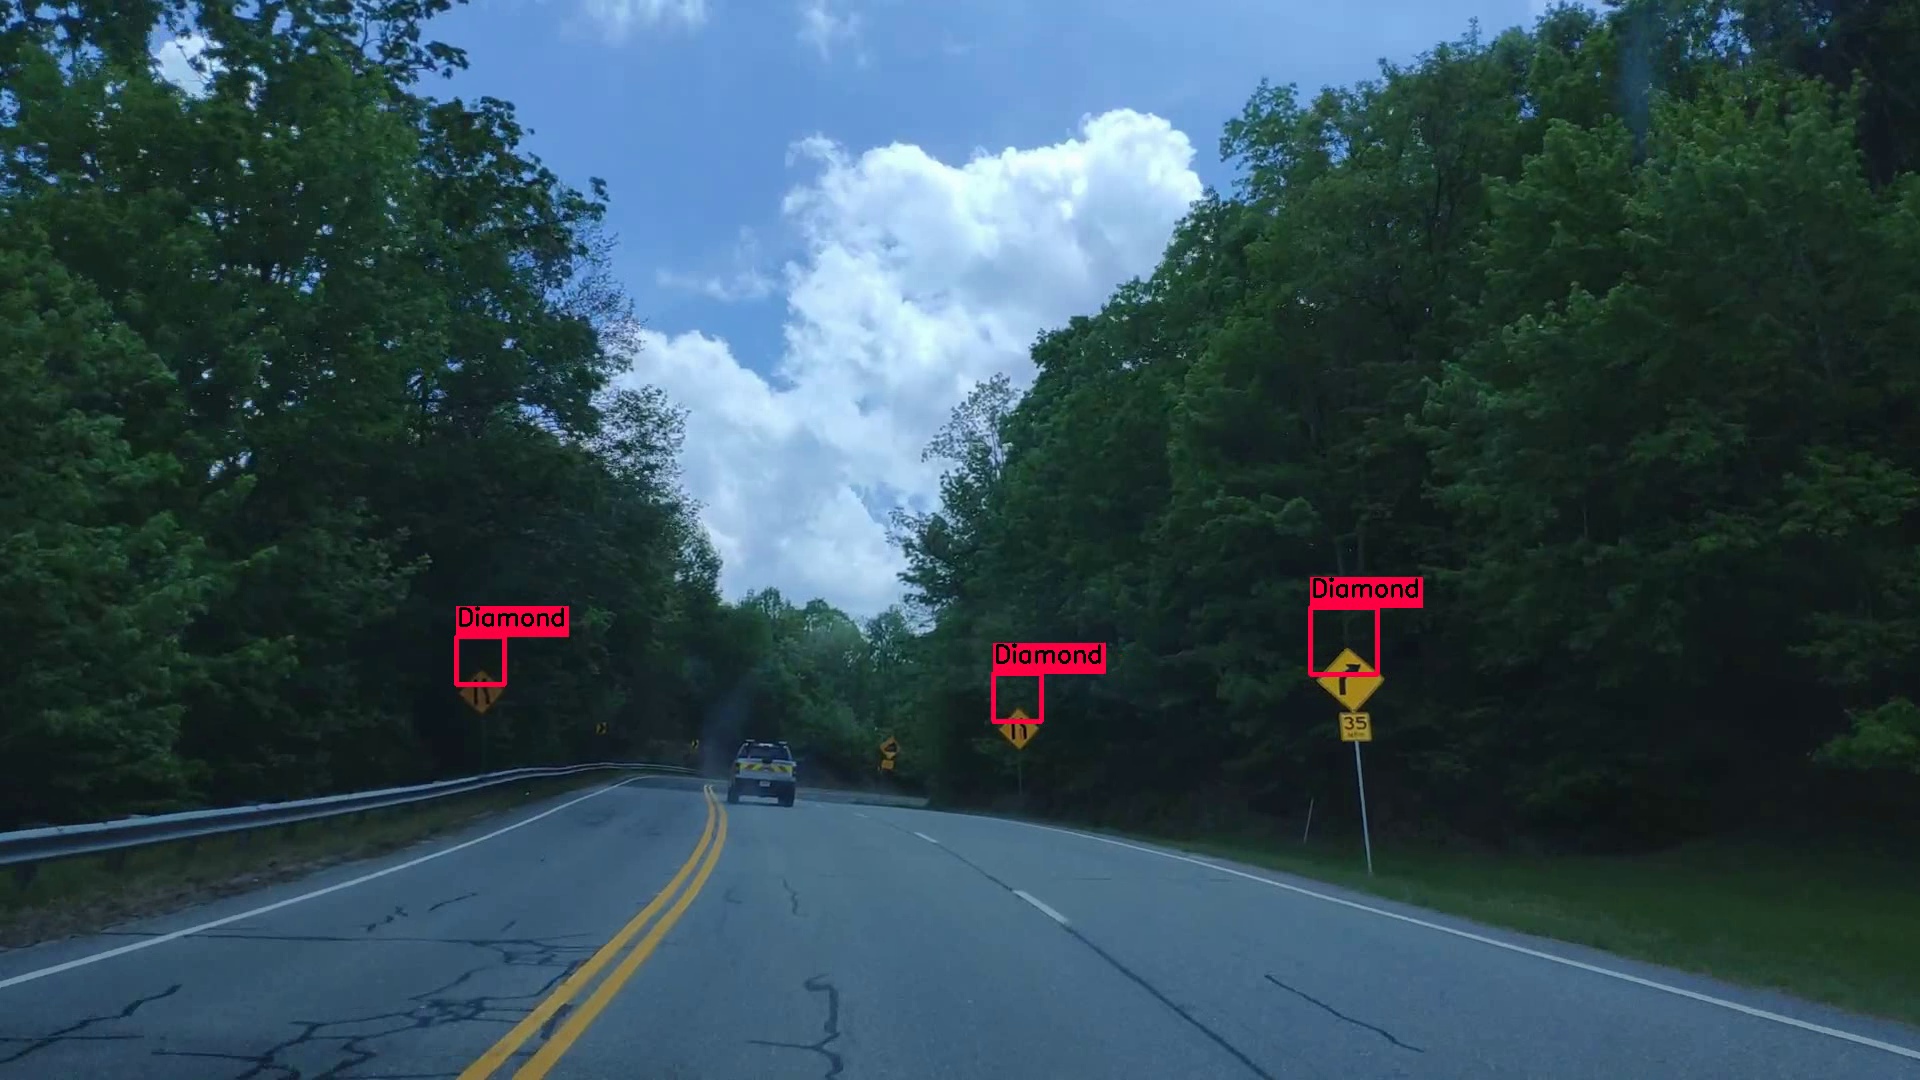
\includegraphics[width=0.99\linewidth]{figures/examples/sr2/TP/TP_05.png}
      \caption{Multiple signs in different conditions}
      \label{fig:multipleTP}
    \end{subfigure}
    \begin{subfigure}[t]{.49\linewidth}
      \centering
      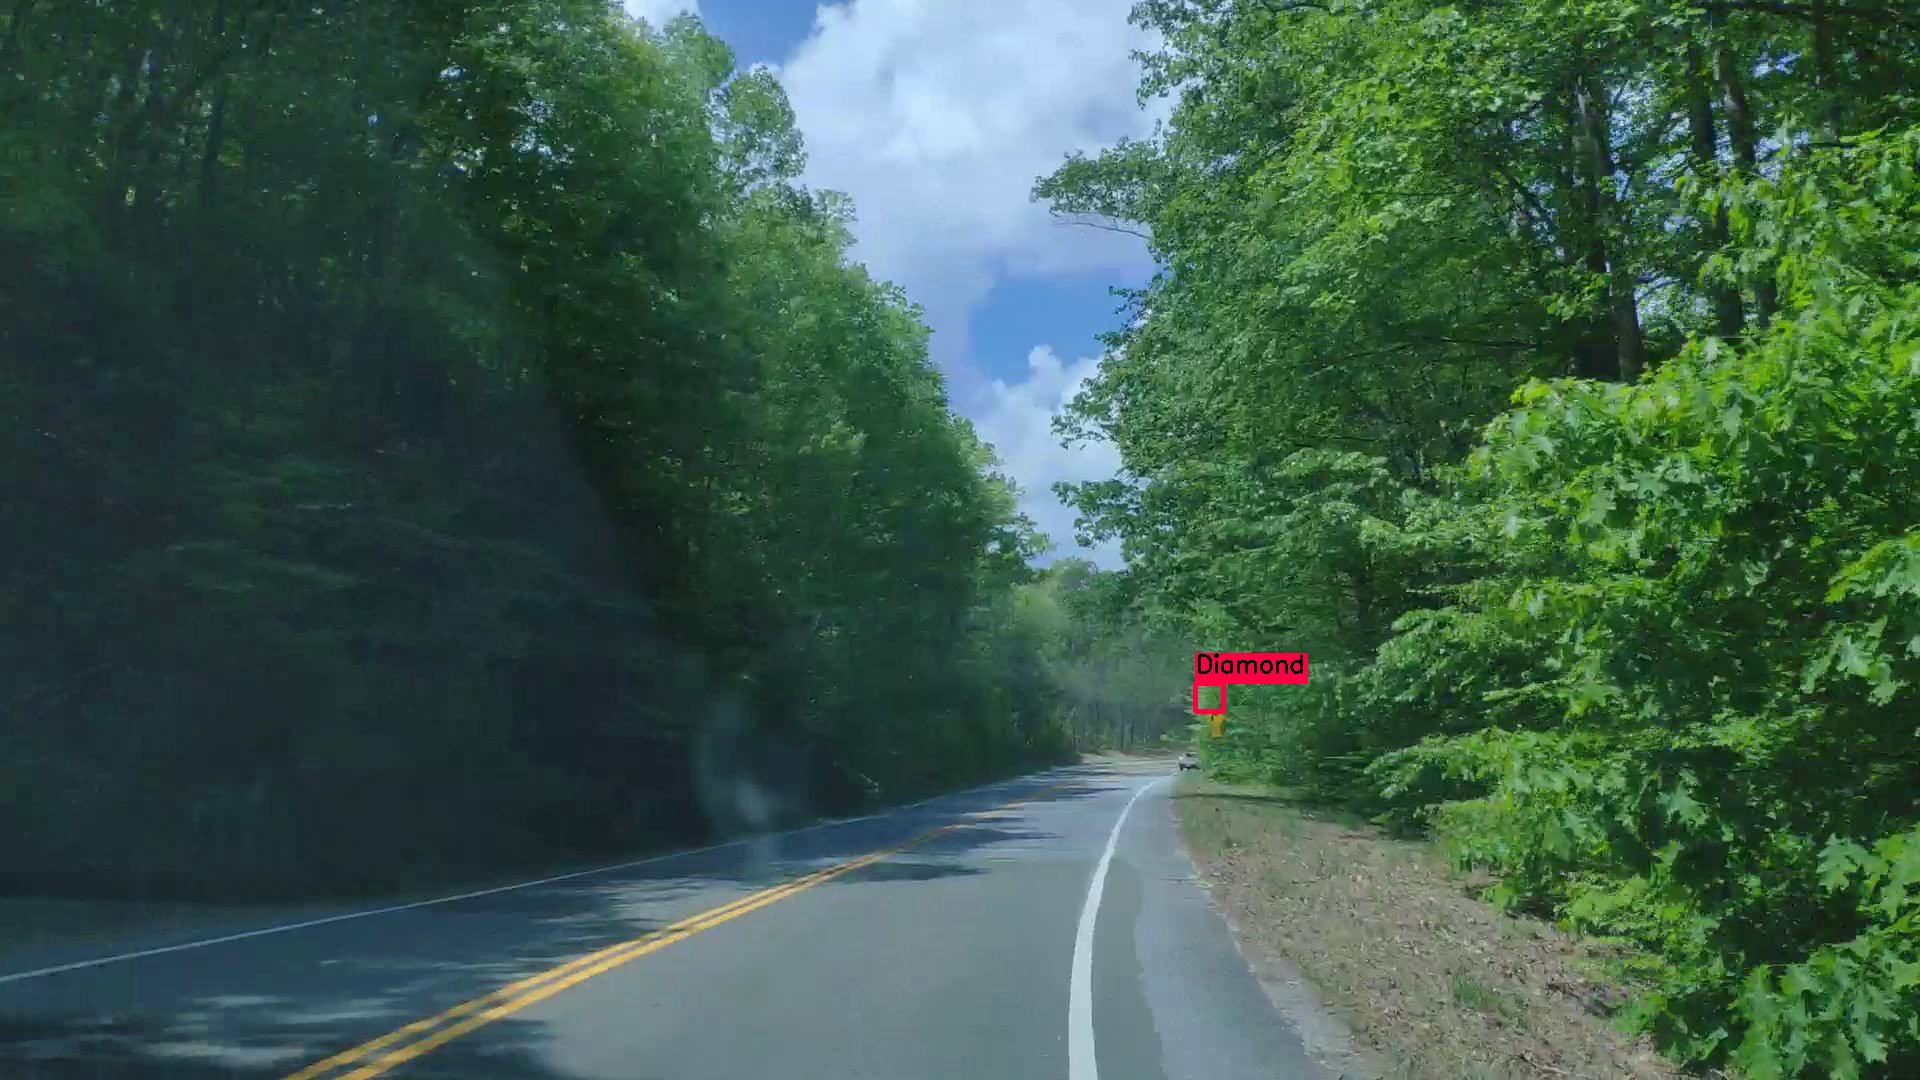
\includegraphics[width=0.99\linewidth]{figures/examples/sr2/TP/TP_08.png}
      \caption{Small sign}
      \label{fig:smallTP}
    \end{subfigure}
    \begin{subfigure}[t]{.49\linewidth}
      \centering
      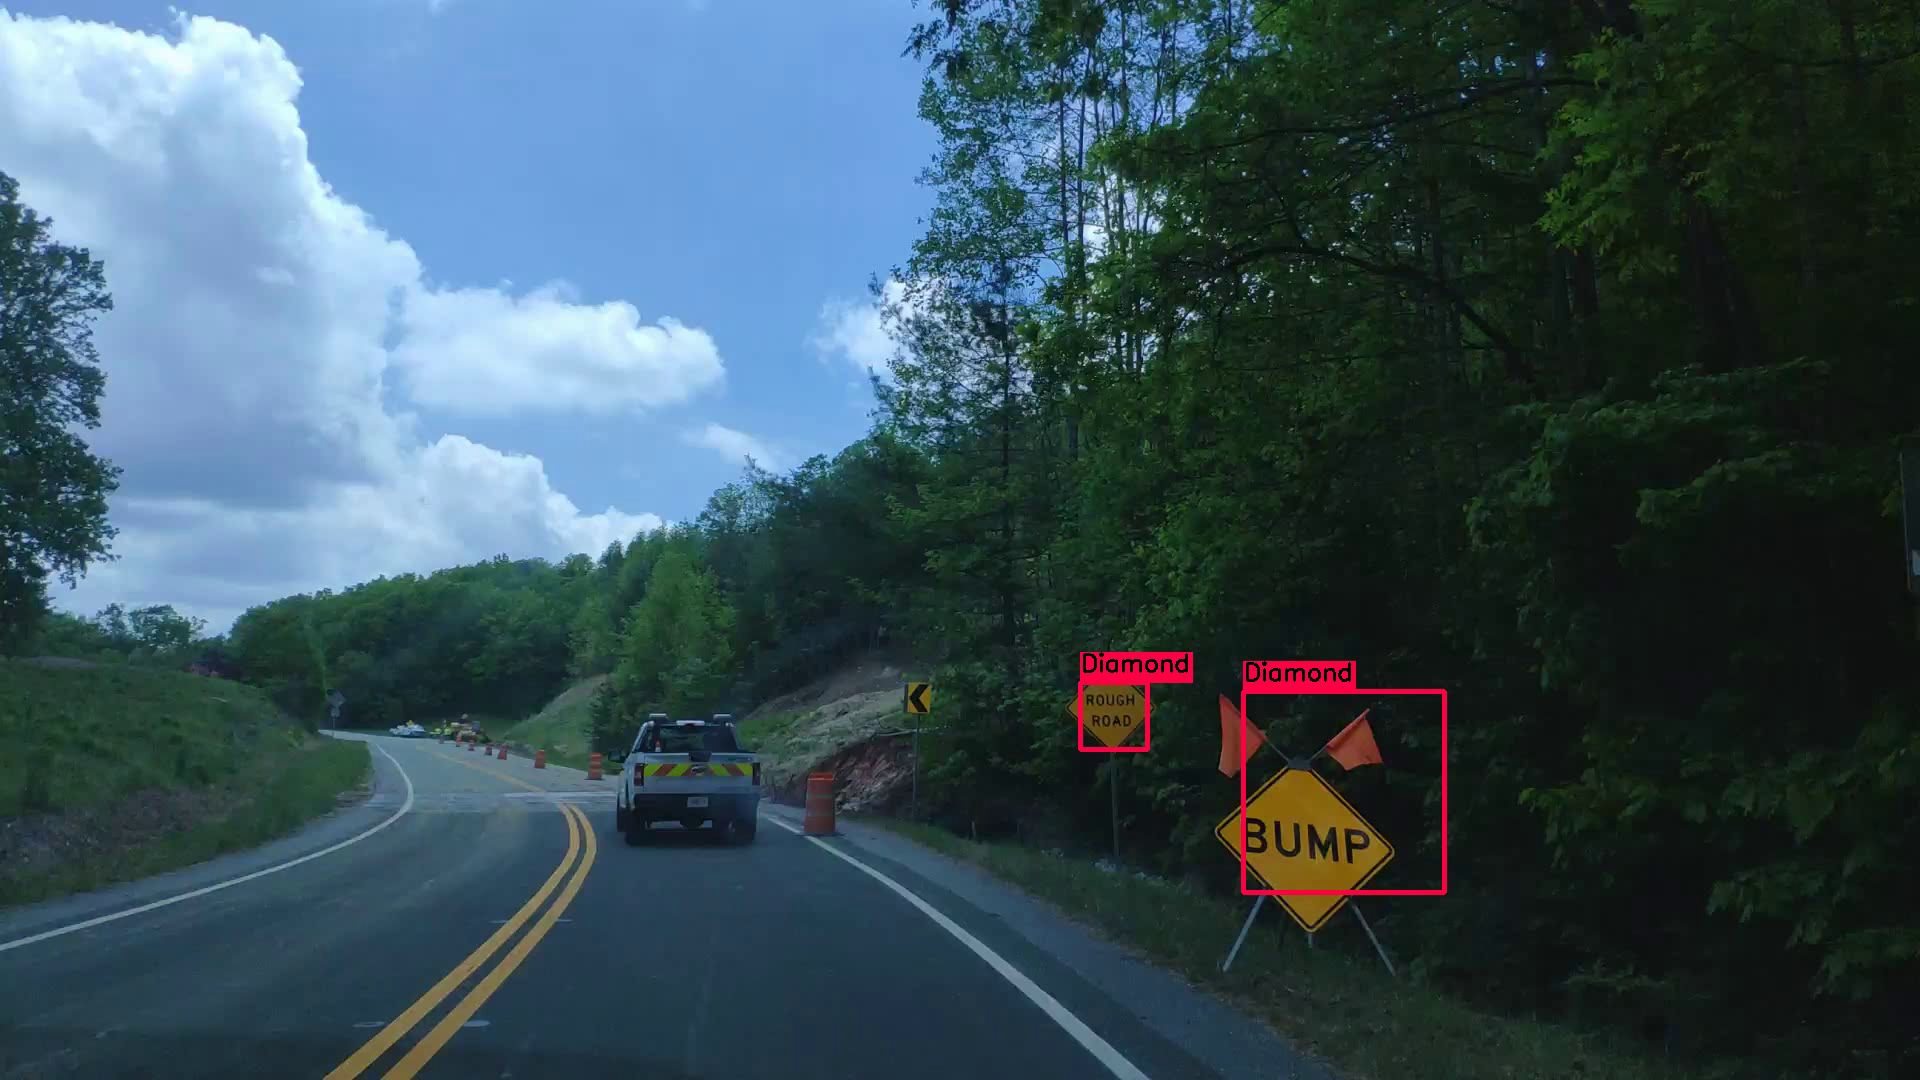
\includegraphics[width=0.99\linewidth]{figures/examples/sr2/TP/TP_02.png}
      \caption{Temporary sign of different size}
      \label{fig:bigtempTP}
    \end{subfigure}
    \begin{subfigure}[t]{.49\linewidth}
      \centering
      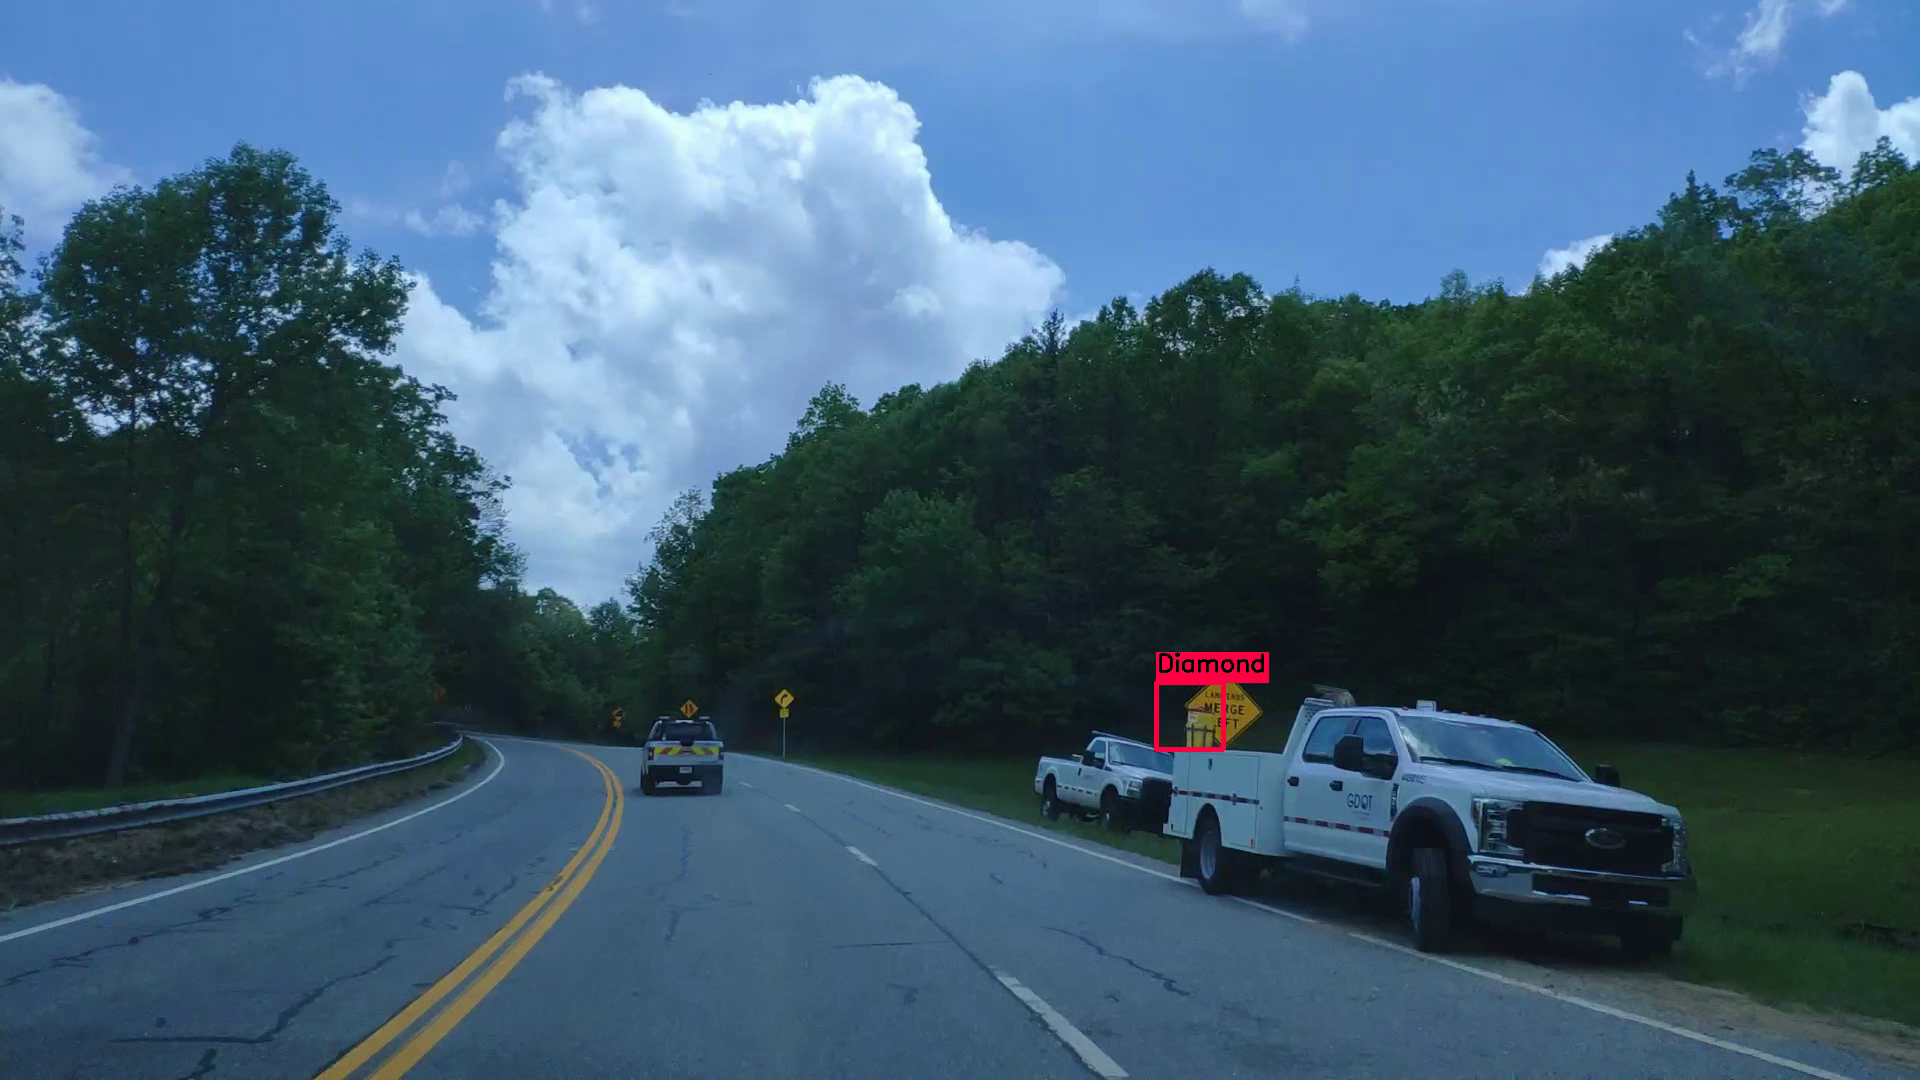
\includegraphics[width=0.99\linewidth]{figures/examples/sr2/TP/TP_04.png}
      \caption{Obstructed Sign}
      \label{fig:obstTP}
    \end{subfigure}
    \caption{Example of True positive cases collected on State Road 2.}
    \label{fig:TPcases}
  \end{center}
\end{figure}

\paragraph{}
Given the simplicity and the input size of our model, during our review, we were pleased to note different cases of True Positive (TP). One of them are the temporary warning signs displayed on Figure \ref{fig:temporaryTP} and \ref{fig:bigtempTP}, these signs are not part of our training data and are slightly different from the sign usually on the road, we were so pleased to see the model generalize on that point. Given the size of the input and the smallest possible anchors, $3\times3$, we were not expecting much detection at this size, but our experiment proved us wrong with lot of small sign being accurately detected, as you can see on Figure \ref{fig:smallTP}. Another difficult case that is not well represented on our dataset is the obstructed case. We did not do anything to help the network understand that sign could be hidden, but the model still manage to detect them properly, as you can see on Figure \ref{fig:obstTP} or also on Figure \ref{fig:farobstTP}, where the signs are barely visible on the full resolution image.

\subsection{West Westley}
\subsubsection{Presentation}
\paragraph{}
West Westley is another usually test site for our team, located in the residential area near Atlanta, it has been chosen because of the easy access it provides and its small curvy road with lot of vegetation around, making the signs sometimes difficult to detect. If this road is a usual test bed for our team, our training data does not include any of these roads.

\begin{figure}
    \centering
    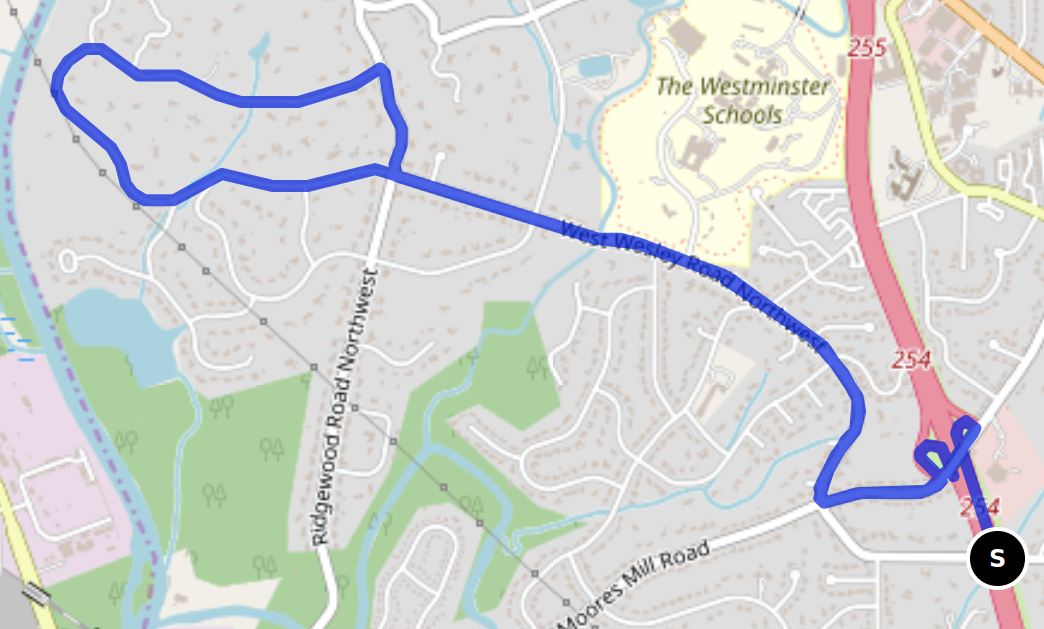
\includegraphics[width=0.8\linewidth]{figures/westwestleymap.png}
    \caption{Map representation of the West Westley test road.}
    \label{fig:wwmap}
\end{figure}{}

This test section is a 9km (5.6 Miles) long road in a residential area. As you can see on Figure \ref{fig:wwmap}, this road goes into lot of curves in high population area, but out of main large roads. The video collected is composed of $22,198$ frames, on witch we counted $34$ diamond warning signs. After reviewing the 12 minutes long video we got $10$ false positive cases (FP), $3$ false negative (FN) and $31$ true positive (TP). These numbers are also given on table \ref{tab:ww_numbers}, were you can see that our final precision is over two third, meaning that over two third of the object detected are actual diamond warning sign, this number goes even higher if you think in term of frames, as FP detection are generally limited to less than three frames. In term of recall, we get over the $90\%$ threshold, meaning that most of the signs are detected, and as we will see in the following, the missed signs represented difficult cases.

\begin{table}[]
    \centering
    \caption{Quantitative results for the test on West Westley. The numbers are given based on individual signs or object detected not on frame with detection.}
    \begin{tabular}{|c|c|c|c|c|c|c|}
        \hline
        Frame count & Sign count & TP & FP & FN & Precision & Recall \\ \hline
        $22,198$ & $34$ & $31$ & $10$ & $3$ & $76\%$ & $91\%$ \\ \hline
    \end{tabular}
    \label{tab:ww_numbers}
\end{table}{}

In the following we are going to give more detail about what is the reality behind these numbers, illustrating how our model behave in real application in this kind of context.

\subsubsection{False Positive cases}
\begin{figure}
  \begin{center}
    \begin{subfigure}[t]{.49\linewidth}
      \centering
      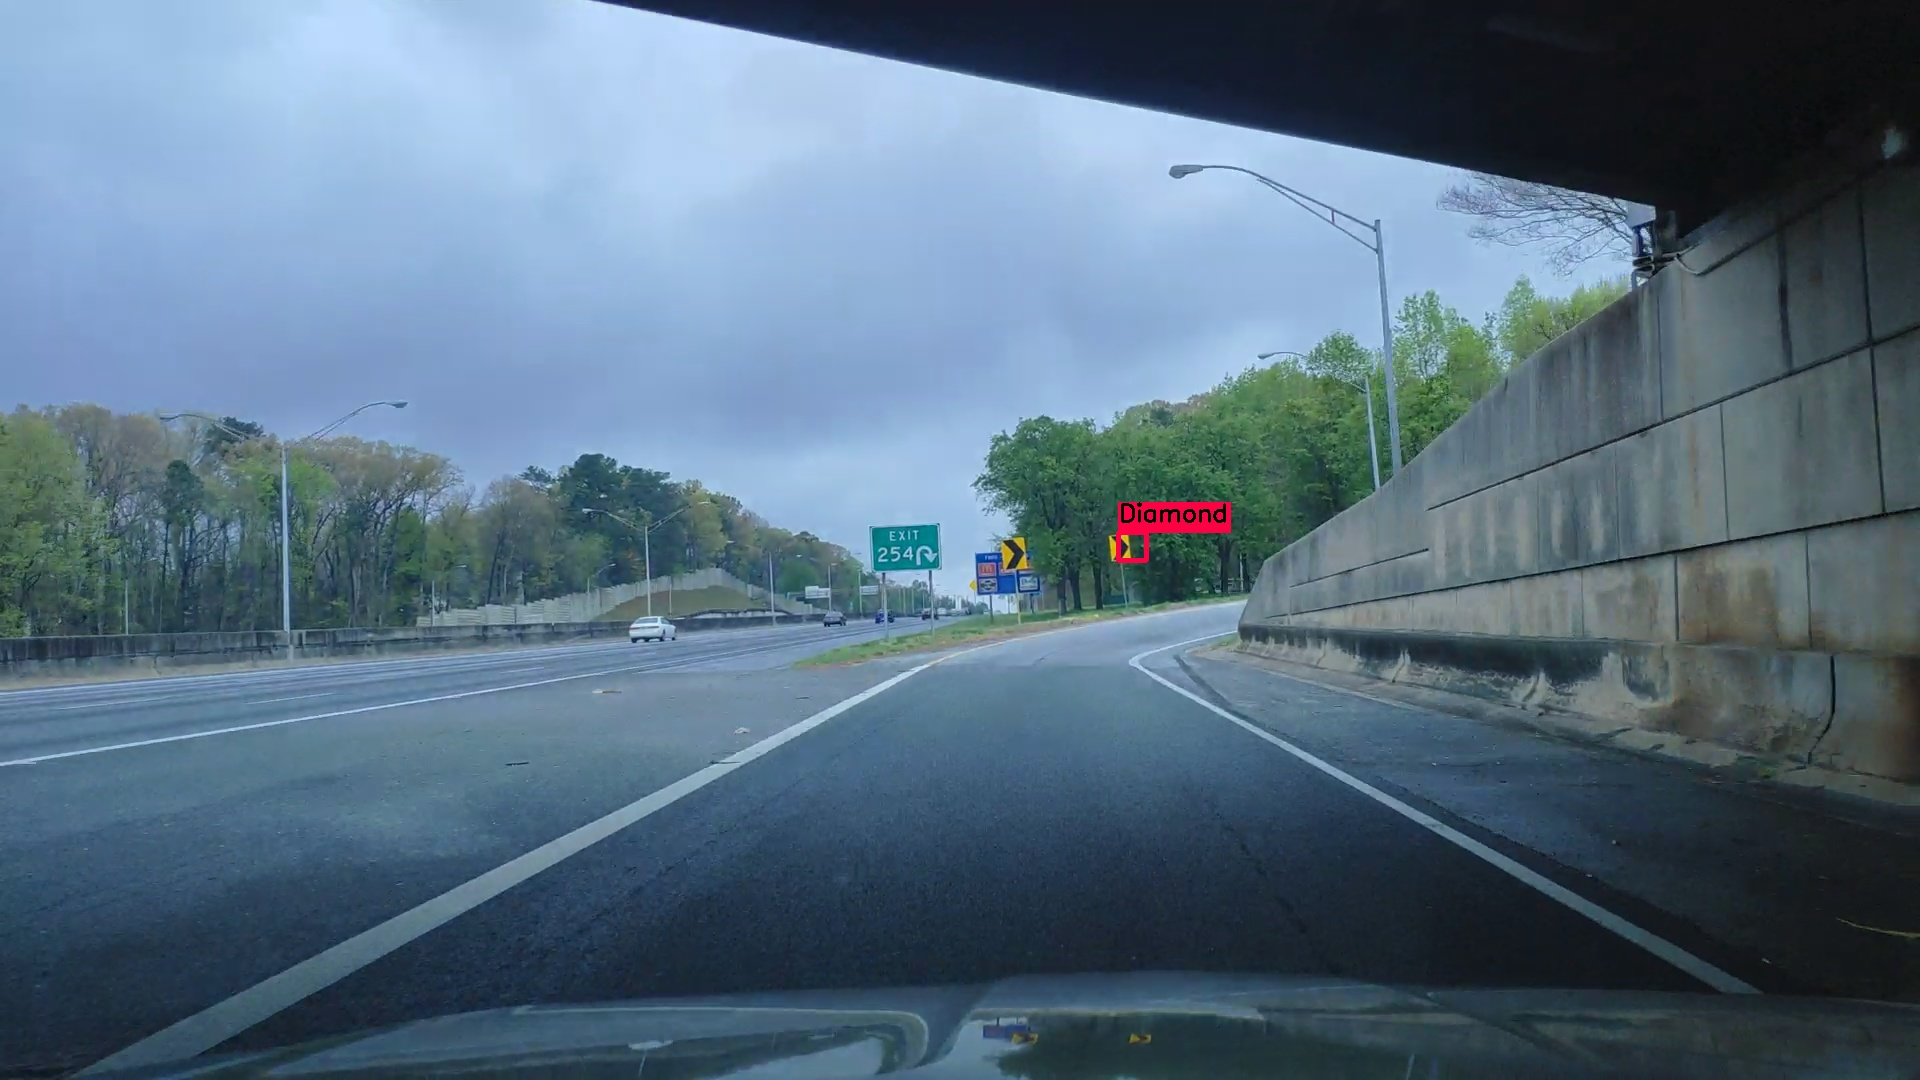
\includegraphics[width=0.99\linewidth]{figures/examples/westwestley/FP/FP01.jpg}
      \caption{Chevron sign}
      \label{fig:wwChevronFP}
    \end{subfigure}
    \begin{subfigure}[t]{.49\linewidth}
      \centering
      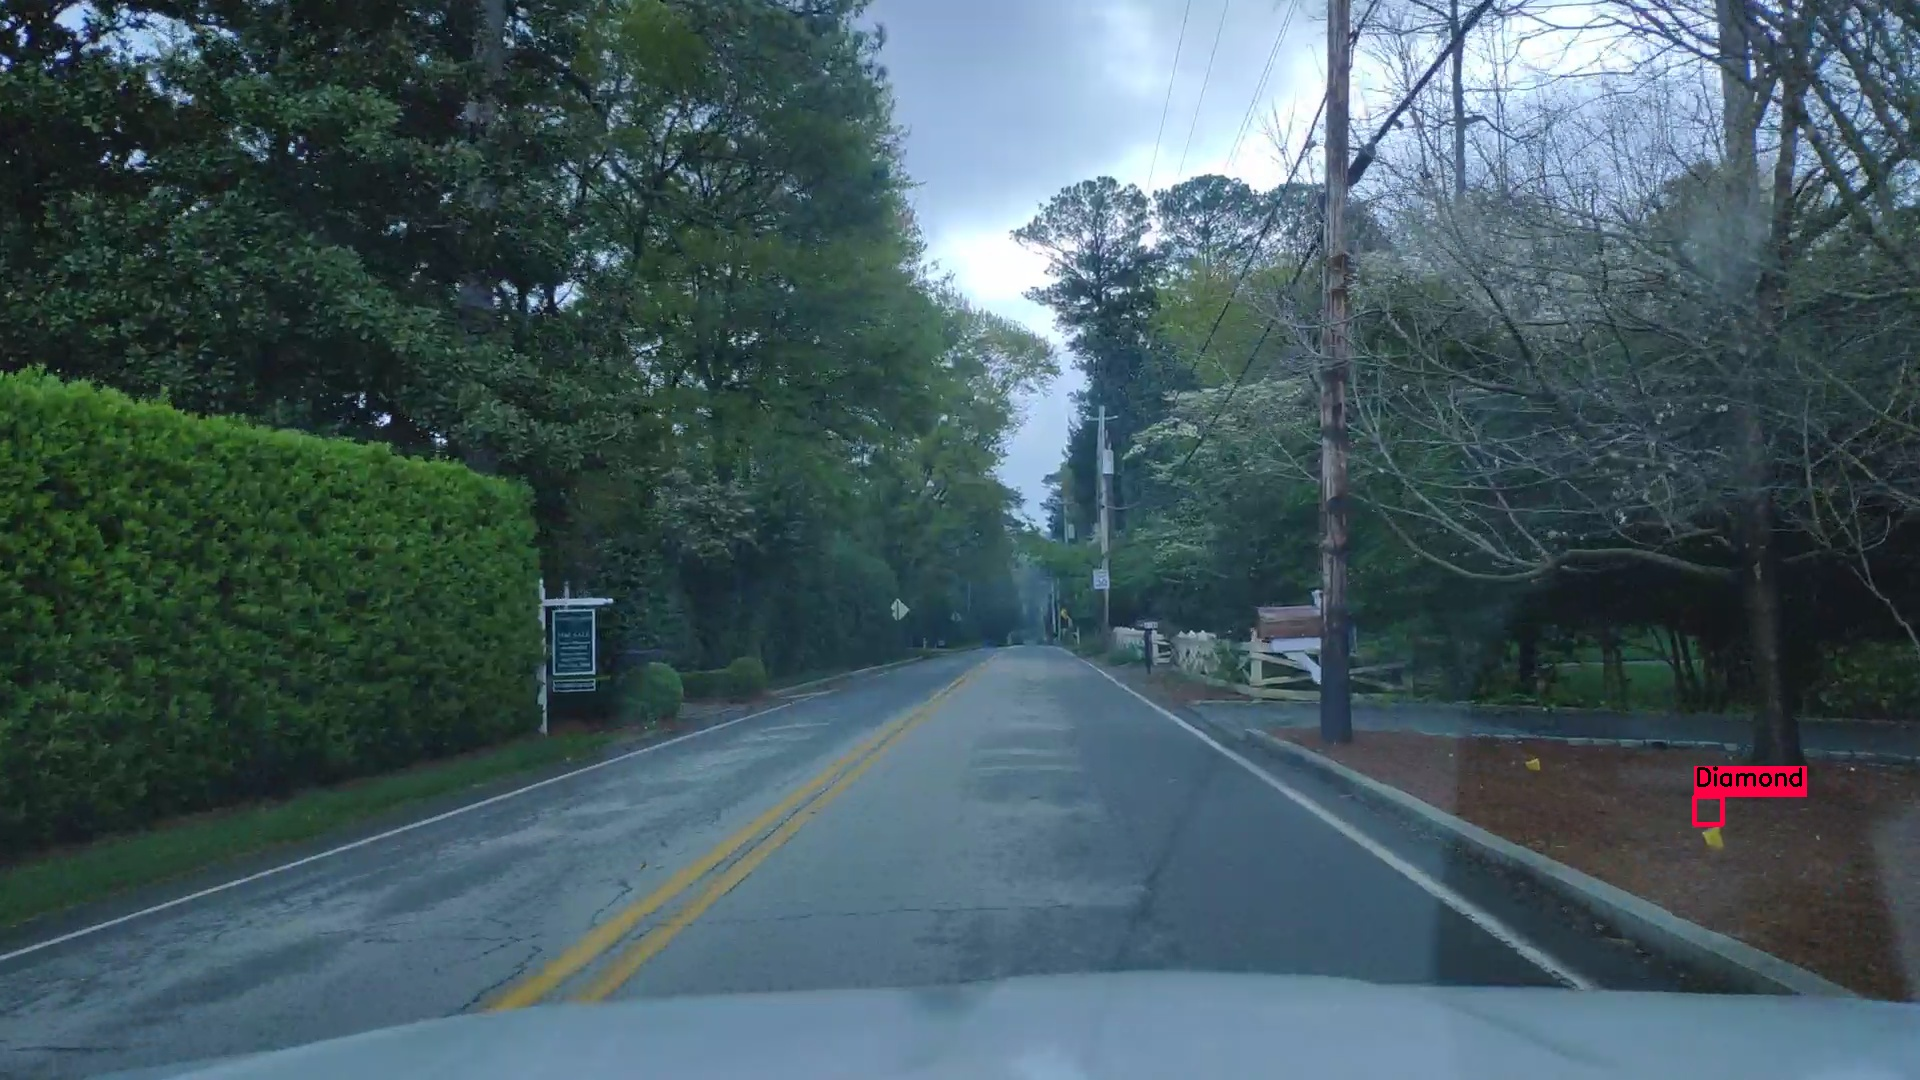
\includegraphics[width=0.99\linewidth]{figures/examples/westwestley/FP/FP02.jpg}
      \caption{Small yellow flag}
      \label{fig:wwFlag1FP}
    \end{subfigure}
    \begin{subfigure}[t]{.49\linewidth}
      \centering
      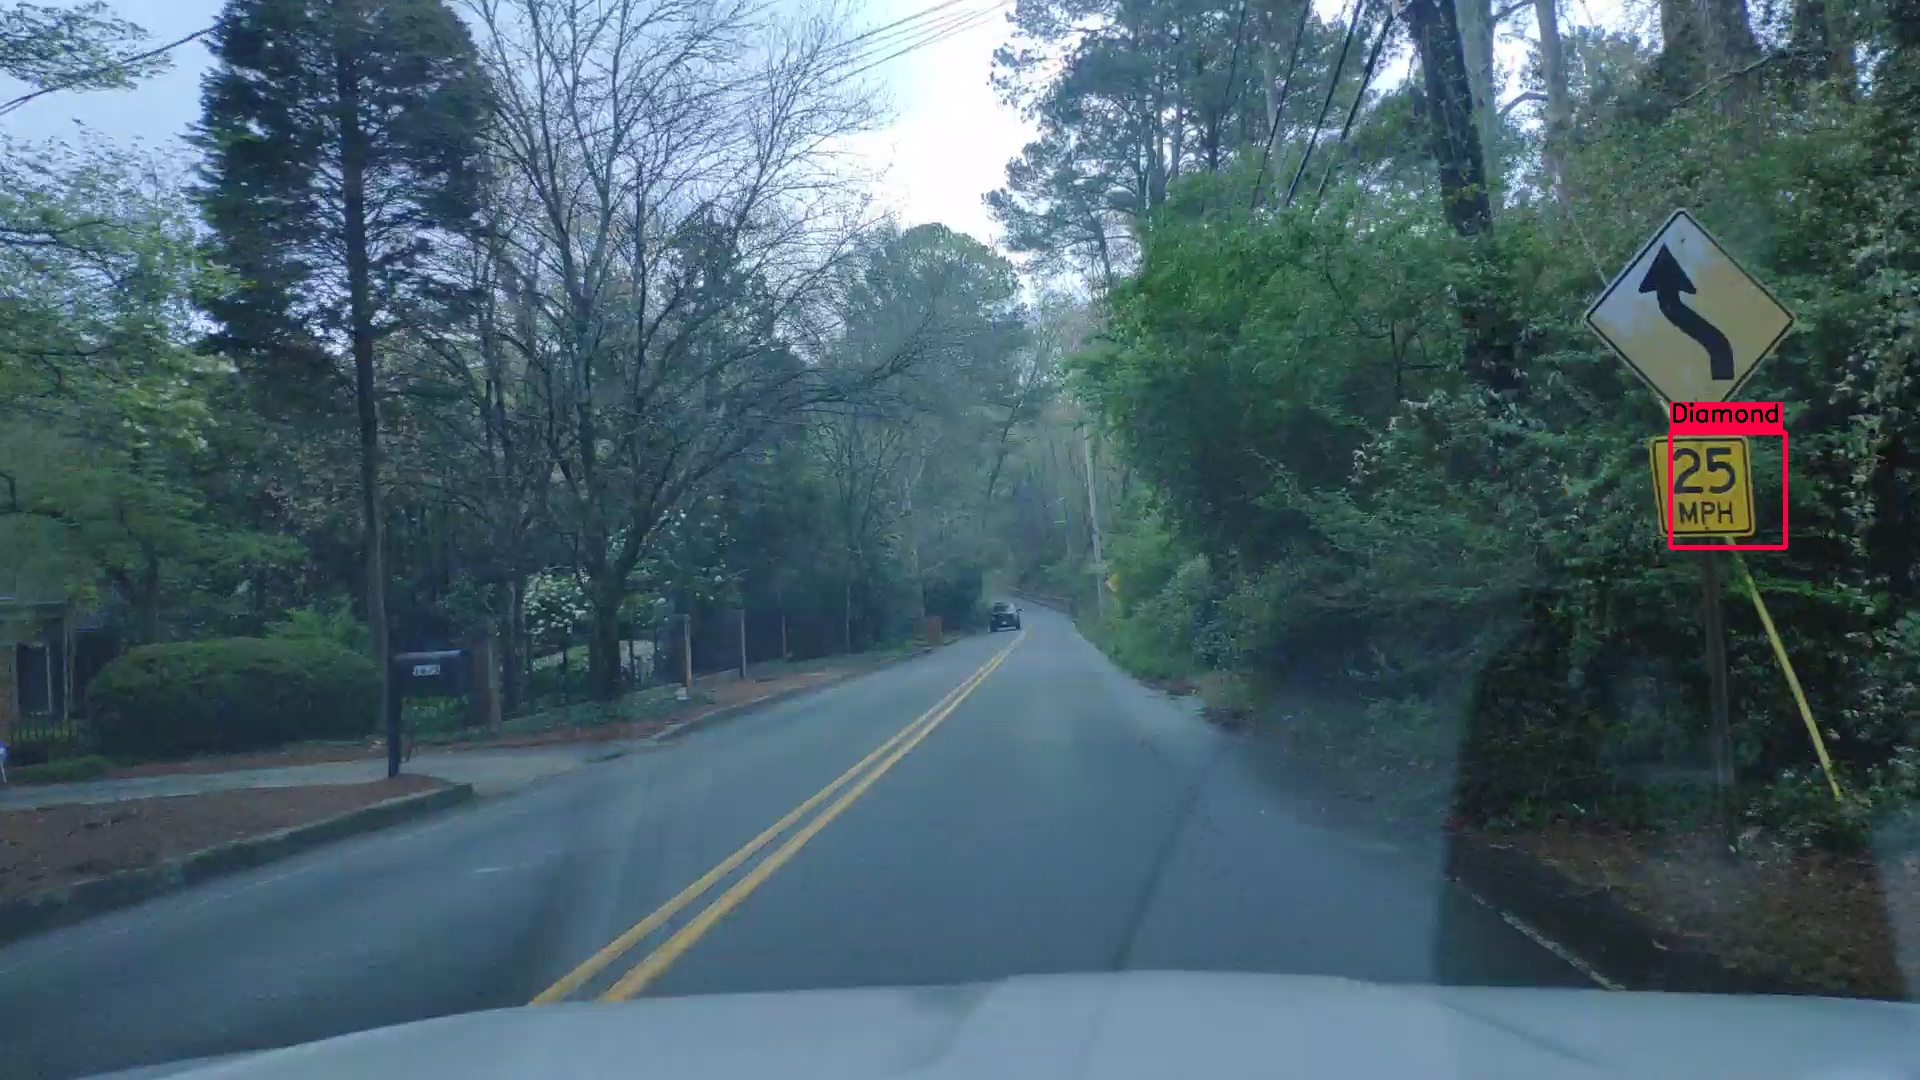
\includegraphics[width=0.99\linewidth]{figures/examples/westwestley/FN/FN01.jpg}
      \caption{Speed limit}
      \label{fig:wwslFP}
    \end{subfigure}
    \begin{subfigure}[t]{.49\linewidth}
      \centering
      \includegraphics[width=0.99\linewidth]{figures/examples/westwestley/FP/FP05.jpg}
      \caption{School Sign (MUTCD: S1-1)}
      \label{fig:wwSchoolFP}
    \end{subfigure}
    \begin{subfigure}[t]{.49\linewidth}
      \centering
      \includegraphics[width=0.99\linewidth]{figures/examples/westwestley/FP/FP06.jpg}
      \caption{Back of traffic light}
      \label{fig:wwTraffficLight1FP}
    \end{subfigure}
    \begin{subfigure}[t]{.49\linewidth}
      \centering
      \includegraphics[width=0.99\linewidth]{figures/examples/westwestley/FP/FP07.jpg}
      \caption{Chevron sign}
      \label{fig:wwChevron2FP}
    \end{subfigure}
    \begin{subfigure}[t]{.49\linewidth}
      \centering
      \includegraphics[width=0.99\linewidth]{figures/examples/westwestley/FP/FP08.png}
      \caption{Temporary sign}
      \label{fig:wwTemporaryTP}
    \end{subfigure}
    \begin{subfigure}[t]{.49\linewidth}
      \centering
      \includegraphics[width=0.99\linewidth]{figures/examples/westwestley/FP/FP09.png}
       \caption{Back of traffic light}
      \label{fig:wwTraffficLight2FP}
    \end{subfigure}
    \caption{Example of false positive cases collected on West Westley.}
    \label{fig:wwFPcases}
  \end{center}
\end{figure}

\paragraph{}
Of the $10$ FP detection on this test, $5$ are actual traffic signs and $1$ is a temporary traffic sign. The most common case of sign being detected is, as in Section \ref{sec:sr2} about state road 2, chevron signs. Example of such detection are given on Figure \ref{fig:wwChevronFP} and \ref{fig:wwChevron2FP}. Another sign that was mistaken as a diamond warning sign is the school warning sign, as displayed on Figure \ref{fig:wwSchoolFP}. This sign is special as it has an irregular pentagon shape with the top half looking exactly as a diamond sign. We also get the interesting case of a warning speed limit being detected, while the actual sign above it is not, this case is displayed on Figure \ref{fig:wwslFP}. The last case of sign that was miss detected is the temporary board displayed on Figure \ref{fig:wwTemporaryTP}.

The remaining false positive consist of the yellow back of traffic light as illustrated by Figure \ref{fig:wwTraffficLight1FP} and \ref{fig:wwTraffficLight2FP} and of small yellow construction flag on the side of the road, which you can see on Figure \ref{fig:wwFlag1FP}.

All this exact false positive cases were also encountered in other models trained over the same training data, this model, namely Yolov3-spp, is much more complex than our currant model, the fact that it still produce the same mistake raise large question about the coverage of the dataset we use. We were even surprised that our model detect them less frequently than the Yolov3-spp model, this is probably due to the smaller complexity of our model forcing it to generalize more. All this False Positive cases are only detected on less than five frames showing that adding a few more example during training could improve the results a lot.

\subsubsection{False Negative cases}
\paragraph{}
This test section revealed three different case of false positive. The first one, displayed on Figure \ref{fig:wwWhiteFN}, was already encountered in Section \ref{sec:sr2}, it consists of a whitened and faded sign with not very bright yellow color. The case of Figure \ref{fig:wwFaddedFN} is even more difficult, the sign is covered by a green algae and under the shadow of a pine tree making it particularly difficult to detect. Finally, the last case of False Negative detection happen on the ramp to exit the high way, it consists of a sign on the edge of the video, often obstructed by the sign in front of it. In addition, this sign that you can see on Figure \ref{fig:wwobsFN}, is whiter than usual, a case that our model as trouble to detect.
\begin{figure}
  \begin{center}
    \begin{subfigure}[t]{.49\linewidth}
      \centering
      \includegraphics[width=0.99\linewidth]{figures/examples/westwestley/FN/FN01.jpg}
      \caption{Whitened sign}
      \label{fig:wwWhiteFN}
    \end{subfigure}
    \begin{subfigure}[t]{.49\linewidth}
      \centering
      \includegraphics[width=0.99\linewidth]{figures/examples/westwestley/FN/FN02.jpg}
      \caption{Dirty, faded sign in the shadow}
      \label{fig:wwFaddedFN}
    \end{subfigure}
    \begin{subfigure}[t]{.49\linewidth}
      \centering
      \includegraphics[width=0.99\linewidth]{figures/examples/westwestley/FN/FN03.png}
     \caption{Small often obstructed sign}
      \label{fig:wwobsFN}
    \end{subfigure}
    \caption{Example of false negative cases collected on West Westley.}
    \label{fig:wwFNcases}
  \end{center}
\end{figure}


\subsubsection{Interesting True Positive cases}
\paragraph{}
Considering the simplicity of our model and the input resolution, we were pleased to see that we were able to manage all the cases where the signs were obstructed by trees on this road. Figure \ref{fig:wwTPcases} show some example of such successful detection in non-trivial cases.

\begin{figure}
  \begin{center}
    \begin{subfigure}[t]{.49\linewidth}
      \centering
      \includegraphics[width=0.99\linewidth]{figures/examples/westwestley/TP/TP04.jpg}
      \caption{Obstructed sign}
      \label{fig:wwObs1TP}
    \end{subfigure}
    \begin{subfigure}[t]{.49\linewidth}
      \centering
      \includegraphics[width=0.99\linewidth]{figures/examples/westwestley/TP/TP02.jpg}
      \caption{Obstructed sign}
      \label{fig:wwObs2TP}
    \end{subfigure}
    \begin{subfigure}[t]{.49\linewidth}
      \centering
      \includegraphics[width=0.99\linewidth]{figures/examples/westwestley/TP/TP05.png}
      \caption{Obstructed sign}
      \label{fig:wwObs3TP}
    \end{subfigure}
    \caption{Example of true positive cases collected on West Westley.}
    \label{fig:wwTPcases}
  \end{center}
\end{figure}

\subsection{Conclusion}
\paragraph{}
In this section we demonstrated the generalization of our results on the validation data to real use cases. Showing that, if the accuracy of our model does not reach state-of-the-art object detection levels, it does achieve very good results, that can be used on real live while speeding up the detection process by a one hundred factor allowing to be run directly on a smartphone.

\section{About localization}
\paragraph{}
You probably noticed on all the images examples given previously, that most of the time the detection box is off the sign and is not perfectly at the right size. There is even cases like on Figure \ref{fig:multipleTP} where the box is completely outside the sign. To interpret this results, it is important to remember the assumption from Chapter \ref{chapter:technicalApproach} Section \ref{Assumptions}. Our model is not trying to draw a perfect box around an object, but is instead trying to give the approximate position and approximate size of the object to detect. 

In most of the application this approximated position and size are enough to get what you need, especially in a traffic sign detection context where getting pixel accurate box around the sign does not add lot of value. Even if this accuracy is not enough for a given task, the computation speed to get this results is so fast that you that you can use a post processing that will refine the box locally and still be faster than other larger models because you will skip most of the useless frames.

\section{Conclusion}
\paragraph{}
In this chapter we used the tools defined in Chapter \ref{chapter:technicalApproach} to build an efficient architecture, exploring its behavior over our dataset. We trained it over our artificial dataset and showed the improvement it brings to the final results. We finally studied the results of our model in term of computation efficiency, comparing it to well known architecture, and concluded by testing the resulting model on real live application, to exhibit the strange and weakness of our approach, showing that this approach successfully solve our problem and is ready for real life usage. However, improvement can still be made and lot of open research question are still unsolved, calling for additional research on that field.



